\documentclass[
  utf8,%     More capable input encoding than latin-1.
  % parskip,%  For vertical whitespace between paragraphs.  This comes down to more than just using parskip.sty, so it's better to use this class option.
  % S5MP % If you intend to really use margin paragraphs (not recommended!).
%  crop,%     Produce output with crop marks and paper size A4.  Liu-Tryck should like this.  Automatically adds information, including the physical page number, at the top of each page.
       %     Add option 'noInfo' to suppress the info at the top of each page when using option 'crop'.
  % Font options: 'kp' (default), 'times', 'lm'.  The KpFonts (loaded using 'kp'), is the most complete font among the provided options.  Among other, it supports slanted small caps.  See rtthesis.cls for more details regarding the font options.
  largesmallcaps,intlimits,widermath,% Good options to KpFonts.
  sharecounter,nobreak,definition=marks,%  See comments in the results chapter of this document for more information on these options!
  numbers, % If you want to cite references by numbers, use this option.
  noparts% Use option 'noparts' if you do not make use of part divisions.
]{rtthesis}

\usepackage{mythesis}
\usepackage{tikz}
\usepackage{algorithm}
\usepackage{algpseudocode}
\usepackage{todonotes}
\usepackage{subfig}
\usetikzlibrary{calc}
\usetikzlibrary{plotmarks}
\usetikzlibrary{shapes}
\usetikzlibrary{arrows}
\usetikzlibrary{positioning}

\renewcommand{\vec}[1]{
    \boldsymbol{#1}
}

\newcommand{\uvec}[1]{
    \boldsymbol{\hat{#1}}
}

\newcommand{\Arg}[1]{
    \mathrm{Arg}~#1
}

\DeclareMathOperator*{\argmax}{arg\,max}
\DeclareMathOperator*{\argmin}{arg\,min}

\newcommand{\Drone}[3]{
  \draw[
    fill=gray,
    rounded corners=1mm,
    rotate around={#3:(#1,#2)}
  ] (#1,#2) --++ (-.5,.35) --++ (0.25,-.35) --++ (-0.25,-.35) -- (#1,#2);
}

\tikzstyle{point} = [
  circle,
  minimum width=3.5pt,
  inner sep=0,
  fill=black
]

\tikzstyle{my_v} = [
  ->,
  line width = 1.2pt
]

\tikzstyle{block} = [rectangle, draw, fill=blue!20, 
text width=5em, text centered, rounded corners, minimum height=4em]
\tikzstyle{line} = [draw, -latex']

\begin{document}
\selectlanguage{english}

\frontmatter
\maketitle

\begin{abstract}[english]
  Fixed-wing \acp{uav} are today used in many different areas, from agriculture to search and 
rescue operations. Through various research efforts, they are becoming more and more autonomous. However, the procedure of landing a fixed-wing \ac{uav} 
remains a challenging task, which requires manual input from an experienced pilot. 

This work proposes a novel method which autonomously performs such landings. The main focus is on 
small and light-weight \acp{uav}, for which the wind acts as a major disturbance and has to be taken into account. 
Robustness to other disturbances, such as variations in environmental factors or measurement errors, has also been prioritized during the development 
of this method.

The main contribution of this work consists of a framework in which der\-iva\-tive-free optimization is used to 
calculate a set of waypoints, which are feasible to use in different wind speeds and directions, for a selected \ac{uav} model. 
These waypoints are then combined online using motion planning techniques, to create a trajectory which safely brings the \ac{uav} to a 
position where the landing descent can be initiated. To ensure a safe descent in a predefined area, another non-linear optimization problem is 
formulated and solved. 

Finally, the proposed method is implemented on a real \ac{uav} platform. A number of simulations in different wind conditions are performed, and data from 
a real flight experiment is presented. The results indicate that the method successfully calculates feasible landing sequences in different scenarios, and 
that it is applicable in a real-world landing.


\end{abstract}

%\begin{acknowledgments}
I would like to begin by thanking my co-founder of Airpelago and supervisor Fredrik Falkman. 
Without your hard work and visionary mindset the past years, neither Airpelago nor this thesis project would exist.

At Linköping University, I would like to thank my supervisors Jonatan Olofsson and Kristoffer Bergman. You have been a 
constant source of valuable feedback and suggestions. I would also like to thank my examiner Daniel Axehill for always being open to 
new ideas and helping me setting a reasonable scope for this thesis.

Last but definitely not least, I would like to thank my family and friends. Without your constant support,
this thesis would not have been possible. A special thanks to all the people that I've shared the last years in Linköping with. 
You have made my university studies a real highlight of my life so far!

  \addvspace{1em}
  \begin{flushright}
    \textit{%
      Linköping, April 2020\\
      Tobias Fridén%
    }
  \end{flushright}
\end{acknowledgments}


\tableofcontents
%\begin{notation}% Passing the option "old" to the notation environment will redefine the notationtabular environment so that it produces an old style LaTeX tabular instead of a booktabs.sty style tabular.
  \centering

  \begin{notationtabular}{Notation}{Symbol}{Meaning}
    $\vel$ & Velocity relative to the earth\\
    $\airvec$ & Velocity relative to the air\\
    $\windvec$ & Wind velocity \\
    $V$ & Speed relative to the earth \\
    $\airspd$ & Speed relative to the air\\
    $\windspd$ & Wind speed\\
    $\psi$ & Heading\\
    $\cog$ & Course over ground\\
    $\winddir$ & Wind direction\\
    $\states$ & Set of possible states\\
    $\xobst$ & States with obstacles\\
    $\actions$ & Set of available control inputs\\
    $\vec{p}_a$ & Landing approach point\\
    $\vec{p}_l$ & Landing touchdown point\\
    $\landing$ & Designated landing area\\

  \end{notationtabular}

  % \begin{notationtabular}{Förkortningar}{Förkortning}{Betydelse}
  %   \abbrARMA\index{ARMA@\abbrARMA!abbreviation} & Auto-regressive moving average \\
  %   \abbrPID\index{PID@\abbrPID!abbreviation} & Proportional, integral, differential (regulator) \\
  % \end{notationtabular}
\end{notation}


\mainmatter
%\chapter{Introduktion}\label{cha:intro}
Redan de gamla grekerna\index{greker} och rommarna trodde att\dots

\chapter{Introduction}

\section{Background}
Unmanned Aerial Vehicles (UAVs) have many different applications, both in commercial usecases such as construction and agriculture, but also in emergency response and personal use. 
UAVs can be divided into two subclasses, multirotors and fixed-wing UAVs. 
While both types of UAVs are becoming more and more autonomous through various research efforts, landing of fixed-wing UAVs remains a challenging task which 
requires manual input from an experienced pilot. For small and light-weight UAVs the presence of wind also acts as a major disturbance which has to be taken into account when planning 
the landing procedure.
\section{Scope}
\subsection{Problem formulation}
The aim of this thesis is to develop a framework for automatically generating feasible 
landing procedures for fixed-wing UAVs, under the presence of winds. The landing procedure should be able to take the UAV 
from an arbitrary initial position and land safely in a predefined landing area while fulfilling physical constraints of the system. 
This thesis aims to answer the following questions:
\begin{enumerate}
    \item How can sampling-based motion planning techniques be used to generate landing sequences for fixed-wing UAVs?
    \item How can safe landings be guaranteed when taking wind effects into account?
\end{enumerate}
\subsection{Aim and delimitations}
The components of a general autonomous system are illustrated in Figure \ref{fig:autonomous}. The work in this thesis 
is mainly focused on the motion planning component. However, the tracking controllers and parameters of the actual UAV have to be taken into account 
to ensure feasibility of the generated path. Furthermore, the main focus of this thesis is UAVs using the ArduPilot open source autopilot \cite{arduplane}.

\begin{figure}
    \begin{center}
        \begin{tikzpicture}[node distance = 3cm, auto]
            \node[block] (init){Behaviour layer};
            \node[block, dashed, below of=init] (user){User};
            \node[block, right of=init] (mp){Motion planning};
            \node[block, right of=mp] (ctrl){Tracking controllers};
            \node[block, right of=ctrl] (uav){UAV};

            \path[line] (user) -> node[midway, left]{Manual input} (init);
            \path[line] (init) -> node[midway, above, align=left, yshift=.9cm]{High-level \\ commands} (mp);
            \path[line] (mp) -> node[midway, above, align=left, yshift=.9cm]{Reference \\ trajectory} (ctrl);
            \path[line] (ctrl) -> node[midway, above, align=left, yshift=.9cm]{Actuator \\ outputs} (uav);
        \end{tikzpicture}
    \end{center}
    \caption{Components of a general autonomous system}
    \label{fig:autonomous}
\end{figure}

\section{Outline}
Chapter \ref{cha:fixed_wing_uav} introduces general concepts regarding fixed-wing UAVs and the kinematic models and controllers studied in this thesis.
Chapter \ref{cha:wind} defines the wind field and discusses methods to estimate wind.
Chapter \ref{cha:motion_planning} gives an overview of necessary motion planning theory. In Chapter \ref{cha:motion_planning_fw} the 
a motion planning framework for fixed-wing UAVs flying in wind is proposed.
Chapter \ref{cha:landing} describes the landing procedure of a fixed-wing UAV and how optimal landing parameters can be calculated. 
In Chapter \ref{cha:implementation} the implementation of the proposed framework on a real UAV platform is discussed. Chapter \ref{cha:results} presents experimental 
results which are discussed in chapter \ref{cha:discussion}.
\section{Related work}
\subsection{Motion planning}
Motion planning refers to the task of finding a feasible path between a initial state and a goal for a given system. Since this is an important component of autonomous systems it has received increasing research interest lately, with an array of different algorithms and methods available. 

\subsubsection{Sampling based motion planning}
Many motion planning techniques are based on discrete sampling of the continuous state - and action space. These methods are either based on 
random sampling, such as in Probabilistic Roadmaps \cite{prm} or Rapidly Exploring Random Trees \cite{rrt} while others such as Hybrid $A^*$ \cite{hybrid_astar} use 
deterministic sampling.

In \cite{2_phase_uav} the $A^*$ algorithm \cite{astar} is used to find kinematically feasible trajectories for fixed-wing UAVs with 
a maximum turn rate while avoiding obstacles. The feasibility of the resulting path is ensured by aligning the dimensions of the 
sampled grid with model parameters of the given UAV.

In \cite{wind_astar} the results in \cite{optimal_path_trochoidal} are used together with $A^*$ to generate time-optimal trajectories in the 
presence of wind, while also avoiding obstacles. They further define the region for where air-relative Dubins paths are not time-optimal 
based on the results in \cite{optimal_path_target} and use these results to modify the heuristic function.

A RRT-based motion planning framework for fixed-wing UAVs, with constraints on both arrival time and final direction is proposed in \cite{rrt_uav}.

\subsubsection{Optimal control approach}
The problem of finding time-optimal paths for fixed wing UAV:s in uniform winds formulated as an optimal control problem has been studied
by different authors. In these works the following kinematic model is used:
\begin{equation}
    \dot{x}=f(x, u)=
    \begin{bmatrix}
        V_a\cos\psi + W\cos\psi_w\\
        V_a\sin\psi + W\sin\psi_w\\
        u    
    \end{bmatrix} 
\end{equation}
where the input is the turn-rate $u$ which is constrained such as $|u|\leq\dot{\psi}_{max}$.
In \cite{optimal_path_target} the problem is reformulated as finding a path which 
intersects a virtual target moving from $x_g$ with the same speed as the wind but in the opposite direction. It is shown that in most cases,
the shortest path is a Dubin's path in the air-relative frame, but in some cases a non-Dubin's path is required to 
intercept the target. The optimal solution is found by defining the function
\begin{equation}
    G(d)=T_a(d) - T_{vt}(d)
\end{equation}
where $d$ is a given distance travelled by the virtual target, $T_a(d)$ is the minimal time at which the 
aircraft reaches the point where the target has travelled this distance and $T_{vt}$ is the required time for the virtual target. 
The optimal solution is found when $G(d)=0$ and can be solved for using numerical root-finding techniques.

The approach in \cite{optimal_path_trochoidal} is based on the observation from \cite{course_hdg_wind} that 
constant turn-rate paths in the air-relative frame correspond to \textit{trochoidal} paths in the inertial frame. 
They further show that there exists an analytical solution to compute some of the optimal-path candidates, but to find 
all possible optimal paths a trandescendal equation has to be solved on a two dimensional grid which is computationally expensive.

\subsection{Landing approaches}
The problem of autonomously landing fixed-wing UAVs in different settings has been studied by several authors. 
In many of these works, the problem is defined as landing the UAV on a runway. A survey of different landing techniques is given in \cite{survey_landing}.
In \cite{emergency_landing} a framework is proposed for emergency landing of fixed-wing UAVs during thrust-lost and uniform wind. The motion planner in this work is based on the 
trochoidal paths discussed in \cite{optimal_path_trochoidal}. The problem of landing fixed-wing UAVs on a moving ground vehicle is studied in \cite{landing_on_vehicle}.

\chapter{Fixed-wing Unmanned Aerial Vehicles}\label{cha:fixed_wing_uav}
\section{General definitions and terminology}
Fixed-wind UAVs are receiving increasing commercial and research interest, and offer a number of advantages in many use-cases. In the following sections a thorough description of
general fixed-wing kinematics and control as well as a description of the specific platform used in this work will be presented. 
We begin with establishing some common definitions and terminology which will be used throughout this thesis. These definitions are 
 used in many other works related to fixed-wing aircraft, such as \cite{uav_dynamics_wind}. 

\subsection{Coordinate reference frames}
Four different coordinate frames are relevant to consider for UAV applications in wind: the inertial frame which is 
fixed in the earth, the air-relative frame, the body frame and the wind reference frame. The body frame and wind reference frames are related through the \textit{angle of attack} $\alpha$ and \textit{sideslip} $\beta$
 as shown in Figure \ref{fig:body_wind_frame}.
\begin{figure}
    \begin{center}
        \begin{tikzpicture}
            \coordinate (body) at ($(0,0)+(45:-.25)$);
            

            \draw[my_v] (body) -- node[at end, left]{$x$} (45:1.5);
            \draw[my_v] (body) -- node[at end, below]{$y$} (-45:1.5);

            \draw[my_v] (body) -- node[at end, left]{$x_{w}$} ++ (80:1.5);
            \draw[my_v] (body) -- node[at end, below]{$y_{w}$} ++ (-10:1.5);
            \draw[my_v] (body) -- node[at end, left]{$\vec{v}_I$} ++ (80:3);

            \draw[my_v] (.5,.5) arc(45:80:1) node[midway, anchor=225]{$\beta$};

            \Drone{0}{0}{50};
        \end{tikzpicture}
        \begin{tikzpicture}
            \useasboundingbox (-2, -2) rectangle (2, 2);
            \coordinate (origin) at (0,0);

            \draw[my_v] (origin) -- node[at end, below]{$x$} ++ (1.5,0);
            \draw[my_v] (origin) -- node[at end, right]{$z$} ++ (0,-1.5);

            \draw[my_v] (origin) --node[at end, anchor=160]{$x_w$} ++ (30:1.5);
            \draw[my_v] (origin) --node[at end, right]{$z_w$} ++ (-60:1.5);
            \draw[my_v] (origin) --node[at end, anchor=160]{$\vec{v}_I$} ++ (30:3);

            \draw[my_v] (1,0) arc(0:30:1) node[midway, anchor=180]{$\alpha$};
        \end{tikzpicture}
    \end{center}
    \caption{Relation between body and wind frames}
    \label{fig:body_wind_frame}
\end{figure}

\begin{definition}[Inertial frame]
    The inertial frame, denoted with subscript $I$ is fixed relative to the earth.
    A position vector in the inertial frame is defined in the NED order as
    \begin{equation}
        \vec{p}_I = (x_N, y_E, -z_H)
    \end{equation}
    where $x_N$ points in the north direction, $y_E$ points east and $z_H$ points down towards the earth,
    in order to form a right hand positive coordinate system.
\end{definition}

\begin{definition}[Air frame]
    The air frame, denoted with subscript $A$ is fixed in the air and aligned with the current direction of wind. In the case of non-zero wind,
    this coordinate frame moves with the same speed.
    This means that inertial frame coordinates become time-dependent in the air frame, and are given by
    \begin{align}
        p_{N,A}(t) &= \cos\psi_w p_{N,I} + \sin\psi_w p_{E,I} - Wt\\
        p_{E,A}(t) &= -\sin\psi_w p_{N,I} + \cos\psi_w p_{E,I}
    \end{align}
    where $W$ is the wind speed and $\psi_w$ the wind direction.
\end{definition}

\begin{definition}[Body frame]
    The body frame, denoted with subscript $B$ is fixed in the UAV center of gravity.
    A position vector in the body frame is defined as
    \begin{equation}
        \vec{p}_B = (x, y, z)
    \end{equation}
    where $x$ points forward through the UAV, $y$ points to the right and $z$ points down.
\end{definition}

\begin{definition}[Wind reference frame]
    The wind reference frame, denoted with subscript $W$ is related to the current direction of motion
    through the air.
    A position vector in the wind reference frame is defined as
    \begin{equation}
        \vec{p}_W = (x_w, y_w, z_w)
    \end{equation}
    where $x_w$ points in the same direction as the current velocity vector $\vec{v}_I$, 
    $y_w$ points to the right of $x_w$ and $z$ points down relative $x_w$ and $y_w$.
\end{definition}

\subsection{Attitude representation}
The attitude of the UAV is represented by the \textit{Euler angles}. 

\begin{definition}[Euler angles]
The Euler angle vector is defined as
\begin{equation}
    \vec{\Phi}=(\phi, \theta, \psi)
\end{equation}
where the \textit{roll angle} $\phi$ is rotation around the north inertial axis, 
the \textit{pitch angle} $\theta$ is rotation around the east inertial axis and
the \textit{yaw angle} $\psi$ is rotation around the downwards inertial axis.

The relationship between coordinates in the body frame and inertial frame is given
in \cite{sensor_fusion} as the rotation matrix 

\begin{equation}\label{eq:r_i_b}
\mathcal{R}^I_B = \mathcal{R}^x_\phi\mathcal{R}^y_\theta\mathcal{R}^z_\psi\\
=
\begin{bmatrix}
    1 & 0 & 0 \\
    0 & \cos\phi & \sin\phi \\
    0 & -\sin\phi & \cos\phi
\end{bmatrix}
\begin{bmatrix}
    \cos\theta & 0 & -\sin\theta \\
    0 & 1 & 0 \\
    \sin\theta & 0 & \cos\theta
\end{bmatrix}      
\begin{bmatrix}
    \cos\psi & \sin\psi & 0 \\
    -\sin\psi & \cos\psi & 0 \\
    0 & 0 & 1
\end{bmatrix}
\end{equation}  
\end{definition}

This attitude representation is not defined for $\theta=\pm\pi/2$.

\subsection{Fixed-wing UAV}
A fixed-wing UAV is equipped with two horizontal wings that are fixed in the body frame.
In order to stay in the air, it needs to keep a minimum forward velocity
\begin{equation}
    V > V_{s}
\end{equation}
where $V_s$ is the airframe-dependent \textit{stall speed}. In order to navigate through the
air, it is equipped with some or all of the following control surfaces:
\begin{itemize}
    \item \textit{Ailerons} to control $\phi$
    \item \textit{Elevators} to control $\theta$
    \item \textit{Rudders} to control $\psi$
\end{itemize}
The UAV is also equipped with one or several propellers that are used to create the thrust which
increases the total energy of the system. These might be facing towards or against the direction of motion.


\section{Trajectory following}
In trajectory following, the goal is for the UAV to follow some pre-defined trajectory, which is a set of 
linear or curved segments in the inertial frame. This can be formulated as calculating the control signal 
in each time-step which minimizes the \textit{cross-track error}
\begin{equation}
    d(t)=\min\|\vec{p}_{I,UAV}(t)-\vec{p}_{I,traj}\|
\end{equation}
where $\vec{p}_{I,traj}$ is any point on the trajectory. 

\subsection{Kinematic model}
A kinematic model for fixed-wing UAV trajectory following in wind is introduced in \cite{uav_dynamics_wind} as:
\begin{align}\label{eq:traj_model}
    \dot{x}_N &= V_a\cos\psi + W\cos\psi_w \\
    \dot{y}_E &= V_a\sin\psi + W\sin\psi_w \\
    \dot{\psi} &= \frac{g}{V_a}\tan\phi
\end{align}
where $V_a$ is the air-relative speed, $\psi$ is the inertial-frame yaw angle, $W$ is the wind magnitude, $\psi_w$ is the wind direction and $\phi$ is the roll angle.
Dynamics in the roll angle $\phi$ can be included as
\begin{align}
    \dot{\phi} = f_\phi(\phi-\phi^c)
\end{align}
where $f_\phi$ is defined by the inner-loop roll controller of the UAV and $\phi^c$ is the roll-angle command by the
trajectory following controller.
\subsection{Straight path following in wind}\label{sec:straight_path_wind}
To study the problem of accurately following a straight path segment, it is helpful to introduce another 
coordinate frame which is aligned with the path segment to follow, as shown in Figure \ref{fig:coord_straight}.

\begin{figure}[H]
    \begin{center}
        \tikzstyle{myaxis}=[
            ->,
            line width=1pt
            ]
            \begin{tikzpicture}
                \Drone{2}{1}{65}
                \coordinate (test) at (50:2);
                \draw[myaxis] (0, 0) -- node[at end, left]{$x_N$} (0, 2);
                \draw[myaxis] (0,0) -- node[at end, below]{$y_E$} (2, 0);

                \draw[myaxis] (0, 0) -- node[at end, left]{$x_{N,s}$} (test);
                \draw[myaxis] (0,0) -- node[at end, below]{$y_{E,s}$} (-40:2);
                \draw[myaxis](0,0.75) arc(90:50:0.75) node[midway, above]{$\psi_s$};
                \draw[dashed](0, 0) -- (50:4);
                \draw[dashed](2,1) -- node[midway, anchor=south west]{$d$} (test);
            \end{tikzpicture}        
    \end{center}
    \caption{Coordinate frame for straight path following}
    \label{fig:coord_straight}
\end{figure}

The relevant equations for the control problem in this frame become
\begin{align}
    \dot{d}\equiv\dot{y}_{E,s} &= V_a\sin(\psi-\psi_s) + W\sin(\psi_w-\psi_s)\\
    \dot{\psi} &= \frac{g}{V_a}\tan\phi
\end{align}
Assuming that $d=0$ and $\dot{d}=0$, we get
\begin{equation}
    V_a\sin(\psi-\psi_s) + W\sin(\psi_w-\psi_s)=0
\end{equation}
This means that the cross-track error is minimized when $\psi$ converges to
\begin{equation}\label{eq:wca}
    \psi_{wca}=-\arcsin\left(\frac{W}{V_a}\sin(\psi_w-\psi_s)\right) + \psi_s
\end{equation}
In the case of no wind, this simplifies to $\psi_{wca}=\psi_s$. In windy conditions however, the wind 
has to be compensated with a constant offset which depends on wind speed, direction and desired 
heading $\psi_s$. $\psi_{wca}$ is called the \textit{wind correction angle} \cite{uav_dynamics_wind}.

\section{ArduPlane autopilot}
The ArduPlane autopilot is an open source autopilot for fixed-wing UAVs \cite{arduplane}. 
It contains high-level controllers for navigation, velocity and altitude control as well as 
low level logic to command the attitude and throttle of the vehicle. In the following section
the underlying theory of the relevant control loops for this thesis will be presented.

\subsection{Trajectory controller}\label{sec:traj_controller}
The ArduPlane autopilot uses the $L_1$ control law described in \cite{arduplane_l1} for trajectory following.
The goal of the control loop is to follow a straight line from a start coordinate $\vec{p}_{s}$ to a goal
coordinate $\vec{p}_{g}$. This is obtained by aiming towards a point $P$ which is located at a
fixed distance $L_1$ from the UAV. 
The logic behind the controller is illustrated in Figure~\ref{fig:ss_defs},
where $\vec{p}$ is the UAV position and $\psi$ is the UAV yaw angle.
\begin{figure}[htb]
    \begin{center}
    \tikzstyle{point} = [
        circle,
        minimum width=3.5pt,
        inner sep=0,
        fill=black
    ]
    \tikzstyle{my_v} = [
        ->,
        line width = 1.2pt
    ]
    \begin{tikzpicture}[scale=0.85]
        %\draw[help lines](0,0) grid (10,10);
        \coordinate (origin) at (1,1);
        \coordinate (drone) at (2,6);
        \coordinate (goal) at (9,9);
        \coordinate (ref) at (7,7);
        
        \node[anchor=300] at (drone) {$\vec{p}$};
        \draw[my_v] (drone) -- node[above, near end, anchor=south east]{$\vec{v}$} ++ ({atan(2)}:2.5);

        \draw[->] (drone) -- node[right, at end]{$a^c$}++ (-45:1);

        \draw[->] ([yshift=0.7cm]drone) arc(90:{atan(2)}:0.7) node[above,midway]{$\psi$};
        \draw[dashed] (drone) --++ (0,1);
        \draw[->] (drone) ++ (0.5,1) arc({atan(2)}:{atan(0.2)}:{sqrt(1.25)}) node[midway,anchor=223]{$\eta$};
        

        \node[anchor=north west] at (origin) {$\vec{p}_s$};

        \node[anchor=north west] at (goal) {$\vec{p}_g$};
        
        \draw (drone) -- node[above,sloped]{$L_1$} (ref);
        \node[point] at (ref) {};
        \node[anchor=north west] at (ref) {$P$};
        
        \draw[] (origin) -- node[above, at end]{} (goal);
        \node[point] at (origin) {};
        \node[point] at (goal) {};
        \node[point] at (drone) {};
    
        \Drone{2}{6}{70};

    \end{tikzpicture}
        
    \caption{$L_1$ controller logic}
    \label{fig:ss_defs}
    \end{center}
\end{figure}

In the ArduPilot implementation, the distance $L_1$ is calculated as
\begin{equation}\label{eq:ardu_l1}
    L_1=\begin{cases}
        \frac{1}{\pi}\zeta\Delta TV & \mbox{if}\quad |\frac{1}{\pi}\zeta\Delta TV|>|\vec{p}_g-\vec{p}| \\
        |\vec{p}_g-\vec{p}| & \mbox{otherwise}
    \end{cases}
\end{equation}
where $V=|\vec{v}|$, $\zeta$ is the damping factor and $\Delta T$ is the update period of the controller \cite{arduplane_l1}.
Wind effects are compensated by using the inertial frame velocity vector 
\begin{equation}
    \vec{v} = V_a\begin{bmatrix}
        \cos\psi \\
        \sin\psi
    \end{bmatrix}
    + W\begin{bmatrix}
        \cos\psi_w\\
        \sin\psi_w
    \end{bmatrix}
\end{equation}
 In each time step, the control law corresponds to following a circular segment with radius
 \begin{equation}
    R=\frac{L_1}{2\sin\eta}
 \end{equation}
 which is tangent to $\vec{v}$ in $(x,y)$.
 $\eta$ is defined as the angle between the UAV velocity vector $\vec{v}$ and the line from the UAV to $P$.
This circular segment is followed by issuing a lateral acceleration command
\begin{equation}\label{eq:lat_acc}
    a^{c}=2\frac{V^2}{L_1}\sin\eta
\end{equation}
The lateral acceleration command is translated to a roll command
\begin{equation}\label{eq:roll_cmd}
    \phi^{c}=\tan^{-1}(a^{c}/g)
\end{equation}
where $g$ is the gravitational constant. The low-level attitude controller is then used to track the desired roll.

In the case of a straight reference trajectory, it is shown in \cite{l1_controller} that \eqref{eq:lat_acc} 
can be linearized to
\begin{equation}
    a^c\approx2\frac{V}{L_1}\left(\dot{d}+\frac{V}{L_1}d\right)
\end{equation} 
which is a PD-controller. Furthermore, if inner-loop dynamics are neglected and 
$\vec{v}$ is assumed parallel to the reference line, $a^c\approx \ddot{d}$ and we get
\begin{equation}
    \ddot{d} + 2\zeta\omega_n\dot{d} + \omega_n^2d=0
\end{equation}
with $\zeta=1/\sqrt{2}$ and $\omega_n=\sqrt{2}V/L_1$. This is a simple second-order system where 
the damping is constant, and the speed depends on the ratio between $V$ and $L_1$. 
\iffalse
\subsection{Altitude and velocity control loop}
ArduPlane uses a combined control loop to handle both desired altitude and velocity, called 
TECS (Total Energy Control System). This controller is based on the total energy of the UAV,
which is defined as
\begin{equation}
    E_T=\frac{1}{2}mV^2 + mgh
\end{equation}
where $h$ is the altitude relative to the takeoff point. The total energy rate is derived
by taking the derivative with respect to time as
\begin{equation}
    \dot{E}_T=mV\dot{V} + mg\dot{h}
\end{equation}
The specific energy rate is then
\begin{equation}
    \dot{E}_S = \frac{\dot{E}_T}{mgV} = \frac{\dot{V}}{g} + \frac{\dot{h}}{V} = \frac{\dot{V}}{g} + \sin\gamma
\end{equation}
If $\gamma$ is small, we get
\begin{equation}
    \dot{E}_S\approx\frac{\dot{V}}{g} + \gamma
\end{equation} 
The longitudinal aircraft dynamics give
\begin{equation}
    T-D=\frac{\dot{V}}{g} + \gamma
\end{equation}
Thus, by increasing the thrust
energy is added to the system. By changing the pitch angle using the elevators, the balance 
between kinetic and potential energy can be modified. 
\fi

\subsection{Mission representation and flight modes}\label{sec:mission}
A \textit{mission} $\mathcal{M}$ is defined as 
\begin{equation}
    \mathcal{M} = \{\vec{p}_1, \hdots, \vec{p}_n\}
\end{equation}
i. e. a sequence of $n$ \textit{waypoints} represented in the inertial frame as 
\begin{equation}
    \vec{p}=(x_N, y_E, -z_H, c_{wp})
\end{equation}
where $c_{wp}$ represents the waypoint command. There are many different waypoint commands available
in ArduPlane, but this work will be focused on 
\begin{equation}
    c_{wp}\in \{Waypoint, Takeoff, Land\}
\end{equation}
\subsubsection{Waypoint mode}
In \textit{waypoint} mode the trajectory following controller is used
to navigate along the line from $\vec{p}_i$ to $\vec{p}_{i+1}$. When $\vec{p}_{i+1}$ is reached, the flight mode
is updated depending on the next $c_{wp}$. The next waypoint is assumed to be reached when
\begin{equation}
    \|\vec{p}_{UAV}-\vec{p}_{wp}\| < R_{wp}
\end{equation}
where $R_{wp}$ is defined by the user, or passed when
\begin{equation}
    \frac{\|\vec{p}_{UAV}\cdot \vec{p}_{wp}\|}{\|\vec{p}_{wp}\|}
     \geq 1
\end{equation}
where $\vec{p}_{UAV}=\vec{p}-\vec{p}_i$ and $\vec{p}_{wp}=\vec{p}_{i+1}-\vec{p}_i$ \cite{ardupilot_auto}.
\subsubsection{Land mode}
In \textit{Land} mode, the plane will attempt to land at a given coordinate. The landing approach 
is divided into two different stages, the \textit{approach} stage and \textit{flare} stage.

During the approach stage, the UAV tries to accomplish the commanded \textit{glide slope}, which is
dependent on the previous waypoint position relative to the landing point. When the altitude decreases
below $h_{flare}$, it enters the flare stage which means the throttle is completely turned off. 
During this stage the UAV will try to hold a target descent rate $\dot{h}_{flare}$ which is
defined by the user \cite{ardupilot_land}.
\chapter{Wind field definition and estimation}\label{cha:wind}
\section{Wind field definition}
The wind field is commonly defined as a time and spatially dependent vector field
\begin{equation}
    \vec{w}(p_N,p_E,p_H,t)=
    \begin{bmatrix}
        w_N(p_N,p_E,p_H,t) \\
        w_E(p_N,p_E,p_H,t) \\
        w_H(p_N,p_E,p_H,t)
    \end{bmatrix}
\end{equation}
In this thesis, the vertical component $w_H$ will be neglected and the wind vector is written as 
\begin{equation}
    \vec{w}=W\begin{bmatrix}
        \cos\psi_w\\
        \sin\psi_w
    \end{bmatrix}
\end{equation}
where $W$ is the wind magnitude and $\psi_w$ is the wind direction. The dependency on position and time will from now on not be written out explicitly for simplicity.
The wind field can be decomposed as
\begin{equation}
    \vec{w} = \bar{\vec{w}} + \vec{w}_s
\end{equation}
where $\bar{\vec{w}}$ is the mean wind field and $\vec{w}_s$ is described by some stochastic process.

\subsection{Wind gradient}
The wind magnitude $W$ is dependent on the altitude above ground $h$. A simplified model of this relationship is 
\begin{equation}
    W(h)=W_{0}\left(\frac{h}{h_0}\right)^a
\end{equation}
where $W_{0}$ is wind measured at a reference height $h_0$, often 10 meters and $a$ is the Hellman exponent. $a$ is dependent on parameters such as the 
roughness of the terrain and if the location is coastal or not \cite{wind_hellman}.
\subsection{Turbulence}
The stochastic components of wind is often modeled using \textit{Dryden's Gust Model} which is stochastic process with spectral density 
\begin{equation}
    \Phi_u(\Omega)=\sigma_u^2\frac{L_u}{\pi}\frac{1}{1+(L_u\Omega)^2}
\end{equation}
\begin{equation}
    \Phi_w(\Omega)=\sigma_w^2\frac{L_w}{\pi}\frac{1 + 3(L_w\Omega)^2}{(1+(L_w\Omega)^2)^2}
\end{equation}
where $u$ is the horizontal component and $w$ is the vertical. For altitudes below 1000 feet, the length scale of the vertical gust is 
$L_w=h$ and the intensity is $\sigma_w=0.1W_{20}$ where $W_{20}$ is the wind magnitude at 20 feet. The horizontal gust length and intensity are related to the vertical as 
\begin{equation}
    \frac{L_u}{L_w}=\frac{1}{(0.177 + 0.000823h)^{1.2}}
\end{equation}
\begin{equation}
    \frac{\sigma_u}{\sigma_w}=\frac{1}{(0.177 + 0.000823h)^{0.4}}
\end{equation}
where $h$ is measured in feet \cite{wind_direct_computation}.

\section{Wind estimation}
Wind field estimation techniques are important for efficiently handling the effects of winds on UAVs. 
Fixed-wing UAVs are often equipped with a \textit{pitot-tube} sensor which makes it possible to measure the 
true airspeed (TAS) of the UAV through the surrounding air.
\subsection{Direct computation of wind field}
If the inertial velocity vector $\vec{v}_I$ can be measured, e. g. with the GPS system of the UAV the wind vector can be 
computed directly as 
\begin{equation}
    \vec{w} = \vec{v}_I - (\mathcal{R}^I_B)^{-1}\vec{v}_B
\end{equation}
where $\mathcal{R}^I_B$ is given by Equation \eqref{eq:r_i_b}. Assuming level flight, it is shown in \cite{wind_direct_computation} that 
the measurement error is
\begin{equation}
    e^2=\sigma_{\dot{p}_N}^2+\sigma_{\dot{p}_E}^2+\sigma_{\dot{p}_H}^2+\sigma_{V_a}^2 + V_a^2(\sigma_{\theta}^2+\sigma_{\alpha}^2+\sigma_{\beta}^2+\sigma_{\psi}^2)
\end{equation}
In standard unaided GPS systems, the measurement error is approximately 0.1 m/s. Assuming the measurement error of $V_a$ is 0.2 m/s and angles 
can be measured up to $1\degree$ precision, the error becomes $e^2=0.07+0.0012V_a^2$. If the airspeed is 16 m/s this corresponds to a measurement error of 
$e=0.61$ m/s.
\subsection{Estimation using Extended Kalman Filter}\label{sec:wind_ekf}
A more robust approach is to use an Extended Kalman Filter (EKF) to measure vehicle states. These are 
commonly used in autonomous systems to fuse measurements from many different sensors such as GPS, Inertial Measurement Units (IMU) and barometers. 
A thorough reference on the underlying theory of EKFs is given in \cite{sensor_fusion}.

The ArduPlane EKF implementation uses 24 different states such as attitude, velocity, position, sensor biases and wind. The different process models and 
measurement equations are presented in \cite{px4_ecl_ekf}.
\chapter{Motion planning theory}\label{cha:motion_planning}
\section{General definitions and terminology}
In this thesis, motion planning is defined as the task of finding a
path from a starting state to a goal state which fulfills a given set of constraints, while minimizing some 
performance measure.
These constraints might include differential constraints of the system and obstacle avoidance among others.
Common performance measures include minimal time or minimal energy required.
We begin with introducing general definitions and terminology that are used to
describe motion planning in this thesis.
\subsection{Graph terminology}
We first define the mathematical concept of graphs.

\begin{definition}[Graph]
    A \textit{graph} is defined as a set $\mathcal{G}=\langle\mathcal{V},\mathcal{E}\rangle$ 
    where $\mathcal{V}$ are the \textit{vertices} of the graph and $\mathcal{E}$ are the \textit{edges}.
    Two vertices $v_i,v_j\in\mathcal{V}$ might be connected by an edge $e_{i,j}\in\mathcal{E}$ or not connected.
\end{definition}
    
\begin{definition}[Weighted graph]
    In a \textit{weighted graph}, each edge is assigned a cost $C(e)\in\mathrm{R}$. 
\end{definition}


\begin{definition}[Directed graph]
    In a \textit{directed} graph, it is possible that $c_{i,j}\neq c_{j,i}$ and
    there might not be an edge $e_{j,i}$ even if $e_{i,j}\in\mathcal{E}$.
\end{definition}

\begin{definition}[Path]
    A \textit{path} in a weighted and possibly directed graph is defined as a set of edges
    $\mathcal{V}_p\subset\mathcal{V}$ and edges $\mathcal{E}_p\subset\mathcal{E}$ where the vertices in 
    $\mathcal{V}_p$ are connected by the edges in $\mathcal{E}_p$.
    The total \textit{cost} of a path is defined as
    \begin{equation}
        C(\mathcal{V}_p, \mathcal{E}_p)=\sum_{e\in\mathcal{E}_p}C(e)
    \end{equation}
\end{definition}

\subsection{Motion planning terminology}
We further define some common terms used in motion planning.

\begin{definition}[State and action spaces]
    We define the \textit{state space} $\mathcal{X}$ and \textit{action space}
    $\mathcal{U}$ as the set of obtainable states $x$ and available actions $u$ for the
    studied system.
    $\mathcal{X}$ can be further divided into
    \begin{equation}
        \mathcal{X} = \mathcal{X}_{free} + \mathcal{X}_{obs}
    \end{equation}
    where $\mathcal{X}_{obs}$ are states which contain some kind of obstacle. 
\end{definition}

\begin{definition}[Motion plan]
    A motion plan is defined as a sequence of states
    \begin{equation}
        \{x(t_1),\hdots, x(t_n)\}\in\mathcal{X}_{free}
    \end{equation}
    and actions
    \begin{equation}
        \{u(t_1),\hdots,u(t_n)\}\in\mathcal{U}
    \end{equation}
    which takes the system from a specified initial state $x(t_1)=x_i$ to a 
    goal state $x(t_n)=x_f$ while fulfilling
    \begin{equation}
        x(t_{i+1})=x(t_i) + \int_{t_i}^{t_{i+1}} f(x, u) dt
    \end{equation}
    where $f(x, u)$ is the \textit{transition function}.
\end{definition}

\subsection{Differential constraints}
Differential constraints restrict the set of possible actions and states that 
the system can obtain. An important class of systems under differential constraints 
are \textit{non-holonomic} systems.

\begin{definition}[Non-holonomic system]
    In a \textit{non-holonomic} system, the current state $x(t)$ is dependent 
    on in which order the actions $u(t_i),\quad t_i<t$ where performed.
\end{definition}

A formal definition and extensive discussion of non-holonomic systems is given 
in \cite[Chapter~15]{planning_algorithms}. Systems only capable of motion in a direction 
dependent on the current state, such as cars and fixed-wing UAVs belong to this class of systems.

\section{Sampling based motion planning}
Both $\mathcal{X}$ and $\mathcal{U}$ are generally continuous, and need to be sampled 
in some way. This means that the resulting path will only be \textit{resolution complete}, i. e. 
the optimality of the plan will depend on the sampling resolution $d$. In sampling based
motion planning a \textit{reachability graph} is commonly used.

\begin{definition}[Reachability graph]\label{def:reach_graph}
    Given a starting state $x_0(t_0)\in\mathcal{X}_d$, we define the \textit{reachable set} 
    $R(x_0, \mathcal{U}_d)$ as the set of states which are reached by applying any action $u\in\mathcal{U}_d$.
    By incrementally calculating the reachable set for each $x\in R(x_0, \mathcal{U}_d)$ we create the \textit{reachability tree} $\mathcal{T}_r(x_0, \mathcal{U}_d)$.
    The reachability tree is a directed graph where each vertex consists of a state $x$ which is reachable from $x_0$ by applying some action sequence 
    $\{u_1,\hdots,u_n\}\in\mathcal{U}_d$. By pruning any duplicate states from $\mathcal{T}_r$ we finally reach the \textit{reachability graph} $\mathcal{G}_r(x_0, \mathcal{U}_d)$
\end{definition}

\subsection{Forward simulation}
The next state in $G_r$ given a specified input action $u$ is obtained by 
integrating the transition function $f(x, u)$ on $[0, \Delta t]$. In practice this 
integral is calculated using some numerical approximation method. A common choice is the 
fourth-order \textit{Runge-Kutta integration method}
\begin{equation}
    x(\Delta t)\approx x(0) + \frac{\Delta t}{6}(w_1 + 2w_2 + 2w_3 + w_4)
\end{equation}
where
\begin{align}
\begin{split}
    w_1 &= f(x(0), u) \\
    w_2 &= f(x(0) + \frac{1}{2}\Delta t w_1, u) \\
    w_3 &= f(x(0) + \frac{1}{2}\Delta t w_2, u) \\
    w_3 &= f(x(0) + \Delta t w_3, u)
\end{split}
\end{align}

\subsection{Motion primitives}\label{sec:motion_prim}
Often it is not feasible or desirable to sample from all possible actions in $\mathcal{U}_d$.
A common method is to instead create a set of \textit{motion primitives} $\mathcal{P}$ which consists of 
sequences of actions that take the system from desired initial and final states.

\textit{Maneuver-based} motion primitive generation is defined in \cite{Bergman_lic} as
the method of generating $\mathcal{P}$ based on a fixed set of maneuvers. One such 
maneuver is \textit{heading change}, which is defined as taking the system from an initial heading $\psi_i$ to a final heading $\psi_f$.
This primitive set can be generated by solving the optimal control problem
\begin{subequations}
    \label{eq:opt_problem_mp}
    \begin{alignat}{3}
    &\min_{x(t),u(t),T}        &\qquad& J=\Phi(x(T),T) + \int_{0}^{T} l(x(t),u(t))dt & \\
    &\text{subject to} & & \psi(0)=0,\quad \psi(T)=\Delta\psi &\\
    & & & \dot{x}=f(x(t), u(t)) &t\in[0,T]\\
    & & & x(t)\in\mathcal{X}& t\in[0,T]\\
    & & & u(t)\in\mathcal{U} & t\in[0,T]
    \end{alignat}
\end{subequations}
Where $\Delta\psi=\psi_f-\psi_i$ and the performance metrics $\Phi(x(T), T)$ and $l(x(t),u(t))$ are chosen such that a desired property, such as 
required energy or time is minimized. The motion primitive set $\mathcal{P}$ then consists of the 
solutions of \eqref{eq:opt_problem_mp} for different values of $\Delta\psi$.
\section{Graph search methods}
The problem of finding the minimum cost path between two vertices in a graph $\mathcal{G}$
is well studied, and there are numerous algorithms for solving it. These algorithms regularly require that 
$C(e)\geq0 \forall e\in\mathcal{E}$. By using such algorithms together with the concept of 
reachability graphs defined in \eqref{def:reach_graph} resolution-optimal motion plans can be calculated. 

\subsection{A-star search}\label{sec:a-star}
The \textit{A-star} algorithm was introduced in \cite{astar} and is widely used to find the shortest path in graphs.
Two important components of this algorithm is the \textit{cost-to-come} $g(x)$ and \textit{heuristic} $h(x)$. $g(x)$ is defined as 
the cost of the shortest path from the starting state $x_i$ to $x$, and $h(x, x_f)$ as the cost of the shortest path from $x$ to the goal $x_f$.
Thus for any state $x$ the total cost for a path through this state to the goal is given as $g(x)+h(x,x_f)$.
Often the true value of $h(x, x_f)$ is not known and has to be approximated by some other function $h'(x, x_f)$. A necessary 
condition for optimality of the resulting path is that $h'(x, x_f)$ is \textit{admissible}, as defined below.

\begin{definition}[Admissible heuristic]
    A heuristic function $h'(x, x')$ is \textit{admissible} if
    \begin{equation}
        h'(x, x')\leq h(x, x') \quad\forall x
    \end{equation}
    where $h(x, x_f)$ is the true heuristic value.    
\end{definition}

An outline of motion planning with A-star is presented in Algorithm \ref{alg:astar}.
The function $\text{EXPAND}(x, \mathcal{P})$ returns all states reached from $x$ by applying motion primitives in $\mathcal{P}$ and the associated cost of each primitive. The function $\text{POP}(\mathcal{O})$ returns the state in
the open set with the lowest estimated total cost, 
and \\$\text{CURRENT\_COST}(x,\mathcal{O})$  returns the estimated cost currently stored for $x$. 


\begin{algorithm}
    \begin{algorithmic}
        \Require Motion primitive set $\mathcal{P}$, valid states $\mathcal{X}_{free}$, initial state $x_i$, final state $x_f$, open set $\mathcal{O}$, closed set $\mathcal{C}$
            \State $\mathcal{C}\gets \{x_i\}$
            \State $\mathcal{O}\gets\text{EXPAND}(x_s, \mathcal{P})$
            \While{$\mathcal{O}\neq \emptyset$}
                \State $(x,g(x))\gets \text{POP}(\mathcal{O})$
                \If{$x==x_{f}$} \Comment{Goal found}
                    \State \textbf{return} $g(x)$
                \EndIf
                \ForAll{$(x',c')\in\text{EXPAND}(x,\mathcal{P})$}
                    \If{$x'\in\mathcal{X}_{free}$ \textbf{and} $x'\notin \mathcal{C}$}
                        \State $c_{tot}=g(x) + c' + h'(x', x_{g})$ \Comment Estimate total cost
                        \State $c\gets\text{CURRENT\_COST}(x', \mathcal{O})$
                        \If{$x'\notin \mathcal{O}$ \textbf{or} $c > c_{tot}$}
                            \State $\mathcal{O}\gets\mathcal{O}\bigcup\{(x',c_{tot})\}$\Comment Update total cost estimate
                        \EndIf
                    \EndIf
                \EndFor
            \State $\mathcal{C}\gets\mathcal{C}\bigcup \{x\}$
            \EndWhile
        \end{algorithmic}
        \caption{A-star based motion planning}
        \label{alg:astar}
\end{algorithm}

\subsection{Hybrid A-star}
A disadvantage of the classical A-star formulation in motion planning is that it only allows a discrete 
state $x_d$ assigned to each vertex. This was extended in \cite{hybrid_astar} to the \textit{Hybrid A-star} formulation,
which instead assigns continuous states to the vertices. The difference from the classic A-star formulation is illustrated in 
Figure \ref{fig:hybrid_vs_regular}.

\begin{figure}
    \begin{center}
        \tikzstyle{dot}=[
            circle,
            fill=black,
            inner sep=0pt,
            minimum width=5pt
        ]
        \subfloat[Regular A-star]{
            \begin{tikzpicture}
                \useasboundingbox (0, 0) rectangle (4.5, 5);
                \draw[gray] (0,0) grid (4,4);
                \node[dot](start) at (1,1){};
                \node[dot](end) at (2,2){};
                \node[dot] at (3,3){};
    
                \draw (start) .. controls (1.5,1.25) and (1.5,1.75) .. (end);
                \draw (end) .. controls (2.5,2.25) and (2.75,2.75) .. (3,3);
            \end{tikzpicture}
        }
        \subfloat[Hybrid A-star]{
            \begin{tikzpicture}
                \useasboundingbox (-0.5, 0) rectangle (4.5, 5);
                \draw[gray] (0,0) grid (4,4);
                \node[dot](start) at (0.5,1.2){};
                \node[dot](end) at (2.2,1.6){};
                \node[dot] at (3.2,2.8){};
                \draw (start) .. controls (1.5,1.25) and (1.5,1.75) .. (end);
                \draw (end) .. controls (3,1.6) and (3.5,2.5) .. (3.2,2.8);
            \end{tikzpicture}
        }
    \end{center}
    \caption{Difference between regular and hybrid A-star}
    \label{fig:hybrid_vs_regular}
\end{figure}

The Hybrid A-star algorithm also includes the concept of \textit{analytic expansions}, which means that the
model of the current system is simulated from the current state $x$ to the goal $x_f$. If this simulated path is feasible,
i. e. doesn't collide with obstacles the algorithm returns. It was shown that this inclusion improved execution speed of the algorithm,
and it also allows the goal state to be exactly reached instead of the closest discrete state.

\subsection{Non-holonomic heuristics}
A common choice of heuristic function is simply the euclidean distance $h'(x, x_f)=\|x_f-x\|$. However, in many cases for
non-holonomic systems this measure greatly underestimates the actual cost-to-go, which leads to unnecessary node expansions and 
increased computation time of the algorithm. It is therefore desirable to use another heuristic which takes the non-holonomic properties 
of the system into account.
\subsubsection{Dubin's metric}
The concept of Dubin's path was introduced in \cite{dubins} and provides an analytical solution for the
shortest path between two points $(x_i,y_i,\psi_i)$ and $(x_f,y_f,\psi_f)$ with a constraint on maximal turn-rate $|\dot{\psi}|\leq\dot{\psi}_{max}$.
It has been widely used as a heuristic for non-holonomic systems only capable of forward motion, such as car-like robots and fixed-wing UAVs \cite{2_phase_uav}.
\subsubsection{Heuristic Look-Up Table}\label{sec:hlut}
Another efficient method for non-holonomic systems is to pre-compute the optimal cost from a number of start states to 
a large number of goal states and store these in a Heuristic Look-Up Table (HLUT) \cite{hlut}. However, since the HLUT 
must be finite in size, some fallback heuristic such as euclidean distance has to be used if the value of $h(x,x')$ is not available for some $x$ and $x'$.
This means that some trade-off between HLUT size and algorithm efficiency has to be made, and states where the difference between $h(x,x')$ and the fallback heuristic 
should be prioritized for inclusion. Given a set of motion primitives $\mathcal{P}$ the HLUT can be efficiently generated using Dijkstra's algorithm. 
An outline of this method is given in Algorithm \ref{alg:hlut}, where $\mathcal{X}$ is the set of states for which we want to generate HLUT values, and the function definitions 
are equal to the ones in Algorithm \ref{alg:astar}.

\begin{algorithm}
    \begin{algorithmic}
        \Require Motion primitive set $\mathcal{P}$, valid states $\mathcal{X}$, initial state $x_i$, open set $\mathcal{O}$, closed set $\mathcal{C}$
            \State $\mathcal{C}\gets \{x_i\}$
            \State $\mathcal{O}\gets\text{EXPAND}(x_i, \mathcal{P})$
            \While{$\mathcal{O}\neq \emptyset$}
                \State $(x,g(x))\gets \text{POP}(\mathcal{O})$
                \ForAll{$(x',c')\in\text{EXPAND}(x,\mathcal{P})$}
                    \If{$x'\in\mathcal{X}$ \textbf{and} $x'\notin \mathcal{C}$}
                        \State $c_{tot}=g(x) + c'$ \Comment Calculate cost-to-go
                        \State $c\gets\text{CURRENT\_COST}(x', \mathcal{O})$
                        \If{$x'\notin \mathcal{O}$ \textbf{or} $c > c_{tot}$}
                            \State $\mathcal{O}\gets\mathcal{O}\bigcup\{(x',c_{tot})\}$\Comment Update cost-to-go
                        \EndIf
                    \EndIf
                \EndFor
            \State $\mathcal{C}\gets\mathcal{C}\bigcup \{x\}$
            \State $\text{HLUT}(x_i,x)=g(x)$\Comment Store value in HLUT
            \EndWhile
        \end{algorithmic}
        \caption{HLUT generation using Dijkstra's algorithm}
        \label{alg:hlut}
\end{algorithm}
\chapter{Motion planning using waypoint optimization}\label{cha:motion_planning_fw}
\section{Waypoint sampling}
The desired output of the motion planner in this thesis is a waypoint sequence $\mathcal{M}$, as defined in section \ref{sec:mission},
which takes the \ac{uav} from a desired initial state $(x_{N,0},y_{E,0},\psi_0)$ to a goal state $(x_{N,g},y_{E,g},\psi_g)$. Moreover, physical constraints of the \ac{uav} and wind should be taken into account. This formulation is well aligned with \textit{input sampling} methods such as Hybrid $A^*$ \cite{hybrid_astar}. 
In such methods, the reachability graph is created by forward simulation of the transition function $f(x, u)$ using input values $u$ sampled from a 
set $\inputs$. 

\subsection{State and input set definition}
Based on the kinematic model in Equation \eqref{eq:traj_model} the state vector is defined as
\begin{equation}
    x=(x_N, y_E, \psi)
\end{equation}
The input is defined as 
\begin{equation}
    u=\vec{p}_{i+1}-\vec{p}_i\equiv(\Delta x_N, \Delta y_E)
\end{equation}
\ie\ the coordinates of the next waypoint relative to the current, specified in the inertial frame.
\subsection{State transition function}
The definition of $u$ combined with the trajectory-following controller, derived in Section \ref{sec:traj_controller}, 
leads to a model of the closed-loop system. Using this a model during forward simulation implies, assuming it is valid, that controller will be able to follow the planned waypoint sequence. 

The desired \ac{cog} to follow a straight line from $(0,0)$ to $(\Delta y_E, \Delta x_N)$ is
\begin{equation}
    \psi_u=\atan2(\Delta y_E,\Delta x_N).
\end{equation}
If roll dynamics are neglected, the commanded turn-rate is obtained by inserting the roll command from Equation \eqref{eq:roll_cmd} into Equation \eqref{eq:traj_model}, which gives 
\begin{equation}
    \dot{\psi}_{\text{cmd}}=\frac{a_{\text{cmd}}}{\airspd}
\end{equation}
where $a_{\text{cmd}}$ is given by Equation \eqref{eq:lat_acc} with $\eta$ as defined in \eqref{eq:eta_first}--\eqref{eq:eta_last}.
However, for a real \ac{uav} the magnitude of the turn-rate is limited by some $\dot{\psi}_{\text{max}}$. The actual value of $\dot{\psi}$ is hence
\begin{equation}\label{eq:saturation}
    \dot{\psi}=\begin{cases}
        \dot{\psi}_{\text{cmd}} & |\dot{\psi}_{\text{cmd}}| \leq \dot{\psi}_{\text{max}} \\
        \text{sgn}(\dot{\psi}_{\text{cmd}})\dot{\psi}_{\text{max}} & \text{otherwise}
    \end{cases}
\end{equation}
Finally, the kinematic model of the closed-loop system becomes
\begin{equation}\label{eq:closed_loop}
    \dot{x}=f(x,u)=
    \begin{bmatrix}
        V_N\\
        V_E\\
        \dot{\psi}
    \end{bmatrix}
\end{equation}

\section{Input set generation}\label{sec:motion_prims_wind}
An input set $\inputs$ is a subset of a motion primitive set $\mathcal{P}$ introduced in Section \ref{sec:motion_prim} since it contains only of pre-computed inputs but no state trajectories. Therefore, 
the heading-change method introduced in \cite{Bergman_lic} to generate $\mathcal{P}$ can also be applied when generating $\inputs$. The resulting inputs will consist
of waypoints that result in a desired change of direction while taking \ac{uav} kinematics, wind and tracking performance of the controller into account.

\subsection{Optimal control formulation}
The input set is generated by solving the optimal control problem
\begin{subequations}
    \label{eq:opt_problem_mp_uav}
    \begin{alignat}{3}
    &\min_{x(t),u,T}        &\qquad& J=\Phi(x(T),u) + \int_{0}^{T}\airspd dt & \\
    &\text{subject to} & & \psi(0)=\wca &\\
    & & & |\cog(x(T))-\Delta\cog| \leq \Delta\psi_{\text{min}} &\\
    & & & \dot{x}=f(x(t), u) &\\
    & & & x(t)\in\states& \\
    & & & u\in\actions &
    \end{alignat}
\end{subequations}
for different values of $\windvec$ and direction change $\Delta\cog$. To increase the feasible region, the constraint on $\cog(x(T))$ is relaxed to allow values in a region around the desired $\Delta\cog$ 
instead of a strict equality constraint. The closed-loop kinematic model \eqref{eq:closed_loop} depends on wind, which has to be taken into account when generating $\inputs$. This dependency as well as other relevant properties of \eqref{eq:opt_problem_mp_uav} are discussed in the sections below.

\subsubsection{Discretization of the wind direction}
During motion planning in wind, the heading relative to the wind $\psi_r=\psi-\winddir$ might take on any value.
In practice, this implies that inputs must be generated for a set of discrete wind directions $\{\psi_{r,0},\hdots,\psi_{r,n}\}$ which cover 360 degrees. 
Given a relative heading
\begin{equation}
    \psi_r: \psi_{r,i}<\psi_r<\psi_{r,i+1}
\end{equation}
the input $u\in\inputs$ selected by the planning algorithm was generated for $\psi_{r,i}$ or $\psi_{r,i+1}$, as illustrated in Figure \ref{fig:discrete_wind}. The discretization interval $|\psi_{w,i+1}-\psi_{w,i}|$ has to be sufficiently small
in order to secure good tracking performance of the closed-loop system.

\begin{figure}
    \centering
    \begin{tikzpicture}
        \Drone{0}{0}{45};
        \draw[my_v](0,0) -- node[at end, above]{$\vel$} (70:1.5);
        \draw[my_v](0,0) -- node[at end, above]{$\windvec$} (15:1.5);
        \draw[my_v] (70:0.5) arc(70:15:0.5) node[midway, anchor = south west, inner sep=1pt]{$\psi_r$};

        \draw[my_v] (2.25,0.5) arc(120:60:1);

        \draw[dotted](4,-1) -- (4,2);
        \draw[dotted](4,-1) -- node[at end, above]{$\psi_{r,1}$} ++  (75:3);
        \draw[dotted](4,-1) -- node[at end, above]{$\psi_{r,2}$} ++ (60:3);
        \draw[dotted](4,-1) -- node[at end, above]{$\psi_{r,3}$} ++ (45:3);
        \draw (4,-1) --++ (55:3);

        \draw[my_v](4,-1) ++ (90:1) arc(90:55:1) node[midway, anchor = south, inner sep=2pt]{$\psi_r$};
    \end{tikzpicture}
    \caption{When selecting inputs during online planning, the discrete relative wind direction $\psi_{r,i}$ which is closest to the actual $\psi_r$ is selected, in this case $i=2$.}
    \label{fig:discrete_wind}
\end{figure}

\subsubsection{Planning with \ac{cog} instead of heading}
As shown in Section \ref{sec:straight_path_wind}, the heading required to follow a line-segment is dependent on the current wind $\windvec$. 
Therefore constraints related to direction change in Equation~\eqref{eq:opt_problem_mp_uav} are formulated in terms of $\cog$ as defined in Equation~\eqref{eq:cog}.
A direct consequence is that the initial value of $\psi$ when generating inputs should be 
set to $\wca$ defined in Equation \eqref{eq:wca}, as this corresponds to an initial $\cog$ of $0\degree$.

\subsubsection{Cross-track error penalty}
The cross-track error at the end of a line-segment can be calculated as 
\begin{equation}
    d(x(T), u) = x_{N}(T)\sin\psi_u-y_{E}(T)\cos\psi_u
\end{equation}
If $d(x(T), u)\neq0$ the initial cross-track error for the next line-segment will be non-zero. 
Since the closed-loop system is used when expanding the graph, a small initial error can be mitigated, but large errors should be discouraged as they result in unpredictable behaviour of the controller.
The cross-track error penalty is defined as
\begin{equation}\label{eq:phi_d}
    \Phi(x(T), u)=\lambda_d\max(|d(x(T), u)|-d_{\text{min}},0)
\end{equation}
and is included in the optimization objective \eqref{eq:opt_problem_mp_uav}. 
This term is, by construction, zero when the final cross-track error is below some acceptable threshold $d_{\text{min}}$. In this case, only the trajectory length is penalized. 
The penalty for larger cross-track errors is tuned by the scaling factor $\lambda_d>0$.

\subsection{Solving the optimal control problem}\label{sec:solve_opt_ctrl}
Methods commonly used to solve optimal control problems include \textit{multiple shooting} 
and \textit{direct collocation} \cite{multiple_shooting}. 
However, the following properties of \eqref{eq:opt_problem_mp_uav} makes it hard to solve with such methods:
\begin{enumerate}
    \item The closed-loop system is highly non-linear, especially when including the saturation from Equation \eqref{eq:saturation}.
    \item In optimal control problems the input $u(t)$ can normally be chosen freely from $\actions$ for each time-step, while 
    in this formulation the input is forced to be a constant $u(t)=u$, $0<t<T$.
\end{enumerate}
The second property implies that when transformed to a Nonlinear Program using \eg\ multiple shooting,
the optimization variables corresponding to $x(t)$ in each time-step all depend on the same constant $u$. In this sense the resulting formulation is 
more closely related to a \textit{direct shooting} problem, which are known to be less linear and thus harder to solve \cite{multiple_shooting}.

\subsubsection{Derivative-free Optimization}
Since all properties of the solution of Equation \eqref{eq:opt_problem_mp_uav} are dependent on the choice of the input $u$, different solutions can be studied by simulating
the closed-loop system for different choices of $u$. Choices of $u$ which lead to solutions that violate the constraints 
can easily be pruned. A number of solutions with different characteristics, for a desired course change $\Delta\cog=90\degree$, are illustrated in Figure~\ref{fig:opt_contour_1}-\ref{fig:opt_contour_4}. 
The brighter color defines a higher value of the objective function $J$, and the green and red arrows indicate the initial and final positions of the \ac{uav}, respectively. The wind was defined as $\winddir=0\degree$ and $\windspd=5$ m/s.
As can be seen, the feasible region is non-convex but there is a clear global optimum.

\begin{figure}[H]
    \centering
    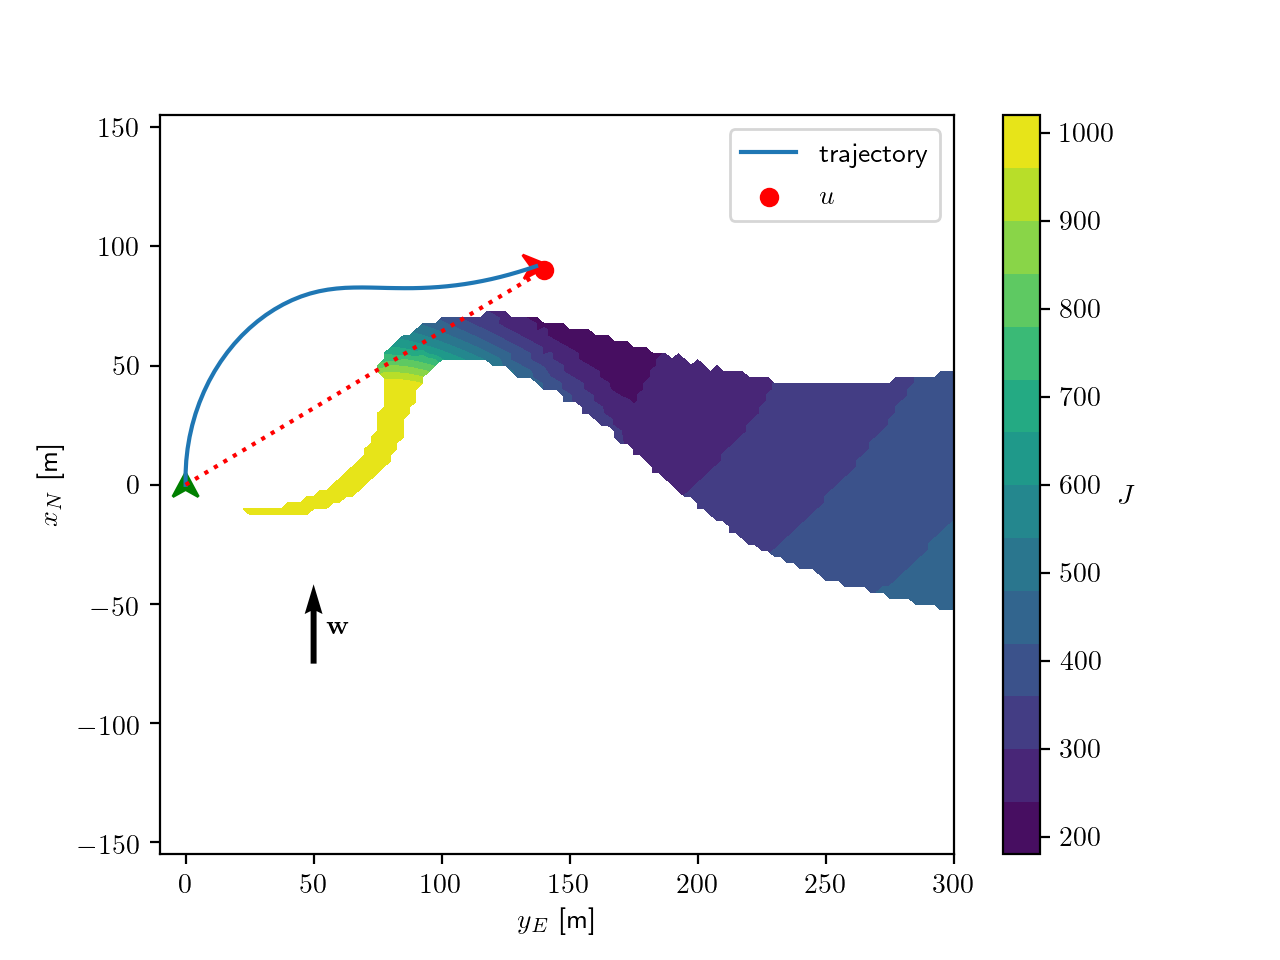
\includegraphics[width=.8\linewidth]{J_sim_90_140}
    \caption{$u=(90,140)$: Infeasible solution due to incorrect final $\cog$.}
    \label{fig:opt_contour_1}
\end{figure}

\begin{figure}[H]
    \centering
    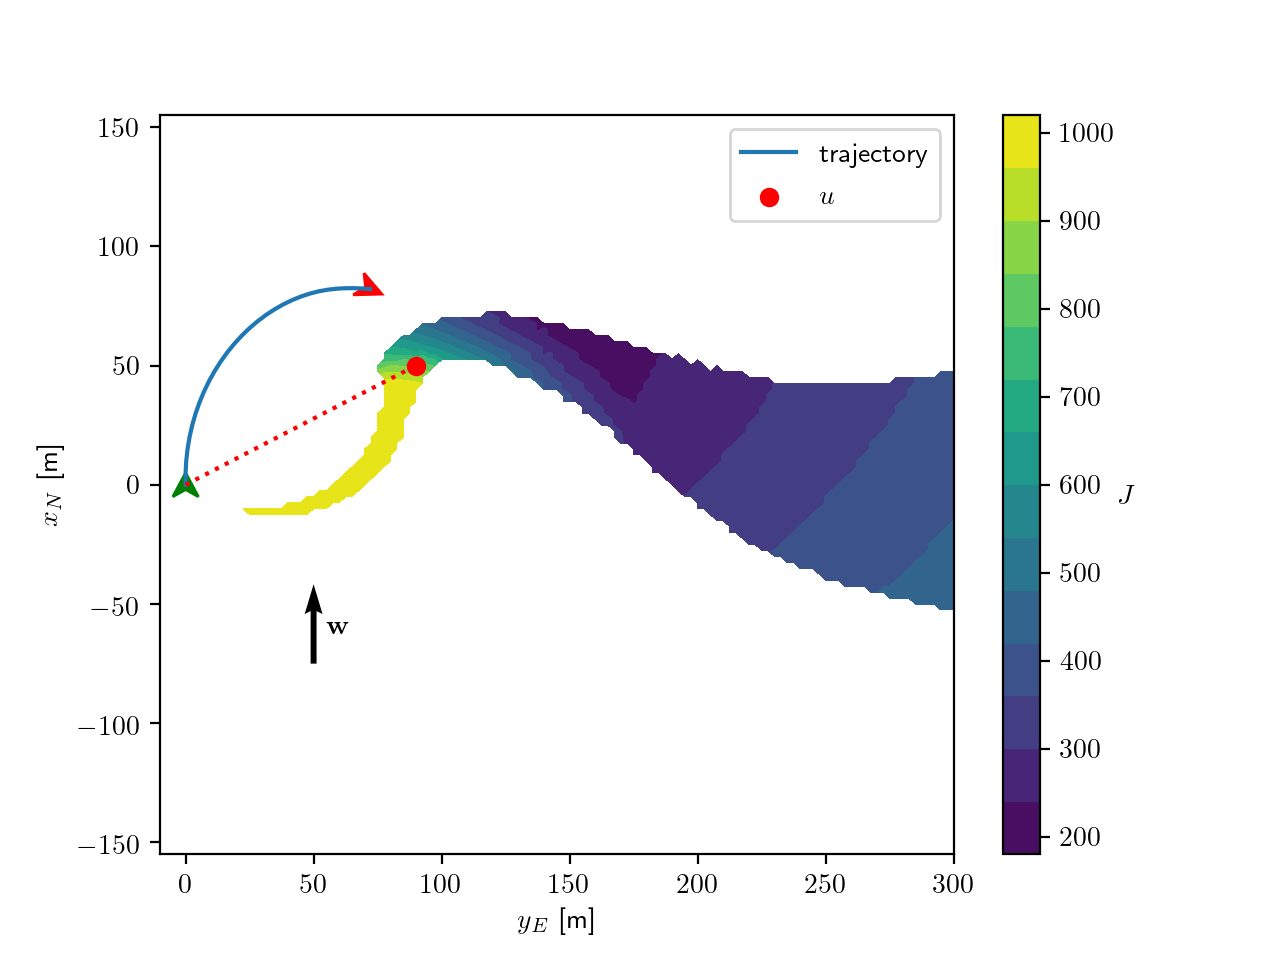
\includegraphics[width=.8\linewidth]{J_sim_50_90}
    \caption{$u=(50,90)$: Sub-optimal solution due to large final cross-track error, $J=891$.}
    \label{fig:opt_contour_2}
\end{figure}

\begin{figure}[H]
    \centering
    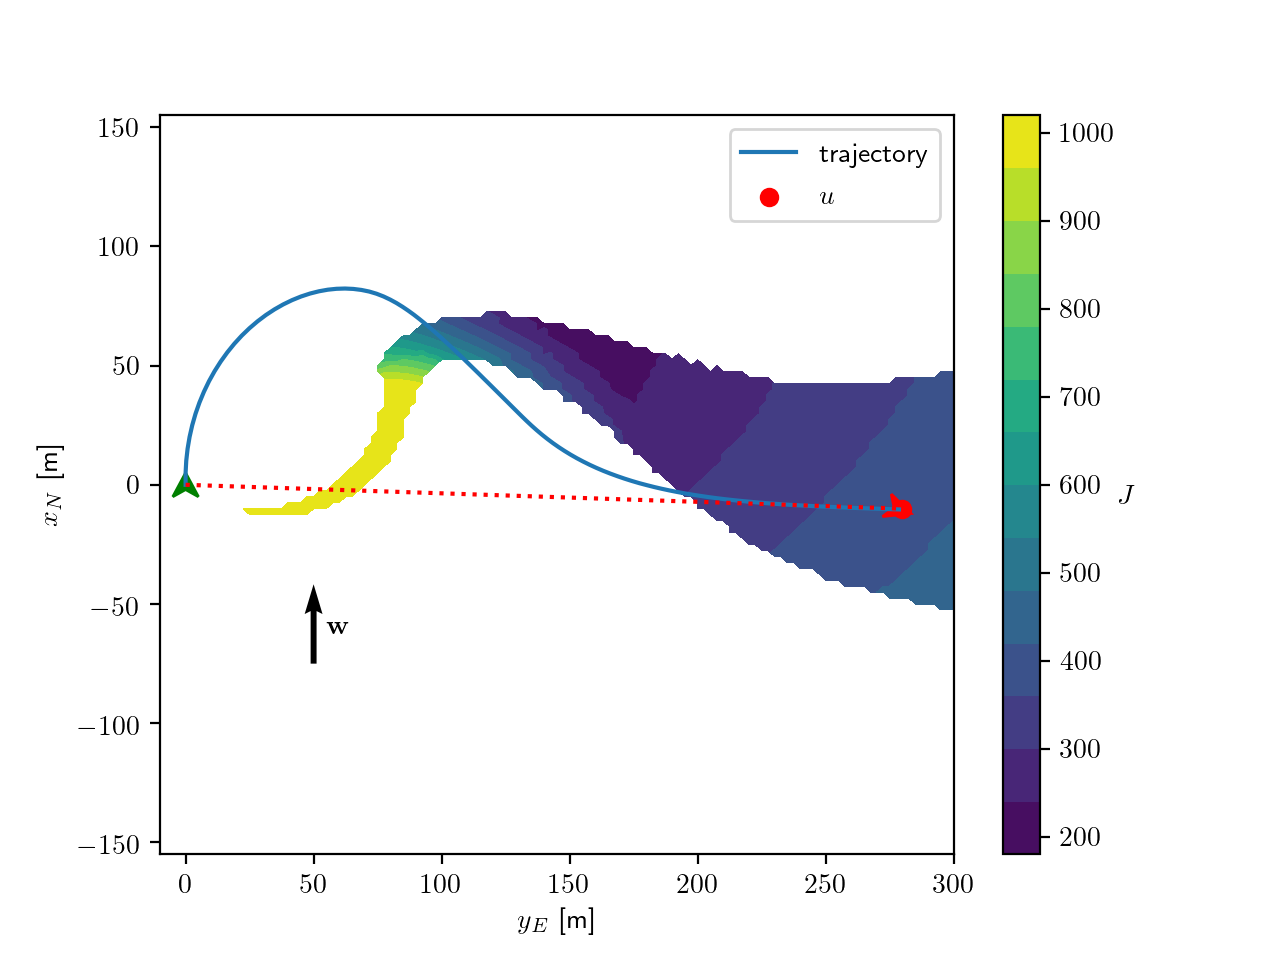
\includegraphics[width=.8\linewidth]{J_sim_10_280}
    \caption{$u=(-10,280)$: Sub-optimal solution due to unnecessarily long trajectory, $J=378$.}
    \label{fig:opt_contour_3}
\end{figure}

\begin{figure}[H]
    \centering
    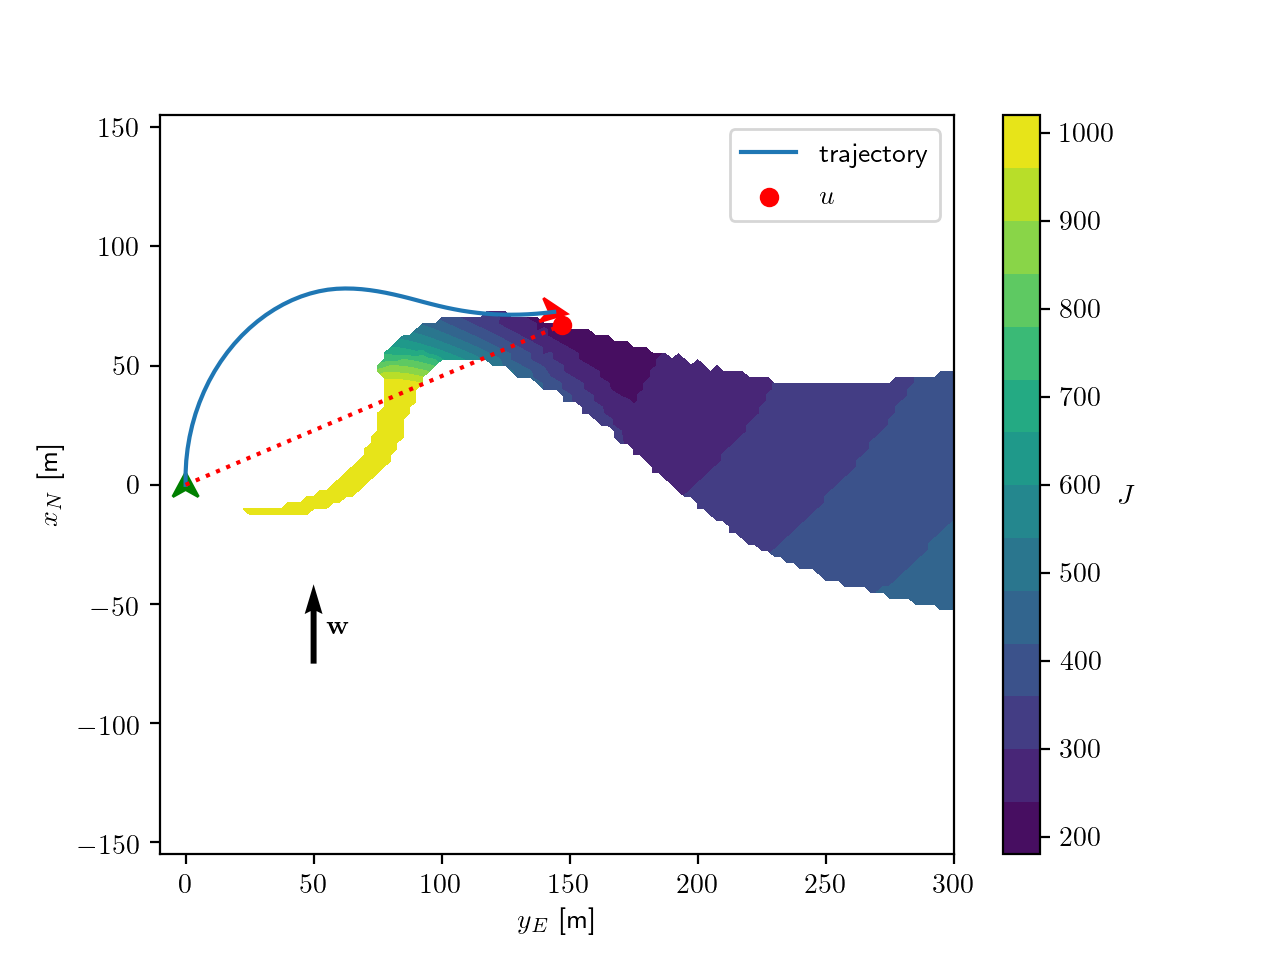
\includegraphics[width=.8\linewidth]{J_sim_67_147}
    \caption{$u=(67,147)$: Optimal solution, $J=186$.}
    \label{fig:opt_contour_4}
\end{figure}

Since there are only two free parameters, the north and east coordinates of $u$, an approximate optimum could be found by performing a grid search over different values of these parameters. However, this solution would depend on the discretization interval of the grid 
and searching over a grid with sufficiently fine resolution is computationally expensive.
A more efficient method is to use \textit{derivative-free} optimization methods, as presented in \cite{derivative_free_opt}. 
In those methods the optimization problem is formulated as 
\begin{subequations}
    \label{eq:derivative_free_opt}
    \begin{alignat}{3}
    &\min_{\xi\in\reals^n}        &\qquad& F: \xi \rightarrow \reals & \\
    &\text{subject to} & & \xi\in\Omega\subseteq \reals^n&\\
    \end{alignat}
\end{subequations}
where no other information, such as the derivatives of $F$, is available.
One class of derivative-free methods called \ac{mads} was introduced in \cite{mads}. This method is based on creating an increasingly fine grid around the currently optimal 
solution on which the objective function is evaluated. In \cite{mads} this method is shown to successfully converge to the global optimum of various non-convex optimization problems using the derivative-free optimization formulation.

\subsection{Robustness during wind variations}
The requirement to generate a set of inputs for each possible wind speed limits 
the practical applicability of the method.
A more useful approach is to generate input sets which handle wind speeds 
$\windspd\in[W_{\text{min}},W_{\text{max}}]$. This problem can be formulated as finding an input $u$ which is feasible for both 
$W_{\text{min}}=(1-\delta_W)\Tilde{\windspd}$ and $W_{\text{max}}=(1+\delta_W)\Tilde{\windspd}$ for some $\delta_W<1$ and $\Tilde{\windspd}=(W_{\text{max}}-W_{\text{min}})/2$. 
To find a solution which is feasible in the extreme cases $\windspd=\windspd_{\text{min}}$ and $\windspd=W_{\text{max}}$, the derivative-free optimization problem was formulated as
\begin{subequations}
    \label{eq:max_opt}
    \begin{alignat}{3}
    &\min_{x, u}        &\qquad& F(x, u)=\max(J_{\text{low}}(x, u),J_{\text{high}}(x, u)) & \\
    &\text{subject to} & & (x, u)\in\Omega &\\
    \end{alignat}
\end{subequations}
where $J_{\text{low}}$ is the value of the objective $J$ in \eqref{eq:opt_problem_mp_uav} for $\windspd=W_{\text{min}}$ and $J_{\text{high}}$ is the value of the objective for $\windspd=W_{\text{max}}$. 
The feasible set $\Omega$ is defined as the values of $x$ and $u$ where the constraints in \eqref{eq:opt_problem_mp_uav} hold for all $\windspd\in[W_{\text{min}},W_{\text{max}}]$.

\section{Improvement step}
As mentioned in Section \ref{sec:hybrid-a-star} the initial solution from Hybrid $A^*$ is often improved using numerical optimization. 
However, due to the limitations presented in Section \ref{sec:solve_opt_ctrl} such methods are not available. Therefore, a simpler and practically motivated approach was used.

The initial solution computed by the Hybrid $A^*$ search is henceforth denoted
\begin{equation}
    \mathcal{M}_{\text{init}}=\{\vec{p}_0,\hdots,\vec{p}_n\}    
\end{equation}
which is an ordered sequence of $n$ waypoints $\vec{p}_i$. A sub-sequence of a mission is denoted
\begin{equation}
    \mathcal{M}_{k:l}=\{\vec{p}_k,\hdots,\vec{p}_l\}, \quad 0\leq k<l\leq n
\end{equation}
A \textit{reduced set} of waypoints is defined as 
\begin{equation}
    \mathcal{M}_{k,l}=\{\vec{p}_k,\vec{p}_l\}
\end{equation}
\ie\ the first and last waypoint of a sub-sequence $\mathcal{M}_{k:l}$. By simulating the closed-loop system using $\mathcal{M}_{\text{init}}$ the inital \ac{cog} and cross-track error $(\cog,d)_i$ at each waypoint can be found. 
Since \eqref{eq:closed_loop} minimizes the cross-track error in each timestep, the following relation always holds:
\begin{equation}
    L(\mathcal{M}_{k:l})\geq L(\mathcal{M}_{k,l})
\end{equation}
where $L(\cdot)$ denotes the length of the trajectory produced by simulating \eqref{eq:closed_loop} with a given waypoint sequence. If the same \ac{cog} and cross-track error 
is achieved and there are no collissions with obstacles while using $\mathcal{M}_{k,l}$ the intermediate waypoints of $\mathcal{M}_{k:l}$ can be eliminated. This method is outlined in Algorithm \eqref{alg:imp} where 
the function $\text{SIMULATE}(\mathcal{M},\xobst)$ returns the \ac{cog} and cross-track error achieved by simulating $\mathcal{M}$ and if there were any 
collissions with $\xobst$. The result of applying the improvement step to a Hybrid $A^*$ solution is illustrated in Figure~\ref{fig:imp}.

\begin{algorithm}
    \begin{algorithmic}
        \Require Initial mission $\mathcal{M}_{\text{init}}$ and corresponding \ac{cog} and cross-track errors $\{(\cog,d)_i\}$
        \State $\mathcal{M}_{\text{imp}}\gets \{\vec{p}_0\}$
        \State $i\gets 0$
        \While{$i\leq n$}
            \State $j\gets i+1$
            \State $(\vec{p}_{\text{best}},i_{\text{best}})\gets(\vec{p}_j,j)$
            \While{$j\leq n$}
                \State $\cog,d,\text{has\_collided}\gets\text{SIMULATE}(\mathcal{M}_{i,j}, \xobst)$
                \If{\textbf{not} has\_collided \textbf{and}$|\cog-\psi_{\text{cog},j}|\leq\Delta\psi_{\text{min}}$ \textbf{and} $|d-d_j|\leq d_{\text{min}}$}
                    \If{j==n}
                        \State $\mathcal{M}_{\text{imp}}\gets \mathcal{M}_{\text{imp}} \bigcup \{\vec{p}_j\}$
                        \State \textbf{return} $\mathcal{M}_{\text{imp}}$
                    \EndIf
                    \State $(\vec{p}_{\text{best}},i_{\text{best}})\gets(\vec{p}_j,j)$
                \EndIf
            \EndWhile
            \State $\mathcal{M}_{\text{imp}}\gets \mathcal{M}_{\text{imp}} \bigcup \{\vec{p}_j\}$
            \State $i\gets i_{\text{best}}$
        \EndWhile 
    \end{algorithmic}
    \caption{Solution improvement by waypoint elimination}
    \label{alg:imp}
\end{algorithm}

\begin{figure}
    \begin{center}
        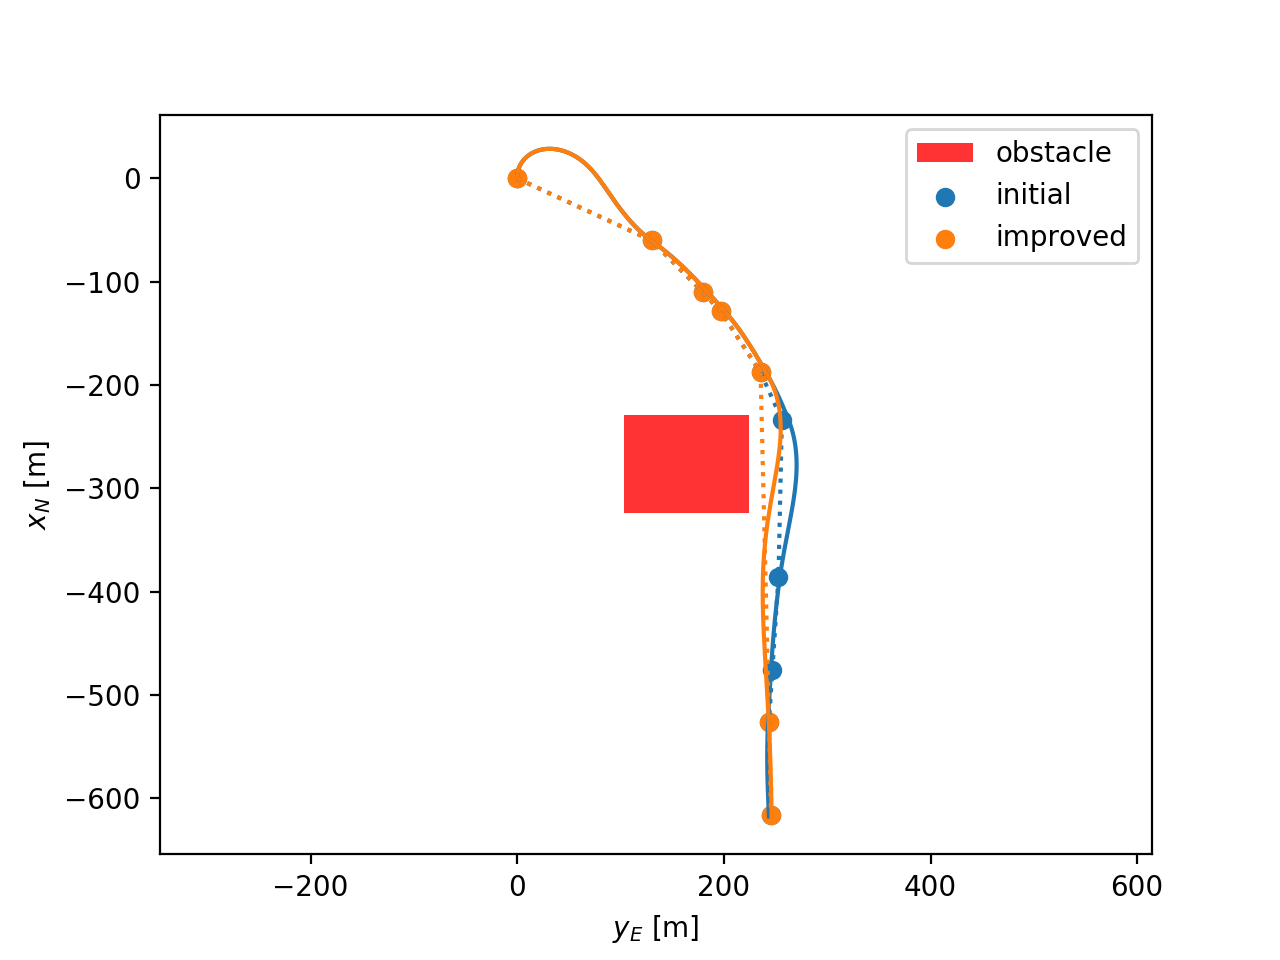
\includegraphics[width=\linewidth]{fig/sol_improved}
        \caption{Trajectory length reduction by eliminating waypoints. $x_0=(0,0,0\degree)$, $x_g=(-615, 245, 180\degree)$. By eliminating the intermediate waypoints in the sub-mission $\mathcal{M}_{4:8}$ the same goal state is reached but the trajectory length is reduced.}
        \label{fig:imp}
    \end{center}
\end{figure}

\section{Heuristic function}
As discussed in Section \ref{sec:a-star}, the choice of heuristic function is 
crucial in achieving good performance of the planner. The goal of the heuristic function is to estimate the 
length of the shortest path relative to the air from an initial state $x_0$ to a final state $x_g$.

\subsection{Cost estimation for straight line-segments}\label{sec:straight_path_heuristic}
Assuming that the heading $\psi$ has converged to $\wca$, the speed of the \ac{uav} 
along a straight line-segment in the inertial frame is given by 
\begin{equation}
    V_{\parallel}=\cos\psi_s(\airspd\cos\wca+\windspd\cos\winddir) + \sin\psi_s(\airspd\sin\wca+\windspd\sin\winddir)
\end{equation}
where $\psi_s$ is the direction defined by the line. This means that the time it takes for the \ac{uav} to travel along the line is equal to 
\begin{equation}
    t=\frac{\|\vec{p}_{i+1}-\vec{p}_i\|}{V_\parallel}
\end{equation}
where $\vec{p}_{i}$ and $\vec{p}_{i+1}$ are the start and end waypoints of the line. Thus, the distance 
travelled relative to the air is equal to 
\begin{equation}
    s_a=V_at=\frac{\airspd}{V_\parallel}\|\vec{p}_{i+1}-\vec{p}_{i}\|
\end{equation}
and $s_a$ provides a good heuristic estimate for traveling along a straight line-segment in wind assuming that $\psi_0=\psi_g=\wca$.
This also implies that the Euclidean distance $\|\vec{p}_{i+1}-\vec{p}_{i}\|$ is not an admissible heuristic if 
$\airspd/V_\parallel<1$.

\subsection{Cost estimation for arbitrary initial and final heading}
Estimating the cost for traveling between states with arbitrary $\psi_0$ and $\psi_g$ is a more challenging problem than straight line-segments.
Methods to calculate such time-optimal paths in the presence of wind are given in both \cite{optimal_path_target} and \cite{optimal_path_trochoidal}, 
but since there is no general analytical solution these methods rely on numerical root-finding techniques.
Solving for roots numerically every time an heuristic estimate is needed was deemed infeasible due to the high computational cost.

When the heuristic cannot be calculated in real-time, an option is to use a \ac{hlut} as discussed in Section \ref{sec:hlut}. By using the generated 
inputs $\inputs$ when calculating costs stored in the \ac{hlut}, these directly correspond to the true cost-to-go. However, a drawback of 
using a \ac{hlut} is that the wind speed $\windspd$ affects the cost, and thus different values of $\windspd$ require different \acp{hlut}. 

To estimate the cost of queries not stored in the \ac{hlut}, these queries can be projected as shown in Figure \ref{fig:hlut_proj}. The total heuristic value can then be estimated as 
\begin{equation}
    \tilde{h}(x, x_g) = h_{\ac{hlut}}(x, x_p) + h_s(x_p, x_g)
\end{equation}
where $h_s(x, \tilde{x})$ is the estimated cost for a straight line-segment.
\begin{figure}
    \begin{center}
        \begin{tikzpicture}
            \draw (-2, -2) rectangle (2, 2);

            \draw[my_v] (0,0) -- node[at end, below]{$y_E$} (1,0);
            \draw[my_v] (0,0) -- node[at end, left]{$x_N$} (0,1);

            \node[point] at (0,0){};
            \node[below] at (0,0){$x$};

            \node[point] at (2,1){};
            \node[above] at (2,1){$x_p$};
            \draw (0,0) -- node[midway, below, anchor=north west]{$h_{\ac{hlut}}(x, x_p)$} (2,1);

            \node[point] at (4,2){};
            \node[above] at (4,2){$x_g$};
            \draw[dashed] (2,1) -- node[midway,below, anchor=north west]{$h_s(x_p,x_g)$} (4,2);

            \node[anchor=west] at (-1.8,-1.75){\ac{hlut} available};
        \end{tikzpicture}
    \end{center}
    \caption{Projection of queries on \ac{hlut}}
    \label{fig:hlut_proj}
\end{figure}

\subsection{Wind variation effects on the heuristic}
If the actual wind speed $\tilde{\windspd}$ is different from the wind speed $\windspd$ used during planning, this 
might affect the admissibility of the heuristic. 
To study this effect, consider traveling along a straight path segment of length $\Delta s=\|x-\tilde{x}\|$ under the assumptions in Section \ref{sec:straight_path_heuristic}. 
An admissible heuristic is then 
\begin{equation}
    \tilde{h}(x, \tilde{x})=\frac{\airspd}{V}\Delta s
\end{equation}
where $V$ is the velocity in the inertial frame. Wind has the largest effect on $V$ when traveling in direct tailwind or headwind, and in those cases $V=\airspd\pm \tilde{\windspd}$. The 
heuristic function $h(x, \tilde{x})$ used during planning is the same but with $V=\airspd\pm \windspd$. The ratio between the admissible and actual heuristics becomes
\begin{equation}\label{eq:wind_heuristic_eps}
    \epsilon = \frac{h}{\tilde{h}} = \frac{\airspd \pm \tilde{\windspd}}{\airspd \pm \windspd}
\end{equation}
where the signs in the numerator and denominator are always equal. As mentioned in Section \ref{sec:sub_optimal} the heuristic is not admissible if 
$\epsilon>1$ which is the case if $\tilde{\windspd}>\windspd$ when traveling in tailwind, or $\tilde{\windspd}<\windspd$ when traveling in headwind.
In these cases, using this heuristic estimate is analouge to using an inflated heuristic with inflation factor $\epsilon$. Moreover, the effects of using an incorrect wind estimate will be more significant if the 
magnitude of $\tilde{\windspd}$ is close to that of $\airspd$.
\chapter{Robust landing sequences}\label{cha:landing}
\section{Problem formulation}
The problem of landing a fixed-wing \ac{uav} on a runway was studied in many previous works, \eg \cite{emergency_landing} and \cite{landing_on_vehicle}. However, small and light-weight \acp{uav} such as the ones studied 
in this thesis can land in any area as long as the ground is flat enough. The main issue is instead that there might be obstacles such as trees around the landing area which limit the possible 
approach directions. Wind also plays an essential role, since landing in tailwind enables much shorter approach paths relative to the ground.

\begin{figure}
    \begin{center}
        \begin{tikzpicture}
            \coordinate (center) at ($(1,1)+(20:1.5)+(110:0.5)$);
            \coordinate (a) at ($(center)+(-130:2)$);
            \draw[fill=lightgray, rotate around={20:(1,1)}] (1,1) rectangle (4,2);
            \draw[](0,1) -- ++ (80:1.5) -- ++ (20:1) -- ++ (45:0.75) -- (0,4) --++ (-2, -1.5) -- (-1,1) -- (0,1);
            \node at (-.5,2.5){$\xobst$};
            \node at ($(center)+(-160:1)$){$\landing$};
            \draw (center) -- ++ (-130:2);
            \node[point] at (center){};
            \node[above] at (center){$\vec{p}_L$};
            \node[point] at (a){};
            \node[below] at (a){$\vec{p}_A$};
            \draw[my_v] ($(center)+(20:3)$) -- node[above]{$\windvec$} ++ (-1,0);
            \Drone{-1}{0}{10}
            \draw[dashed](-1,0) -- (a);            
        \end{tikzpicture}
    \end{center}
    \caption{Landing sequence definition}
    \label{fig:land}          
\end{figure}

The problem of landing is thus defined as finding the inputs which lands the \ac{uav} as close to the center as possible in a pre-defined landing area $\landing$. The landing area is 
defined as a rectangular region with walls of height $h_{\text{safe}}$, and to ensure safe landing the \ac{uav} must enter $\landing$ above this altitude. 
There might also be obstacle regions $\xobst$ around the landing area where the \ac{uav} is not permitted to fly. The problem definition is illustrated in Figure \ref{fig:land}.

\section{Landing sequence}
A landing sequence for fixed-wing \acp{uav} is defined by an approach point $\vec{p}_A$ and landing point $\vec{p}_L$. These points 
define an approach direction $\psi_L$. The landing velocity $V_L$ depends on $\psi_L$, the airspeed $\airspd$ and current wind as 
\begin{equation}
    V_L=\cos\psi_L(\airspd\cos\wca+\windspd\cos\winddir) + \sin\psi_L(\airspd\sin\wca+\windspd\sin\winddir)
\end{equation}
The landing sequence is divided into an approach phase and a flare phase, which are illustrated in Figure \ref{fig:land_alt}.
During the approach phase, the autopilot commands an approach sink-rate
\begin{equation}\label{eq:sink_rate}
    \dot{h}_{cmd}=\frac{h_0-\flarealt}{\|\vec{p}_A-\vec{p}_L\|-R_{\text{flare}}}V_L
\end{equation}
where $h_0$ is the initial altitude, $\flarealt$ is the flare altitude and $R_{\text{flare}}$ is the flare distance.
To ensure smooth landing, the flare phase is activated once the \ac{uav} reaches the altitude $\flarealt$ above the ground. 
In this mode it instead tries to achieve a pre-defined flare sink-rate 
\begin{equation}
    \dot{h}=\flaresink
\end{equation}
which means that the flare distance is given by
\begin{equation}\label{eq:R_flare}
    R_{\text{flare}}=\flarealt\frac{V_L}{\flaresink}
\end{equation}
Due to physical limitations in the system, the landing sequence has to be defined such that 
\begin{equation}\label{eq:sink_constraint}
    \dot{h}_{cmd}\leq\dot{h}_{\text{max}}
\end{equation}
for some constant $\dot{h}_{\text{max}}$ during the approach.

\begin{figure}
    \begin{center}
        \begin{tikzpicture}
            \draw[-|] (0,0) -- node[at end, left]{$h_0$} (0,5);
            \draw[-|] (0,0) -- node[at end, left]{$\flarealt$} (0,1);
            \draw (0,0) -- (7,0);

            \draw[dashed] (0,5) -- node[midway, anchor=200]{Approach} (4,1);
            \draw[dashed] (4,1) -- node[midway, anchor=200]{Flare} (7,0);
            \draw[dotted] (0,1) -- (4,1);

            \draw[blue] (0,5) .. controls (4,1) and (4,1) .. (7,0);
        \end{tikzpicture}
    \end{center}
    \caption{Altitude profile of a fixed-wing landing sequence}
    \label{fig:land_alt}
\end{figure}

\section{Calculating a landing sequence}
The goal of the landing sequence generation is to ensure safe landing in the specified area $\landing$. There are two important measures to 
discuss regarding the safety of a landing sequence, the altitude of the \ac{uav} when entering $\landing$ and the distance from the landing point to the center of $\landing$. 
If the entry altitude is too low, there is a risk of colliding with surrounding obstacles and if the distance to the center is too large, the \ac{uav} will not land in the designated area. 
Thus, by minimizing these two errors the safety of the landing sequence is maximized. This also maximizes the robustness to other errors such as 
variations in wind speed.

Since a partial goal of the landing sequence is to land as closely as possible to the center point $\vec{p}_c$ of the landing area $\landing$, any 
landing sequence is defined by placing $\vec{p}_A$ and $\vec{p}_L$ along a line which passes through $\vec{p}_C$ and points in the direction given by $\psi_L$.
This fact can be used to divide the problem in two parts, where first the best $\psi_L$ is determined and then $\vec{p}_A$ and $\vec{p}_L$ based on the chosen direction.

\begin{figure}
    \begin{center}
        \begin{tikzpicture}
            \coordinate (center) at (2,1);
            \coordinate (p1) at ($(center)+(-1.5,-1)$);
            \coordinate (p2) at ($(center)+(1.5,1)$);
            \coordinate (pa) at ($(p1)+(-.75,-.5)$);
            \coordinate (pl) at ($(center)+(.75,.5)$);

            \draw[fill=lightgray] (0,0) rectangle (4,2);
            \node[point] at (p1){};
            \node[below] at (p1){$\vec{p}_1$};

            \node[point] at (p2){};
            \node[above] at (p2){$\vec{p}_2$};

            \node[point] at (center){};
            \node[above] at (center){$\vec{p}_c$};

            \draw[dashed] ($(p1)+(-3,-2)$) -- (p2);
            \node[below] at (pa){$\vec{p}_A$};
            \node[point] at (pa){};

            \node[above] at (pl){${\vec{p}_L}$};
            \node[point] at (pl){};

            \draw[line width=1.5pt] (pa) -- (pl);

            \Drone{-2.5}{-2}{30};
            \draw[dashed] ($(-2.5,-2)+(.75,.5)$) -- ++ (1,0);
            \draw ($(-2.5,-2)+(1.25,.5)$) arc(0:30:.5) node[midway, anchor=200]{$\psi_L$};

            \node at (3.5,.5){$\landing$};
            \draw[my_v] (2, 4) -- node[left]{$\windvec$} ++ (0,-1);
        \end{tikzpicture}
    \end{center}
    \caption{Variables determining a landing sequence}
    \label{fig:opt_landing}
\end{figure}

\subsection{Determining the approach direction}
Any line through $\vec{p}_c$ with a given direction will cross the walls of $\landing$ in exactly two points $\vec{p}_1$ and $\vec{p}_2$, as is illustrated in Figure \ref{fig:opt_landing}. 
We thus have the following constraints to consider:
\begin{itemize}
    \item The distance $\|\vec{p}_1-\vec{p}_2\|$ has to be large enough such that the altitude $h$ in $\vec{p}_1$ is larger than $h_{\text{safe}}$ while allowing 
    the constraint \eqref{eq:sink_constraint} to be satisfied
    \item The approach direction $\psi_L$ has to be chosen such that the initial trajectory up until $\vec{p}_A$ is not inside $\xobst$
\end{itemize}
To find the minimum feasible distance, the altitude of the \ac{uav} when entering $\landing$ is denoted $h_A$.
Assuming that $h_A=h_{\text{safe}}$, the minimum feasible distance to the flare point is given by
\begin{equation}
    R_{\text{min}}=(h_{\text{safe}}-\flarealt)\frac{V_L}{\dot{h}_{\text{max}}}
\end{equation}
To ensure landing in $\landing$ it is thus required that 
\begin{equation}
    \|\vec{p}_1-\vec{p}_2\|\geq R_{\text{min}}+R_{\text{flare}}
\end{equation}
where $R_{\text{flare}}$ is given by Equation \eqref{eq:R_flare}. To ensure the second constraint, a simple approach is to 
create lines starting in $\vec{p}_c$ with length $K(R_{\text{min}}+R_{\text{flare}})$ and direction $\psi_L+180\degree$ for some $K\geq0.5$ and different discrete values of $\psi_L$. 
The set of feasible approach directions $\{\psi_{L}\}_{\text{feas}}$ can then be found by checking each corresponding line for intersections with $\xobst$. Finally, the approach direction is 
chosen as 
\begin{equation}
    \psi_{L}^* = \argmin_{\psi\in\{\psi_{L}\}_{\text{feas}}}R(\psi)
\end{equation}
where
\begin{equation}
    R(\psi)=R_{\text{min}}(\psi) + R_{\text{flare}}(\psi)
\end{equation}

\subsection{Determining the approach points}
After fixing the approach direction to $\psi_L=\psi_{L}^*$ the next step is to calculate the values of $\vec{p}_A$ and $\vec{p}_L$. 
Since the approach direction is fixed, the remaining variables can be redefined as 
\begin{subequations}
    \begin{align}
        R_a&=(\vec{p}_A-\vec{p}_2)\cdot\hat{l}\\
        R_l&=(\vec{p}_L-\vec{p}_2)\cdot\hat{l}
    \end{align}
\end{subequations}
where $\hat{l}$ is a unit vector pointing in the direction $\psi_L+180\degree$. This definition ensures landing in $\landing$ as long as $0\leq R_l\leq 2R_c$, where
\begin{equation}
    R_c=\|\vec{p}_1-\vec{p}_2\|/2
\end{equation} 
The problem is thus finding $R_a$ and $R_l$ so that $|h_A-h_{\text{safe}}|$ is maximized and $|R_c-R_l|$ is minimized, while fulfilling the given constraints.
From Equation \eqref{eq:sink_rate}, the commanded sink-rate is then
\begin{equation}
    \dot{h}_{\text{cmd}}=\frac{h_0-\flarealt}{R_a-R_l-R_{\text{flare}}}V_L
\end{equation}
and the altitude during the approach is given by
\begin{equation}
    h(R) = h_0 - R\frac{\dot{h}_{\text{cmd}}}{V_L}=h_0-R\frac{h_0-\flarealt}{R_a-R_l-R_{\text{flare}}}
\end{equation}
where $h_0$ is the initial altitude. To ensure enough altitude when entering $\landing$, it is required that
\begin{equation}\label{eq:h_a_constraint}
    h_A=h(R_a-2R_c)\geq h_{\text{safe}}
\end{equation}
The landing parameters can thus be calculated by solving the optimization problem
\begin{subequations}
    \label{eq:opt_problem_land}
    \begin{alignat}{3}
    &\min_{R_a,R_l}        &\qquad& J=|R_c-R_l|^2 - |h_A-h_{\text{safe}}|^2 & \\
    &\text{subject to} & & 0\leq R_l \leq 2R_c &\\
    & & & \dot{h}_{\text{cmd}}=\frac{h_0-\flarealt}{R_a - R_l - R_{\text{flare}}}V_L\\
    & & & h_A = h_0 - \frac{R_a - 2R_c}{R_a - R_l - R_{\text{flare}}}(h_0-\flarealt)\\
    & & & \dot{h}_{\text{cmd}}\leq \dot{h}_{\text{max}}\\
    & & & h_A\geq h_{\text{safe}}\\
    \end{alignat}
\end{subequations}

This is a non-linear optimization problem with linear constraints, which can be solved with methods such as \ac{ipopt} \cite{ipopt}.

\chapter{Implementation}\label{cha:implementation}
\section{System overview}
An overview of the proposed system is shown in Figure \ref{fig:sys_overview}.
\begin{figure}
    \begin{center}
        \begin{tikzpicture}[node distance = 3cm, auto]
            \node[block] (init){Landing area input};
            \node[block, right of=init] (land){Landing sequence calculation};
            \node[block, below of=land] (obst){Obstacle database};
            \node[block, above of=land] (wind){Wind estimation};
            \node[block, right of=land] (mp){Motion planner};
            \node[block, above of=mp] (gps){Positioning system};
            \node[block, right of=mp] (traj){Waypoint controller};

            \path[line] (init) - > node{$\mathcal{A}$} (land); 
            \path[line] (obst) - > node[midway, right]{$\mathcal{X}_{obst}$} (land);
            \path[line] (obst) - > node[midway, right]{$\mathcal{X}_{obst}$} (mp);
            \path[line] (wind) - > node[midway, right]{$\vec{w}$} (land);
            \path[line] (wind) - > node[midway, right]{$\vec{w}$} (mp);
            \path[line] (land) - > node[midway]{$x_f$} (mp);
            \path[line] (gps) - > node[midway, right]{$x_i$} (mp);
            \path[line] (mp) - > node[midway]{$\mathcal{M}$} (traj);
        \end{tikzpicture}
    \end{center}
    \caption{System overview}
    \label{fig:sys_overview}
\end{figure}
The UAV is assumed to be equipped with a wind estimation system which can observe the current wind vector $\vec{w}$, and a positioning system which delivers the current position of the UAV. 
There is also an obstacle database which contains the zones $\mathcal{X}_{obst}$ where the UAV is not allowed to fly. The user inputs a desired landing area $\mathcal{A}$ which is 
used to calculate an optimal landing sequence as described in Chapter \ref{cha:landing}. The resulting optimal approach point is sent as the final state to the motion planner, which calculates a plan from the current 
position received from the positioning system. This plan is then transformed to a waypoint mission $\mathcal{M}$ which is sent for execution to the waypoint controller.
\section{Simulation environment}
The implementation is based on the Ardupilot Software-In-The-Loop (SITL) environment \cite{ardupilot_sitl}. This simulation environment is based on the 
JSBSim simulator \cite{jsbsim}, and is capable of simulating both constant and time-varying wind. The default simulation model is based on the 
Rascal 110 fixed-wing UAV.
\section{Obstacle avoidance}
To ensure low execution times it is crucial to use an efficient method of checking for collisions between states and $\mathcal{X}_{obst}$. 
In this implementation, the S2Geometry library developed by Google was used \cite{s2geo}. This is a C++ library which contains 
efficient methods to index geometrical objects of any shape, and checking for collisions between different geometries such as points, lines and polygons. 
\section{Wind estimation}
In this thesis the EKF-based wind estimation system described in Section \ref{sec:wind_ekf} was used.
\section{Landing sequence calculation}
In order to calculate the optimal landing sequence the optimization problem \eqref{eq:opt_problem_land} has to be solved. 
This problem was solved using the CasADi toolkit, which is a general toolkit for solving nonlinear optimization problems numerically \cite{casadi}.
\section{Motion planner} 
\subsection{Motion Primitive Generation}
Motion primitives are generated using the approach described in Section \ref{sec:motion_prims_wind}. 
The motion primitive set was generated for wind directions $\psi_{w,d}=\{0\degree,20\degree,40\degree,\hdots340\degree\}$ and desired final course 
$\psi_d=\{10\degree,20\degree,\hdots160\degree\}$, resulting in a total of 284 primitives for a specific wind speed $W$. Symmetries of the system mean that motion primitives 
for $\psi_d=\{-10\degree,-20\degree,\hdots-160\degree\}$ are simply found by mirroring the $p_E$ coordinate of $u$.
The optimization problem was solved using NOMAD \cite{nomad}, a C++ implementation of the MADS algorithm. The initial guess for $u$ was defined as 
\begin{equation}
    u_0=(d\cos\psi_d,d\sin\psi_d)
\end{equation}
for the current value of $\psi_d$ and $d=100$ meters. 
Simulations of the closed-loop system for the optimal inputs $u$ calculated for some different wind directions and $W=5$ m/s are shown in Figure \ref{fig:motion_prims}.
\begin{figure}
    \begin{center}
        \subfloat[$\psi_w=0\degree$]{
            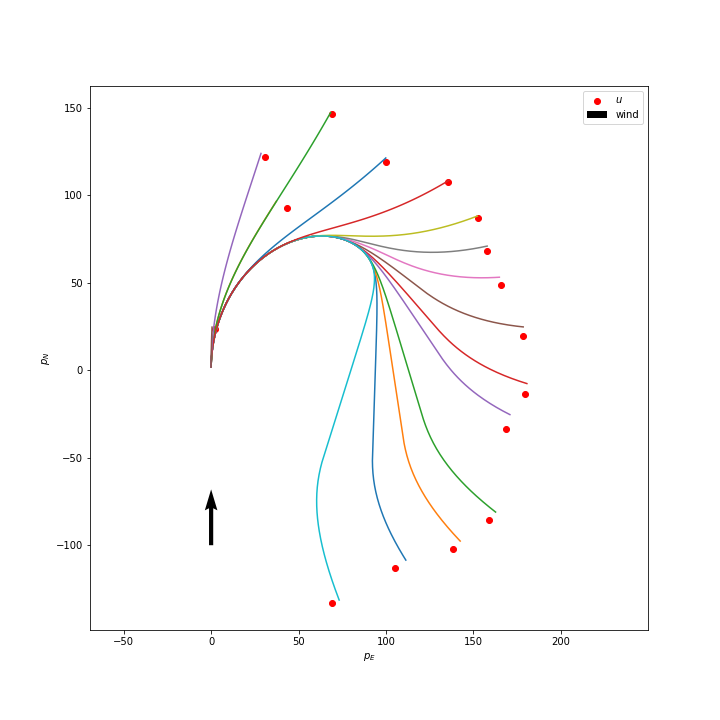
\includegraphics[width=.48\linewidth]{mp_0}
        }
        \subfloat[$\psi_w=160\degree$]{
            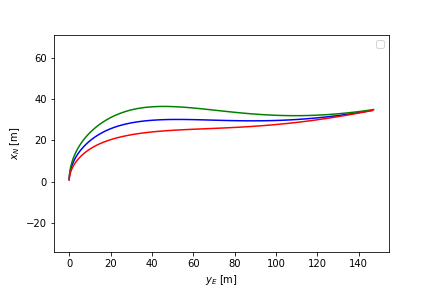
\includegraphics[width=.48\linewidth]{mp_160}
        }
    \end{center}
    \caption{Motion primitives for different wind directions, $W=5$ m/s}
    \label{fig:motion_prims}
\end{figure}

\subsection{State-space discretization}
To apply graph-search methods the state-space has to be discretized. In this work the values of $p_N$ and $p_E$ were discretized into cells of size $d=10$ meters, and the 
yaw angle $\psi$ was discretized in steps of $20\degree$. The Hybrid A-star method was used when sampling the state space, allowing continuous values of the state vector $x$ but assigning those to the closest 
discretized state.

\subsection{State expansions}
The step $\text{EXPAND}(x,\mathcal{P})$ in Algorithm \ref{alg:astar} has to take both the wind direction $\psi_w$ and the heading $\psi$ of $x$ into account. 
Since the motion primitives in $\mathcal{P}$ are generated using initial heading $\psi_i=0$, it is first necessary to calculate the closest relative wind direction
\begin{equation}
    \psi_{w,rel}=\argmin_{\psi_{w,d}\in\{\psi_{w,d}\}}|(\psi-\psi_w)-\psi_{w,d}|
\end{equation}
which is used to select the motion primitives used for expansion. When mirroring primitives the wind direction also has to be mirrored so that 
$\psi_w'=360\degree-\psi_w$. The selected motion primitives also have to be rotated so that the initial reference $u=(p_{N,g},p_{E,g})$ is transformed to 
\begin{equation}
    u'=(\cos\psi p_{N,g} + \sin\psi p_{E,g}, -\sin\psi p_{N,g} + \cos\psi p_{E,g})
\end{equation}
Finally the expanded states and corresponding costs are found by simulating the closed-loop system \eqref{eq:closed_loop} using each selected $u'$ as input. 
In simulation, the actual wind direction $\psi_w$ is used.

\subsection{Heuristic Lookup Table}
The HLUT was generated using the method in Algorithm \ref{alg:hlut}. The HLUT was generated using the wind-direction $\psi_w=0$, which means that 
entries have to be generated for initial values of $\psi$ from $0\degree$ to $180\degree$ to cover all possibilities. To lookup a query $h(x, x')$ it is then 
necessary to rotate both $x$ and $x'$ by the angle $\psi_w$ in order for the query to align with the HLUT. 

To lower the amount of generated entries the discretization grid was increased to $d=20$ meters when constructing the HLUT. The set of 
values for which to generate entries was selected as 
\begin{equation}
    \mathcal{X}=\{(p_N,p_E): |p_N|\leq D \cup |p_E| \leq D\}
\end{equation}
for $D=400$ m. To ensure that HLUT are entries are available for at least states within a smaller set with $D=200$ m, an additional 
A-star search was performed for each missing such state after the initial generation. For $W=5$ m/s the resulting HLUT consists of 235359 entries. 
A plot of the HLUT values for initial and final heading $\psi_i=\psi_f=0\degree$ can be seen in Figure \ref{fig:hlut}. The dark values at the bottom correspond to where there are no HLUT entries available. 

\begin{figure}
    \begin{center}
        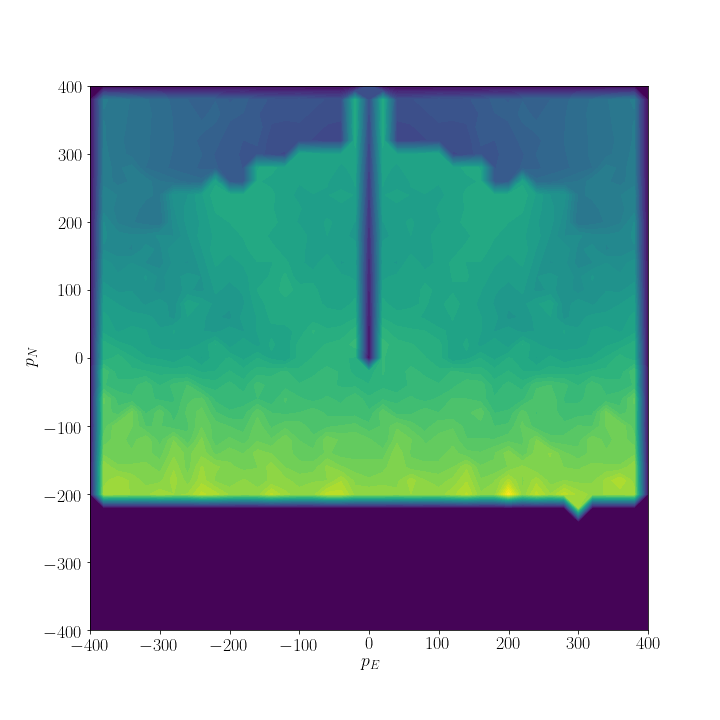
\includegraphics[width=.6\linewidth]{hlut}
    \end{center}
    \caption{HLUT for $W=5$ m/s and $\psi_f=0\degree$}
    \label{fig:hlut}
\end{figure}

\section{Waypoint controller}
To send the calculated motion plan and landing sequence to the waypoint controller, these have to be converted to the 
MAVLink protocol which is supported by the ArduPlane autopilot \cite{mavlink}. This interface was implemented using the MAVROS 
plugin in ROS \cite{mavros}. ROS is a modular framework for robotics applications, with API:s available in both Python and C++ \cite{ros}.

\chapter{Implementation and experiments}\label{cha:results}

\section{Implementation details}
The following sections describe relevant details regarding the implementation of the proposed method.

\subsection{Obstacle avoidance}
To ensure low execution times it is crucial to use an efficient method of checking for collisions between states and $\xobst$. 
In this implementation, the S2Geometry library developed by Google was used \cite{s2geo}. This is a C++ library which contains 
efficient methods to index geometrical objects of any shape, and checking for collisions between different geometries such as points, lines and polygons. 

\subsection{Input set generation}
The input set $\inputs$ was generated using the approach described in Section \ref{sec:motion_prims_wind}. 
It was generated for wind directions $\psi_{w,s}=\{0\degree,20\degree,40\degree,\hdots,340\degree\}$ and desired final course changes
$\Delta\cog=\{20\degree,40\degree,\hdots,180\degree\}$, resulting in a total of 162 inputs for each specific $\windspd$. Symmetries of the system reduce the set of necessary inputs
as solutions for $\Delta\cog=\{-20\degree,-40\degree,\hdots,-180\degree\}$ are simply found by mirroring the $y_E$ coordinate of $u$.
The optimization problem was solved using \textabbr{nomad} \cite{nomad}, a C++ implementation of the \ac{mads} algorithm introduced in Section \ref{sec:solve_opt_ctrl}.
Cross-track error constraints were defined by $\lambda_d=25$ and $d_{\text{min}}=2.5$ m, \ac{cog} error $\Delta\psi=15\degree$ and wind variation $\delta_W=0.25$. The initial guess for $u$ 
was found by performing a grid search over the values
\begin{equation}
    \actions_{s,\text{init}}=\{(\Delta x_N,\Delta y_E): |\Delta x_N| \leq 300, 0\leq \Delta y_N \leq 300\}
\end{equation}
with a step size of 10 meters and selecting the input with the lowest value of the objective in Equation \eqref{eq:max_opt}.
Simulations of the closed-loop system for the generated inputs $u$, calculated for some different wind directions and $\windspd\in[3.75, 6.25]$ m/s, are shown in Figure \ref{fig:motion_prims}.
\begin{figure}
    \centering
    \subfloat[Inputs generated for $\winddir=0\degree$]{
        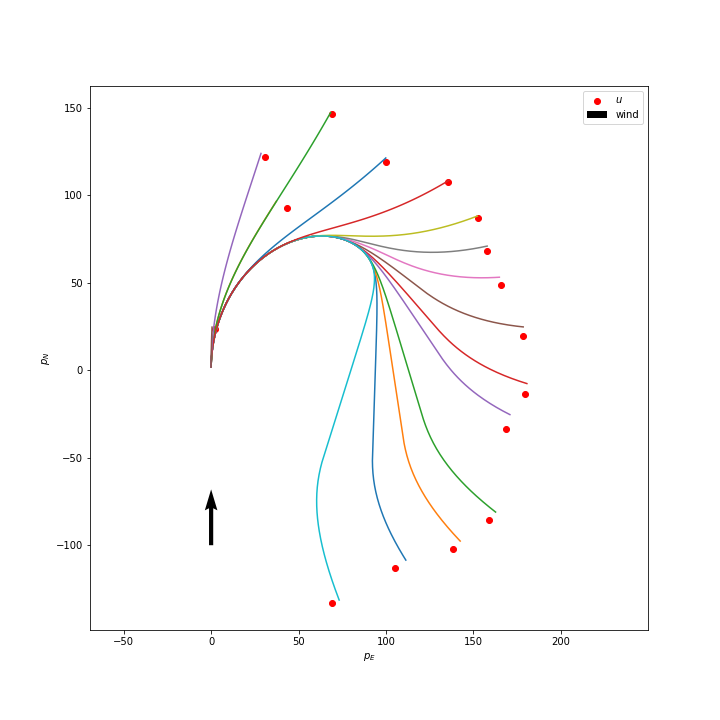
\includegraphics[width=.8\linewidth]{mp_0}
    }\\
    \subfloat[Inputs generated for $\winddir=80\degree$]{
        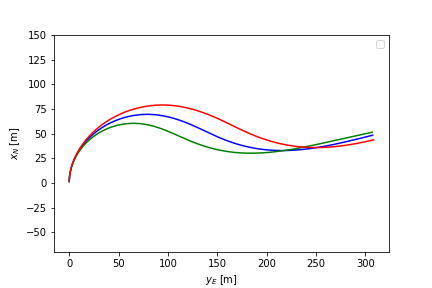
\includegraphics[width=.8\linewidth]{mp_80}
    }
    \caption{Inputs for different wind directions, $\windspd\in[3.75, 6.25]$ m/s}
    \label{fig:motion_prims}
\end{figure}

\subsection{State-space discretization}
To apply graph-search methods, the state-space has to be discretized. In this work the values of $x_N$ and $y_E$ were discretized into cells of size $d=10$ meters, and the 
heading $\psi$ was discretized in steps of $20\degree$. The Hybrid $A^*$ method presented in Section \ref{sec:hybrid-a-star} was used when sampling the state space, allowing continuous values of the state vector $x$ but assigning those to the closest 
discretized state.

\subsection{State expansions}
The step $\text{EXPAND}$ in Algorithm \ref{alg:astar} presented in Section \ref{sec:a-star} has to take both the wind direction $\winddir$ and the heading $\psi$ of $x$ into account. 
Since the inputs in $\inputs$ are generated using initial course $\cog=0$, it is first necessary to calculate the closest relative wind direction
\begin{equation}
    \psi_{w,\text{rel}}=\argmin_{\psi_{w,s}\in\{\psi_{w,s}\}}|(\psi-\winddir)-\psi_{w,s}|
\end{equation}
which is used to select the inputs for expansion. When mirroring inputs the wind direction also has to be mirrored, \ie\ 
$\tilde{\psi}_w=360\degree-\winddir$ is used to calculate $\psi_{w,\text{rel}}$. The selected inputs also have to be rotated, \ie\ the initial reference $u=(\Delta x_N, \Delta y_E)$ is transformed to 
\begin{equation}
    \tilde{u}=(\cos\psi \Delta x_N + \sin\psi \Delta y_E, -\sin\psi \Delta x_N + \cos\psi \Delta y_E)
\end{equation}
Finally, the expanded states and corresponding costs are found by simulating the closed-loop system \eqref{eq:closed_loop} using each selected $\tilde{u}$ as input. 
The actual wind direction $\winddir$ is used instead of $\psi_{w,s}$ in these simulations.

\subsubsection{Handling perpendicular winds}
A drawback of using straight line-segments as the control reference is that some inputs become problematic when the difference between 
$\psi$ and $\winddir$ is close to $90 \degree$. In this situation, expanding using an input which corresponds to a course change 
 of $\Delta\cog\approx180\degree$ might result in the trajectory controller choosing to fly in tailwind instead of headwind, leading to a large cross track error. This situation is 
 illustrated in Figure \ref{fig:hdg_diff_wind}.

\begin{figure}
    \begin{center}
        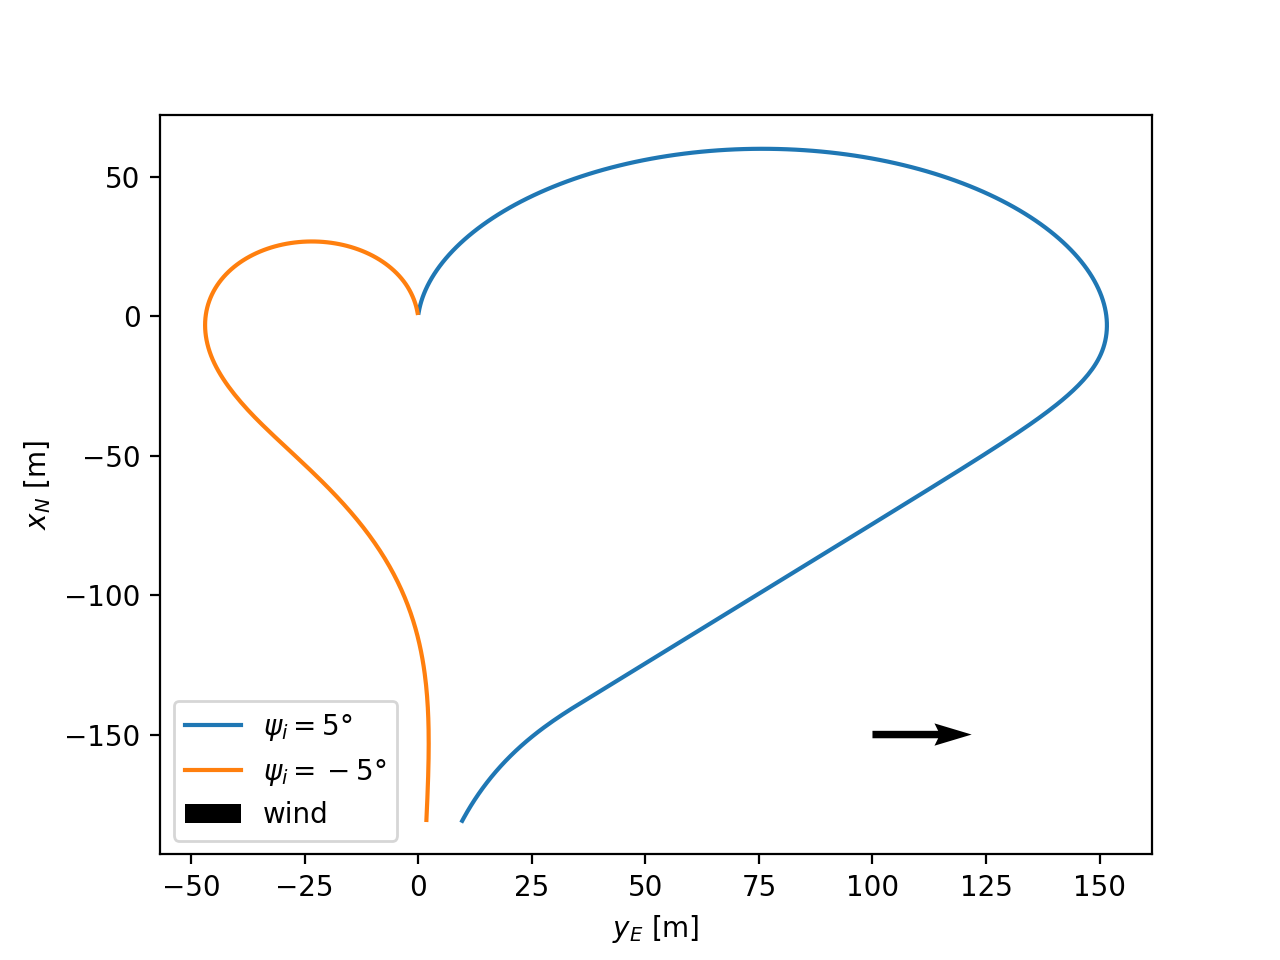
\includegraphics[width=.7\linewidth]{fig/prim_diff_hdg}        
    \end{center}
    \caption{Large cross track error for $\Delta\cog\approx180\degree$ when the wind is perpendicular to \ac{uav} motion}
    \label{fig:hdg_diff_wind}
\end{figure}

This issue was mitigated by defining a set $\psi_{\text{safe}}$ as 
\begin{equation}
    \psi_{\text{safe}}=\{\psi: |\sin\psi|<\frac{1}{\sqrt{2}}\}
\end{equation}
If $|\psi-\winddir|\notin\psi_{\text{safe}}$ during expansion only inputs corresponding to $|\Delta\cog|\leq160\degree$ are used.

\subsection{Heuristic Lookup Table}
The \ac{hlut} was generated using the method in Algorithm \ref{alg:hlut} presented in section \ref{sec:hlut}, using the wind-direction $\winddir=0$. This implies that 
entries have to be generated for initial values of $\psi$ from $0\degree$ to $180\degree$ to cover all possible situations. To query a stored heuristic value $\tilde{h}(x, \tilde{x})$ it is 
thus necessary to rotate both $x$ and $\tilde{x}$ by the angle $\winddir$ in order for the query to align with the \ac{hlut}. 

The set of states for which to generate entries was selected as 
\begin{equation}
    \states=\{(x_N,y_E): |x_N|\leq D \cup |y_E| \leq D\}
\end{equation}
for $D=400$ m. To ensure that \ac{hlut} entries are available for at least states within a smaller set with $D=200$ m, an additional 
$A^*$ search was performed for each such missing state after the initial generation. For $\windspd=5$ m/s the resulting \ac{hlut} consists of 951099 entries.

\subsection{Waypoint controller}
To send the calculated motion plan and landing sequence to the waypoint controller, these have to be converted to the 
MAVLink protocol which is supported by the ArduPlane autopilot \cite{mavlink}. This interface was implemented using the MAVROS 
plugin in \textabbr{ros} \cite{mavros}. \textabbr{ros} is a modular framework for robotics applications, with API:s available in both Python and C++ \cite{ros}.

\subsection{Wind estimation}
In simulated experiments, the wind was assumed to be perfectly estimated, \ie\, the values of $\windspd$ and $\winddir$ configured in the simulator were also passed to the algorithm. 
During real flight experiments, the ArduPilot \ac{ekf} based wind measurement system described in Section \ref{sec:wind_ekf} was used to provide estimates. Since the wind is assumed constant in this work, a \ac{ma} filter with a 
window size of 2 seconds was used to remove small variations in the measurements.

\section{Simulation experiments}
In this section, setup and results of simulation experiments are presented.
\subsection{Experimental setup}
The proposed method was evaluated by performing a number of simulations in the Ardupilot \ac{sitl} environment \cite{ardupilot_sitl}. This environment is based on the 
JSBSim flight dynamics simulator \cite{jsbsim}, and is capable of simulating wind effects. The default simulation model is based on the Rascal 110 fixed-wing \ac{uav} \cite{rascal}.
The parameters used during these simulations are summarized in Table \ref{tab:sim_params}. Simulations were performed on a Macbook Pro computer with a 2,5 GHz Dual-Core Intel Core i7 processor.

\begin{table}
    \begin{center}
        \begin{tabular}{|c|c|c|}
            \hline
            \textbf{Parameter} & \textbf{Value} & \textbf{Description}\\
            \hline
            $x_0$ & $(0,0,0\degree)$ & Initial state \\
            \hline
            $\airspd$ & 14 m/s & Airspeed \\
            \hline
            $\windspd$ & 5 m/s & Wind speed \\
            \hline
            $h_0$ & 40 m & Initial altitude \\
            \hline
            $h_{\text{safe}}$ & 10 m & Landing area safety altitude \\
            \hline
            $\flarealt$ & 3 m & Flare altitude \\
            \hline
            $\flaresink$ & 0.5 m/s & Flare sink-rate\\
            \hline
            $\dot{h}_{\text{max}}$ & 3 m/s & Maximum sink-rate \\
            \hline
            $\dot{\psi}_{\text{max}}$ & $17\degree$/s & Maximum turn-rate\\
            \hline
            $\psi_{l,s}$ & $10\degree$ & Approach direction discretization \\
            \hline
        \end{tabular}        
    \end{center}
    \caption{Simulation parameters}
    \label{tab:sim_params}
\end{table}

\subsection{Results}
A number of landing sequences and the respective altitude profile between $\vec{p}_a$ and $\vec{p}_l$ are shown in Figure \ref{fig:sim_sol_0}-\ref{fig:sim_sol_270}.
Some relevant properties of the different solutions are summarized in Table \ref{tab:opt_land_param}. $\psi_l^*$ and $R_a^*-R_l^*$ is the optimal approach direction and total landing distance for each given $\winddir$. $h_e^*$ and $|R_l^*-R_c|$ is the calculated entry altitude and distance from the landing point to the center of $\landing$. 
$h_e$ is the actual entry altitude and $|R_l-R_l^*|$ the distance from the calculated landing point to the actual touchdown point of the \ac{uav}, both obtained from the simulation. Finally, $T$ is the
execution time of the entire landing sequence calculation.

\begin{table}[H]
    \begin{center}
        \begin{tabular}{|c|c|c|c|c|c|c|c|c|}
            \hline
            $\mathbf{\winddir}$ & $\mathbf{\psi_l^*}$ & $\mathbf{R_a^*-R_l^*}$ & $\mathbf{h_e^*}$ & $\mathbf{h_e}$ & $\mathbf{|R_l^*-R_c|}$ & $\mathbf{|R_l-R_l^*|}$ & $\mathbf{T}$\\
            \hline
            $0\degree$ & $120\degree$ & 272 m & 17.09 m & 9.4 m & 0.95 m & 4.84 m & 0.04 s \\
            \hline
            $90\degree$ & $300\degree$ & 232 m & 19.45 m & 12.68 m & 1.49 m & 5.87 m & 0.32 s \\
            \hline
            $180\degree$ & $320\degree$ & 244 m & 19.64 m & 11.5 m & 1.44 m & 1.48 m & 0.97 s \\
            \hline
            $270\degree$ & $110\degree$ & 222 m & 20.4 m & 13.76 m & 1.71 m & 5.92 m & 0.08 s \\
            \hline
        \end{tabular}
    \end{center}
    \caption{Landing sequence solution properties}
    \label{tab:opt_land_param}
\end{table}

\begin{figure}[H]
    \hspace{-0.15\textwidth}
    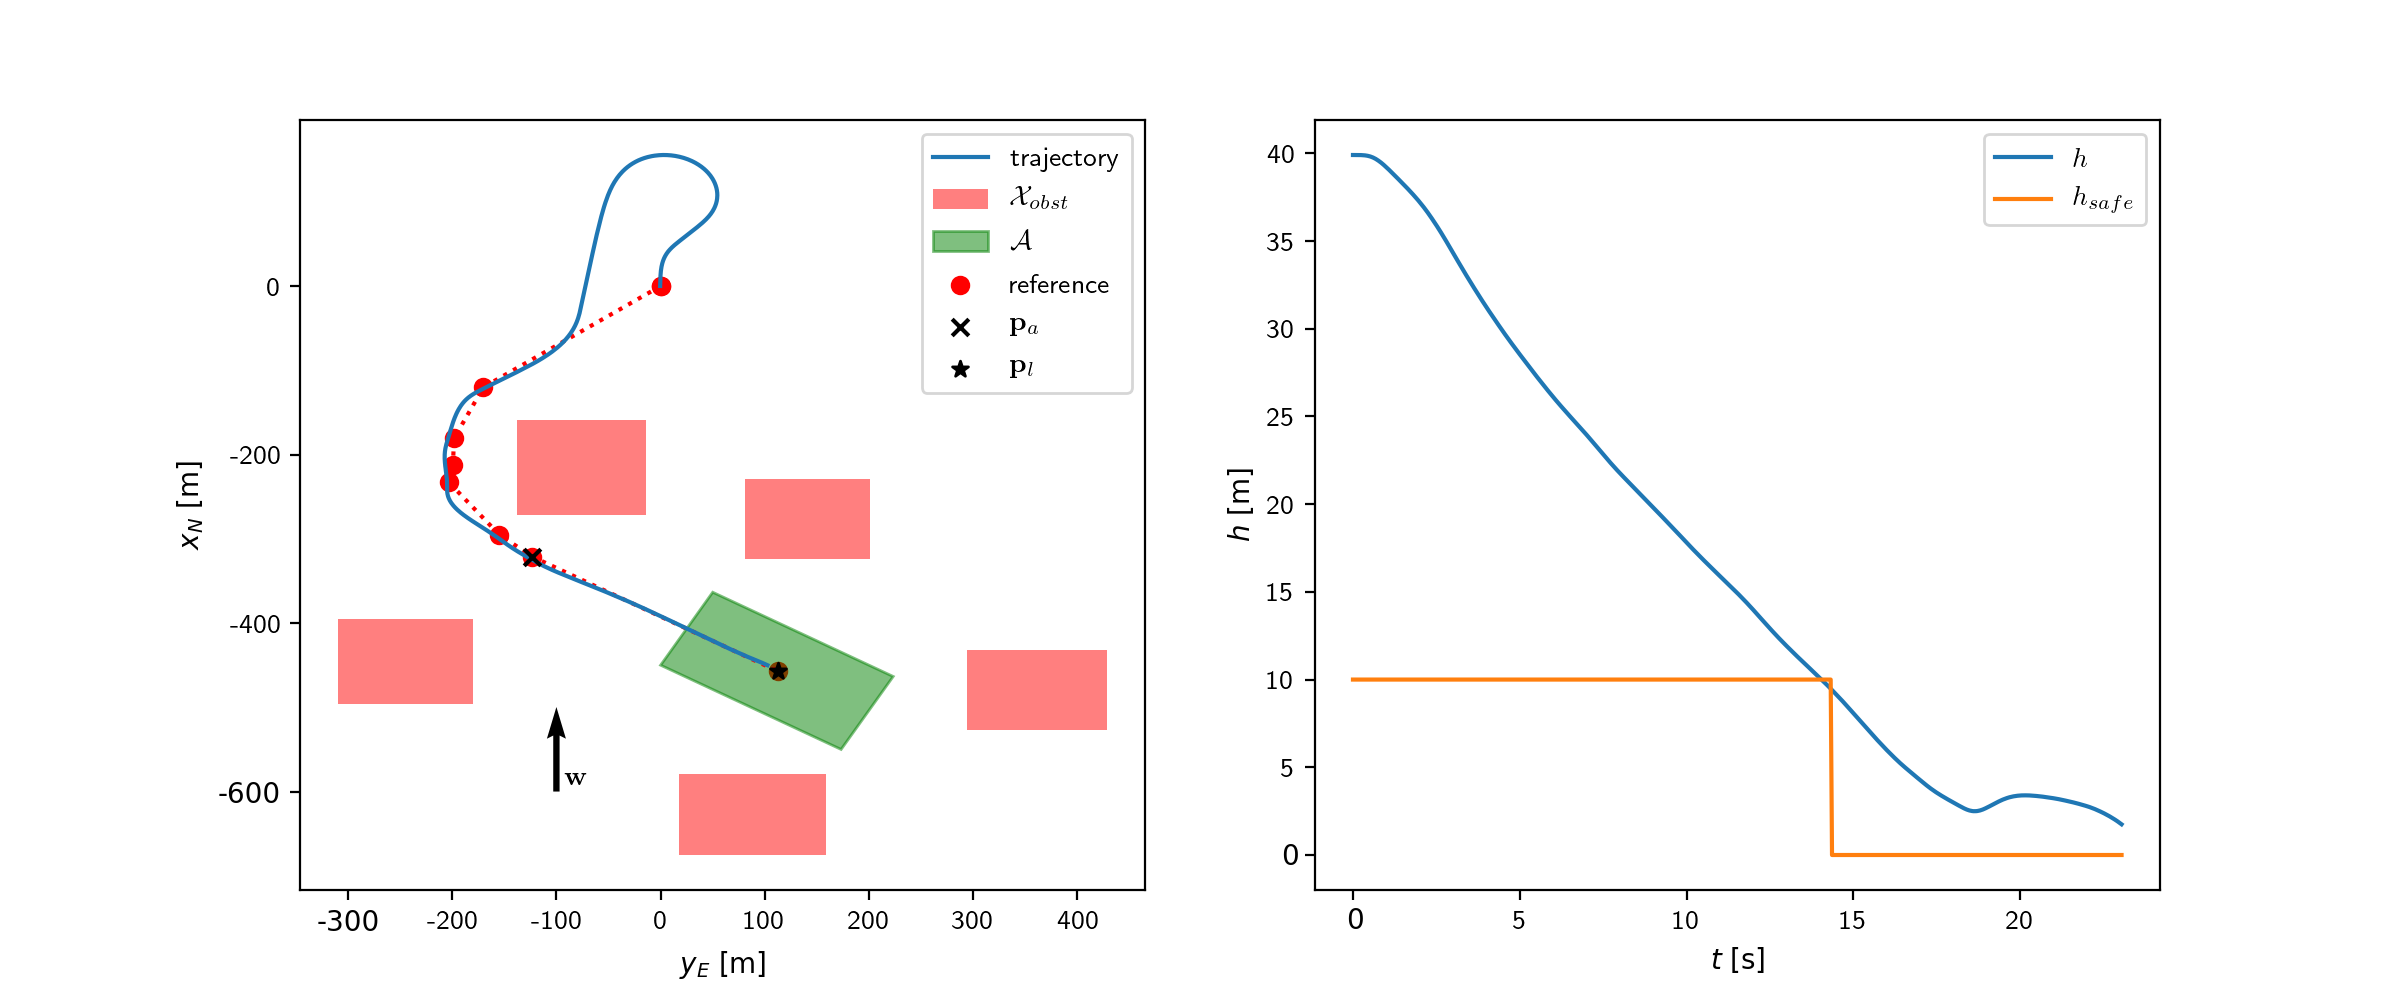
\includegraphics[width=1.3\textwidth]{sol_0}
    \caption{Landing sequence and altitude profile for $\winddir=0\degree$}
    \label{fig:sim_sol_0}
\end{figure}

\begin{figure}[H]
    \hspace{-0.15\textwidth}
    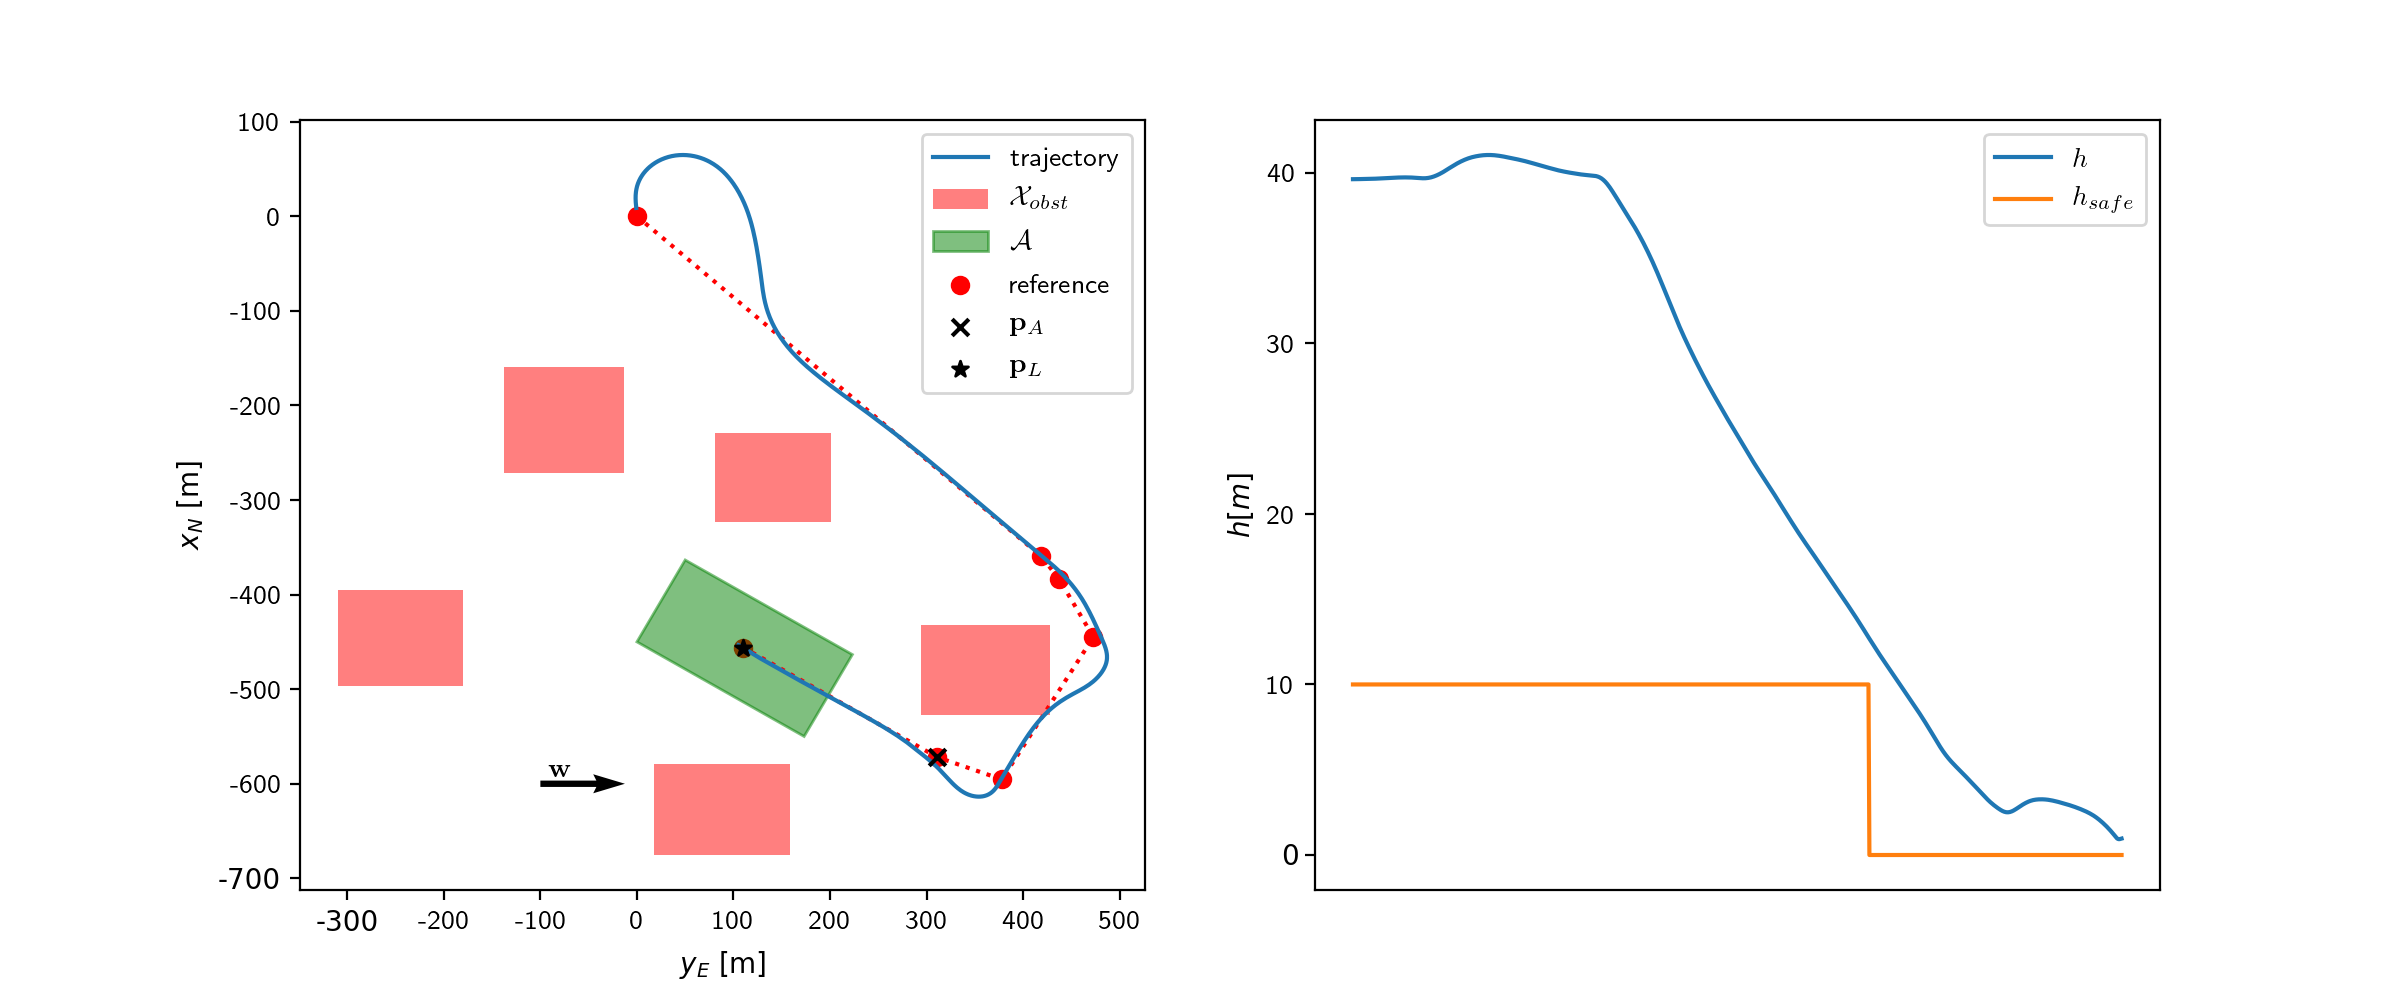
\includegraphics[width=1.3\textwidth]{sol_90}
    \caption{Landing sequence and altitude profile for $\winddir=90\degree$}
\end{figure}

\begin{figure}[H]
    \hspace{-0.15\textwidth}
    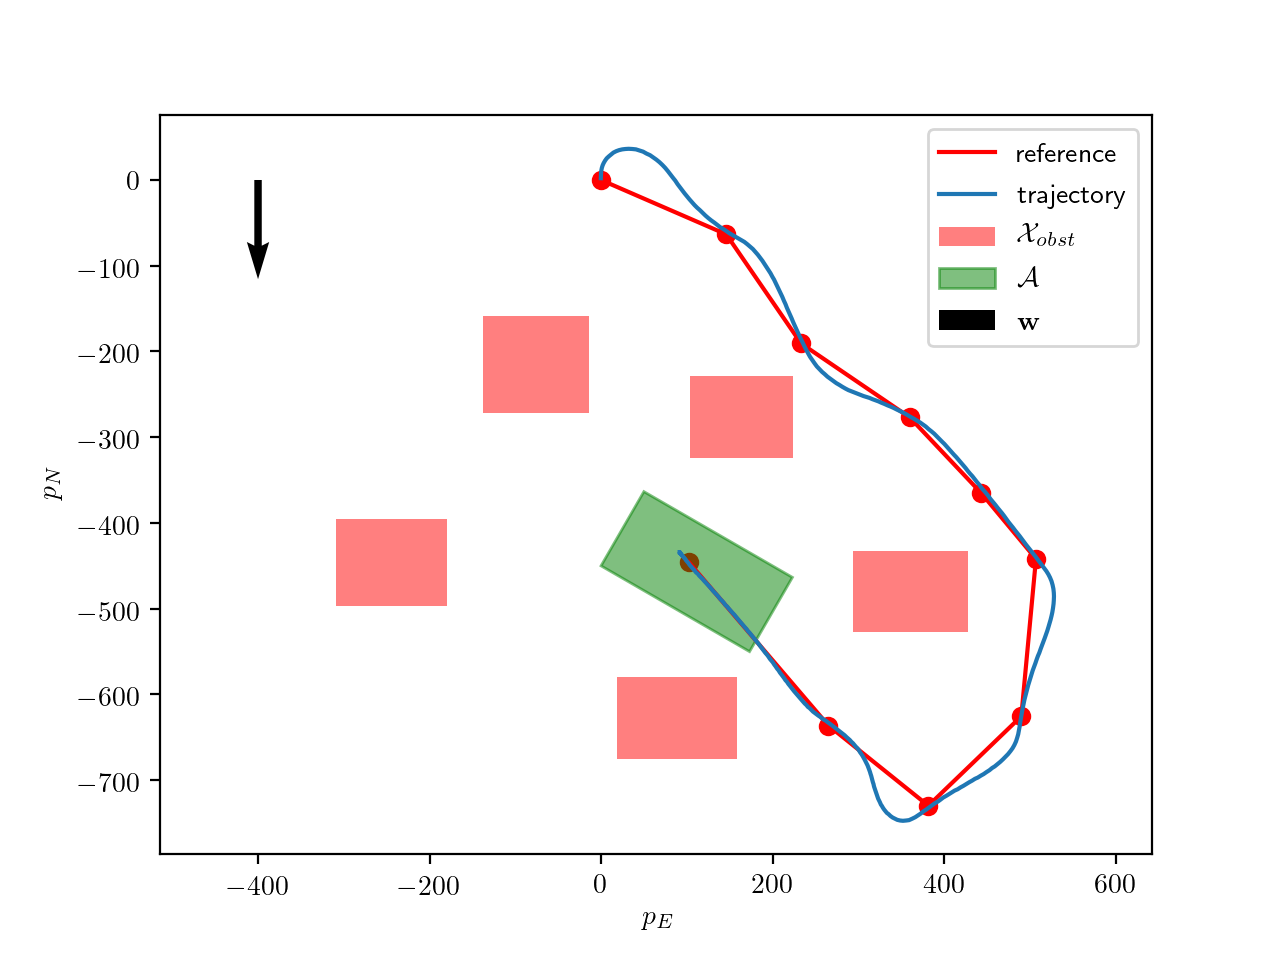
\includegraphics[width=1.3\textwidth]{sol_180}
    \caption{Landing sequence and altitude profile for $\winddir=180\degree$}
\end{figure}

\begin{figure}[H]
    \hspace{-0.15\textwidth}
    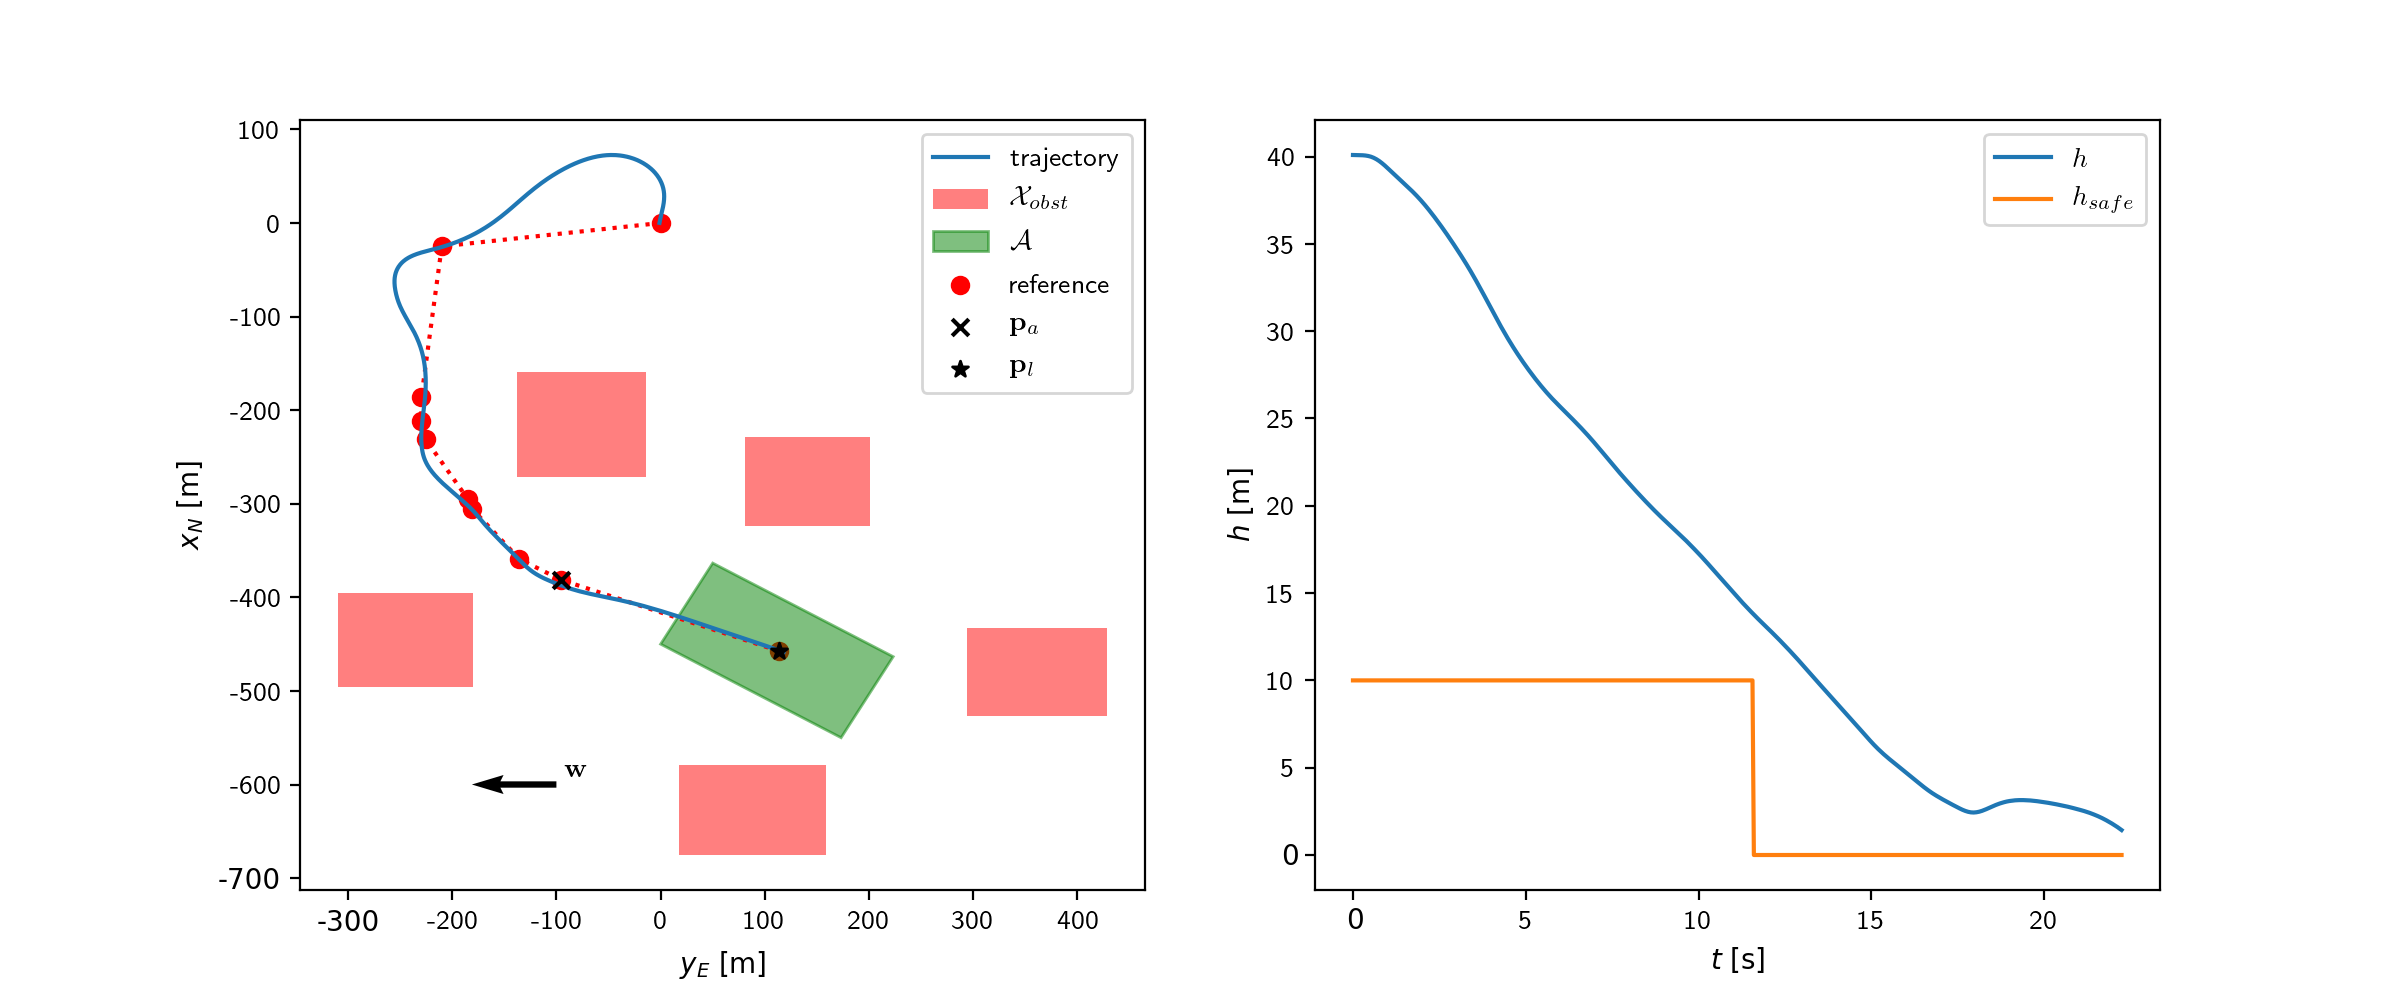
\includegraphics[width=1.3\textwidth]{sol_270}
    \caption{Landing sequence and altitude profile for $\winddir=270\degree$}
    \label{fig:sim_sol_270}
\end{figure}

\subsection{Discussion}
The results from simulation experiments indicate that the method successfully generates feasible landing 
sequences in different wind conditions. The distance between the planned and actual landing point is negligible relative to the total distance of the landing sequence.
The relative magnitude of the error in entry altitude is larger, but also seems quite constant, at least in the simulated evaluations summarized in Table \ref{tab:opt_land_param}. 
This implies that the error could be mitigated by estimating this offset and adding it to the desired $h_{\text{safe}}$. The error could also be mitigated by scaling the second term in the objective of 
Equation \eqref{eq:opt_problem_land} with some constant $\lambda_h>1$. The landing sequence generation is also quite fast, and a solution is found in well below 1 second in most cases.


\section{Real flight experiments}
In this section, setup and results of real flight experiments are presented.
\subsection{Experimental setup}
The \ac{uav} used during real flight experiments is shown in Figure \ref{fig:parrot}. This platform is based on a Parrot Disco airframe \cite{parrot}, 
which was modified to use the PixRacer autopilot \cite{pixracer} with Arduplane flight control software \cite{arduplane}. The \ac{uav} is also equipped with a 
Raspberry Pi 3B+ companion computer on which the landing system was deployed. The companion computer communicates with an external command and control interface using 
a 4G-LTE modem. The internal components of the \ac{uav} are shown in Figure \ref{fig:payload}, labeled as follows:
\begin{enumerate}
    \item Pitot tube sensor.
    \item 4G-LTE modem.
    \item Raspberry Pi companion computer.
    \item PixRacer autopilot.
    \item GPS receiver.
\end{enumerate}

\begin{figure}[H]
    \centering
    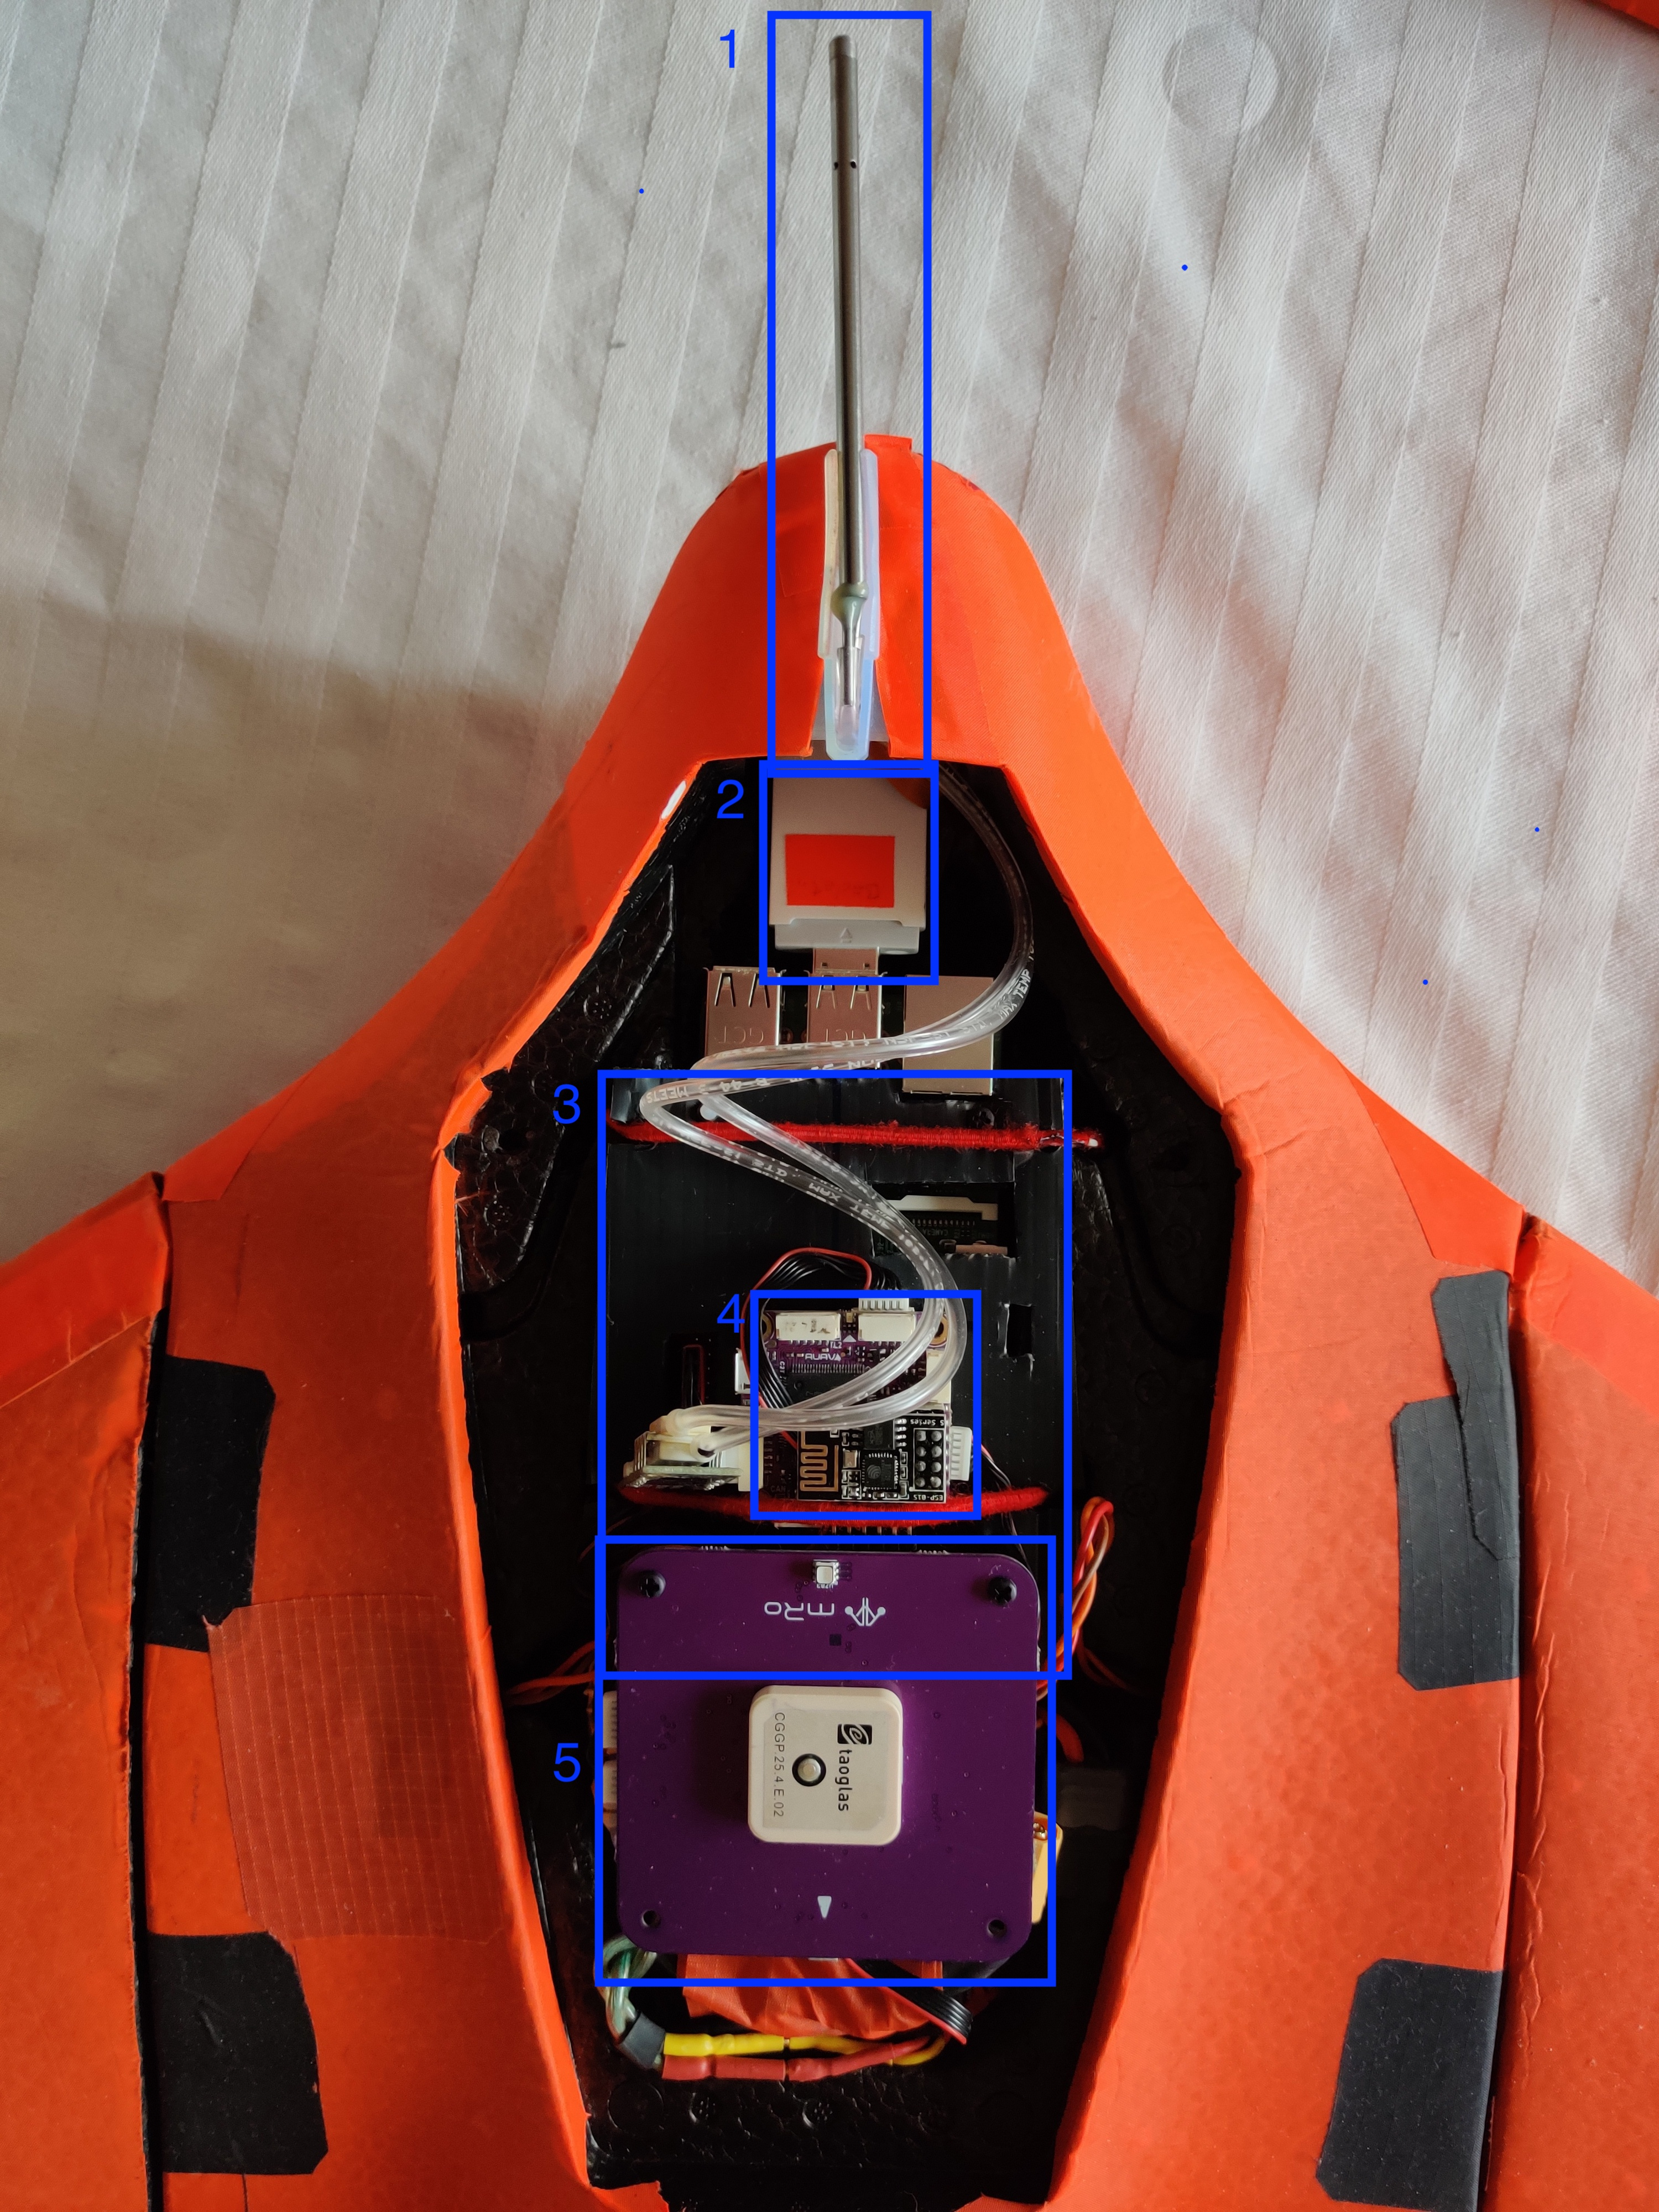
\includegraphics[width=.75\textwidth]{payload}
    \caption{Internal components of the \ac{uav} platform.}
    \label{fig:payload}
\end{figure}

\begin{figure}
    \begin{center}
        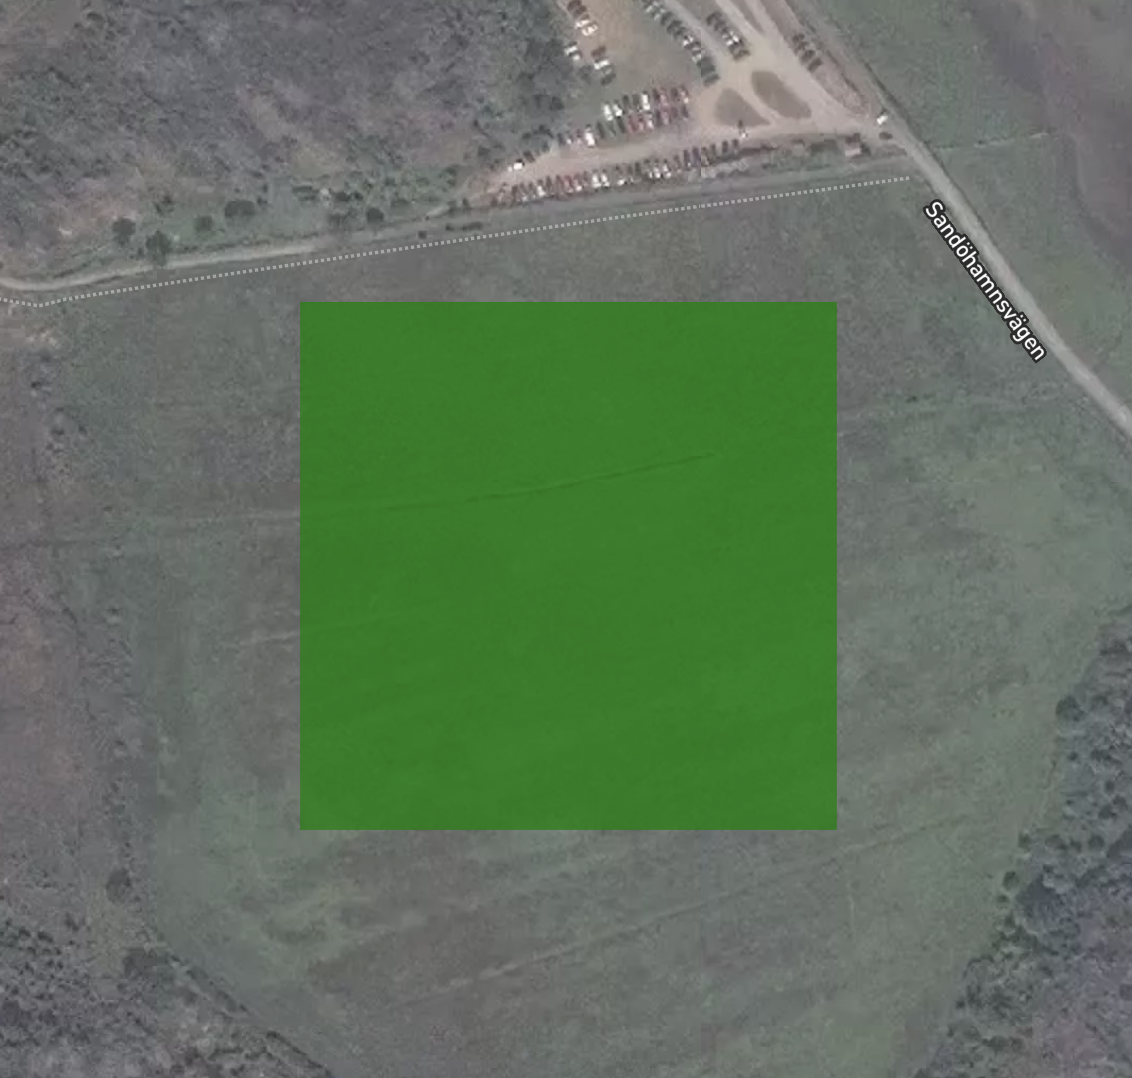
\includegraphics[width=.6\linewidth]{landing_map}
    \end{center}
    \caption{Landing area used for real flight experiments. Map data from Open Streetmap.}
    \label{fig:real_land_area}
\end{figure}

Experiments were conducted in an area near Longitude 11.929 and Latitude 54.486 south of Gothenburg, Sweden which is shown in Figure \ref{fig:real_land_area}.
The following procedure was followed during the experiments:
\begin{enumerate}
    \item Launch and takeoff with the \ac{uav}.
    \item Put the \ac{uav} in circular movement around a pre-defined coordinate $\vec{p}_{\text{loiter}}$, until the wind measurement has converged to an almost constant value.
    \item Compute $\vec{p}_a$ and $\vec{p}_l$ using the estimated wind direction and speed.
    \item Compute a waypoint mission from $x_0$ to $x_g=(x_{N,a},y_{E,a},\psi_l^*)$ with $x_0$ determined as described below.
    \item Send the computed mission to the autopilot and initiate mission execution.
\end{enumerate}

\subsection{Determining the starting state}
Since the motion planning algorithm assumes that the initial state of the \ac{uav} is exactly equal to the initial state used during planning, it is important 
that any positioning or heading errors are made as small as possible. This implies that $\vec{p}_{\text{loiter}}$ cannot be used directly as $x_0$ since the \ac{uav} circles around it, and thus 
the position and heading depends on when the landing sequence computation is initiated as well as the computation time which is uncertain.
Hence the starting state was determined by defining
\begin{equation}
    \vec{p}_{\pm90\degree} = \vec{p}_{\text{loiter}} + D\hat{r}_{\pm90\degree}
\end{equation}
where $\hat{r}_{\pm90\degree}$ is a unit vector pointing in the direction $\winddir\pm90\degree$ and $D$ was set to 100 m. The starting state was then set to
\begin{equation}
    x_0 = (x_{N,\pm90\degree},y_{E,\pm90\degree},\winddir\pm90\degree)
\end{equation}
depending on which of those points was closest to $\vec{p}_a$. This gives the \ac{uav} enough distance to reach the starting state exactly independent 
of where in the circular movement around $\vec{p}_{\text{loiter}}$ it is located when the mission is started.


\subsection{Results}
The trajectory and altitude profile of the \ac{uav} during a real landing is shown in Figure \ref{fig:real_land}. The estimated trajectory which was produced by the planner by forward simulation of the closed loop system is also shown. 
The reported wind speed and direction from the Swedish Meteorological and Hydrological Institute, SMHI at the time of the experiment was 
$\windspd=5$ m/s with gusts of 10 m/s, and $\winddir\approx120\degree$. The filtered estimates of both $\windspd$ and $\winddir$ during the flight are shown in Figure \ref{fig:real_wind}. The mean values used during planning were 
$\windspd=8.2$ m/s and $\winddir=118.8\degree$. The distance between planned and actual landing points in this experiment was $|R_l-R_l^*|=31$ m. 

 \begin{figure}
    \hspace{-0.15\textwidth}
    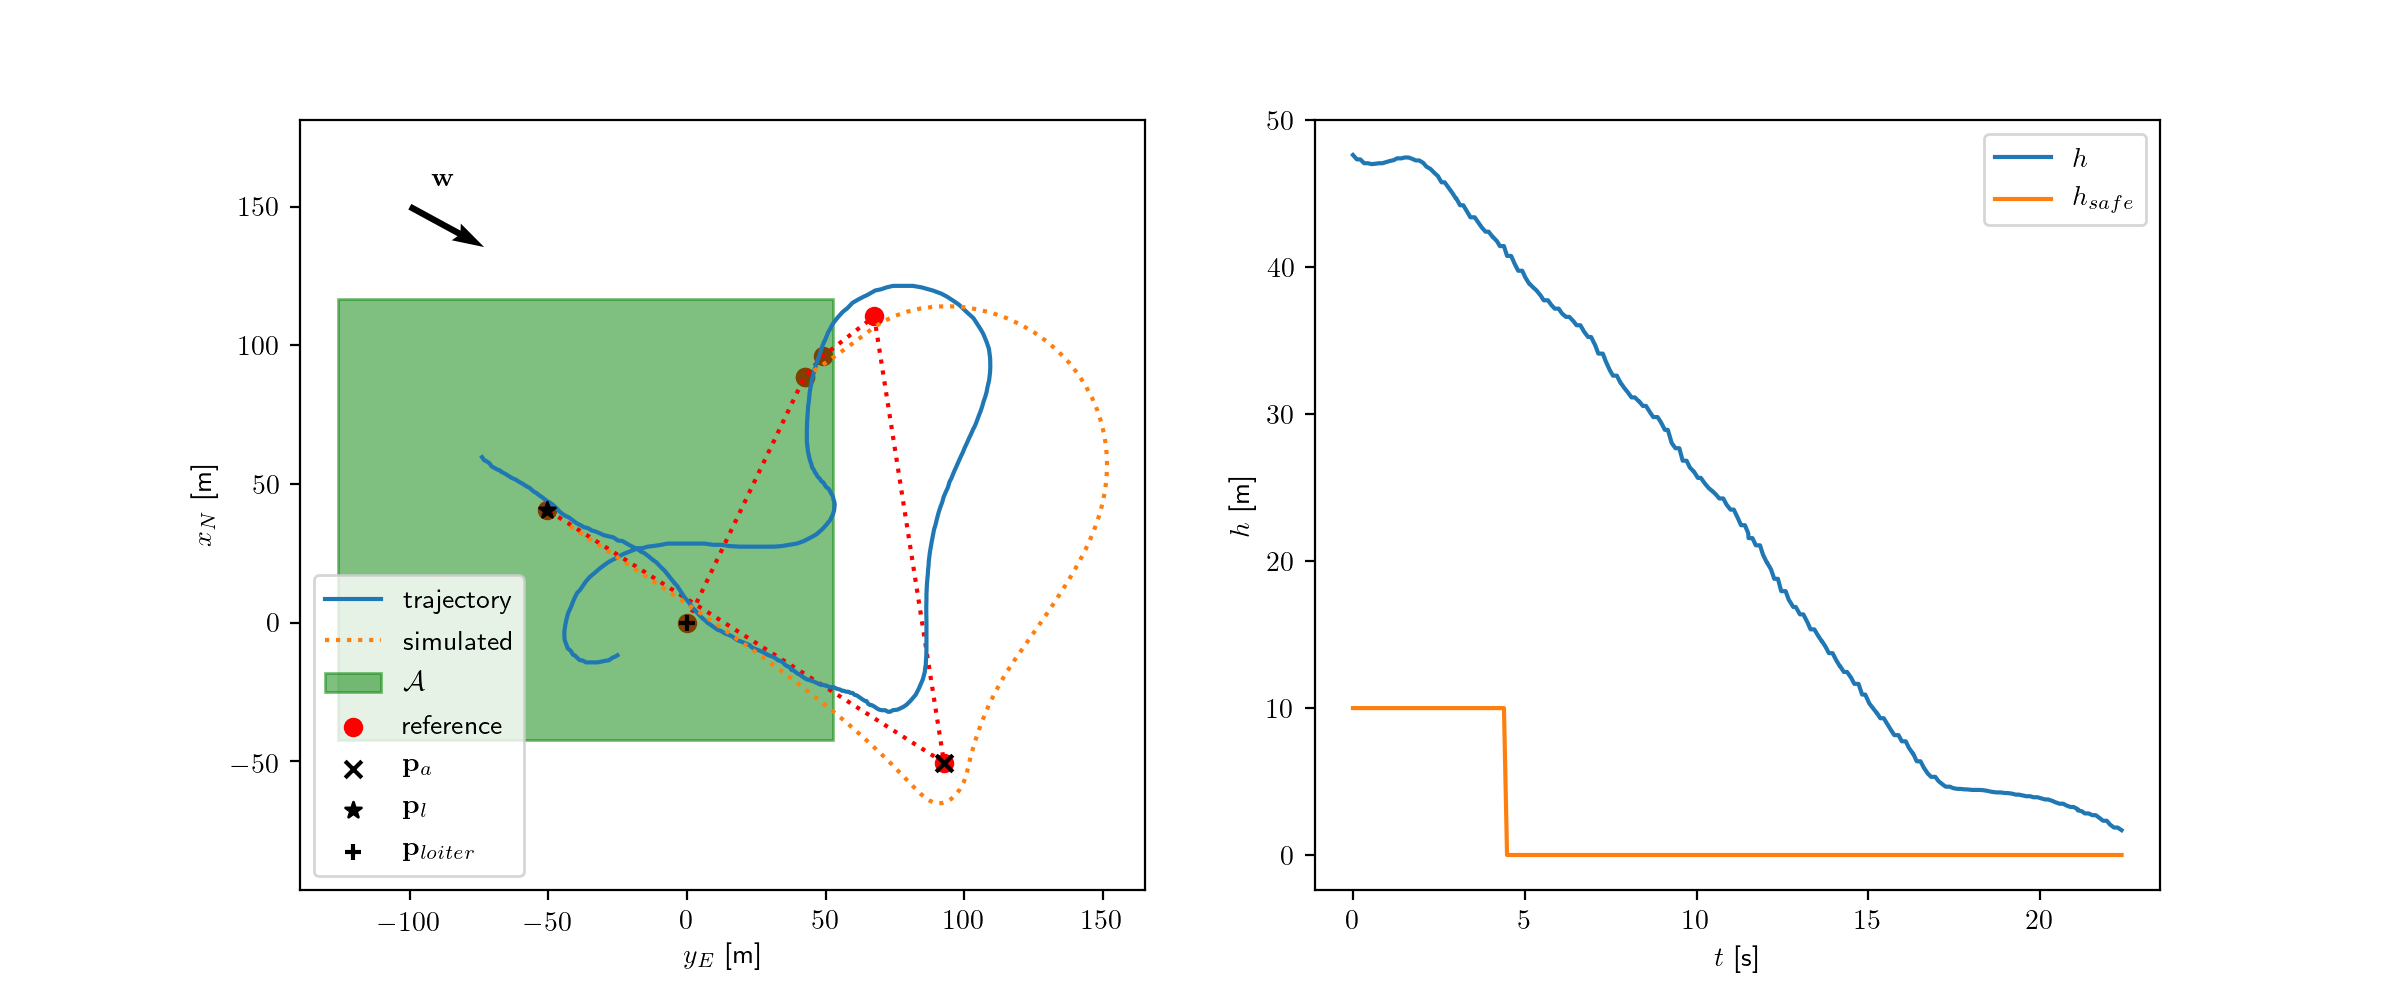
\includegraphics[width=1.3\textwidth]{real_flight}
     \caption{Trajectory and altitude profile of the real uav during execution of a landing sequence. The first waypoint is the point $\vec{p}_{\text{loiter}}$ which the \ac{uav} circles around while the landing sequence is calculated. 
     To compensate for the unpredictable initial heading when the landing sequence is initiated, the initial state is placed at a fixed distance from $\vec{p}_{\text{loiter}}$ in a direction perpendicular to the estimated $\winddir$.}
     \label{fig:real_land}
 \end{figure}

 \begin{figure}
    \hspace{-0.15\textwidth}
    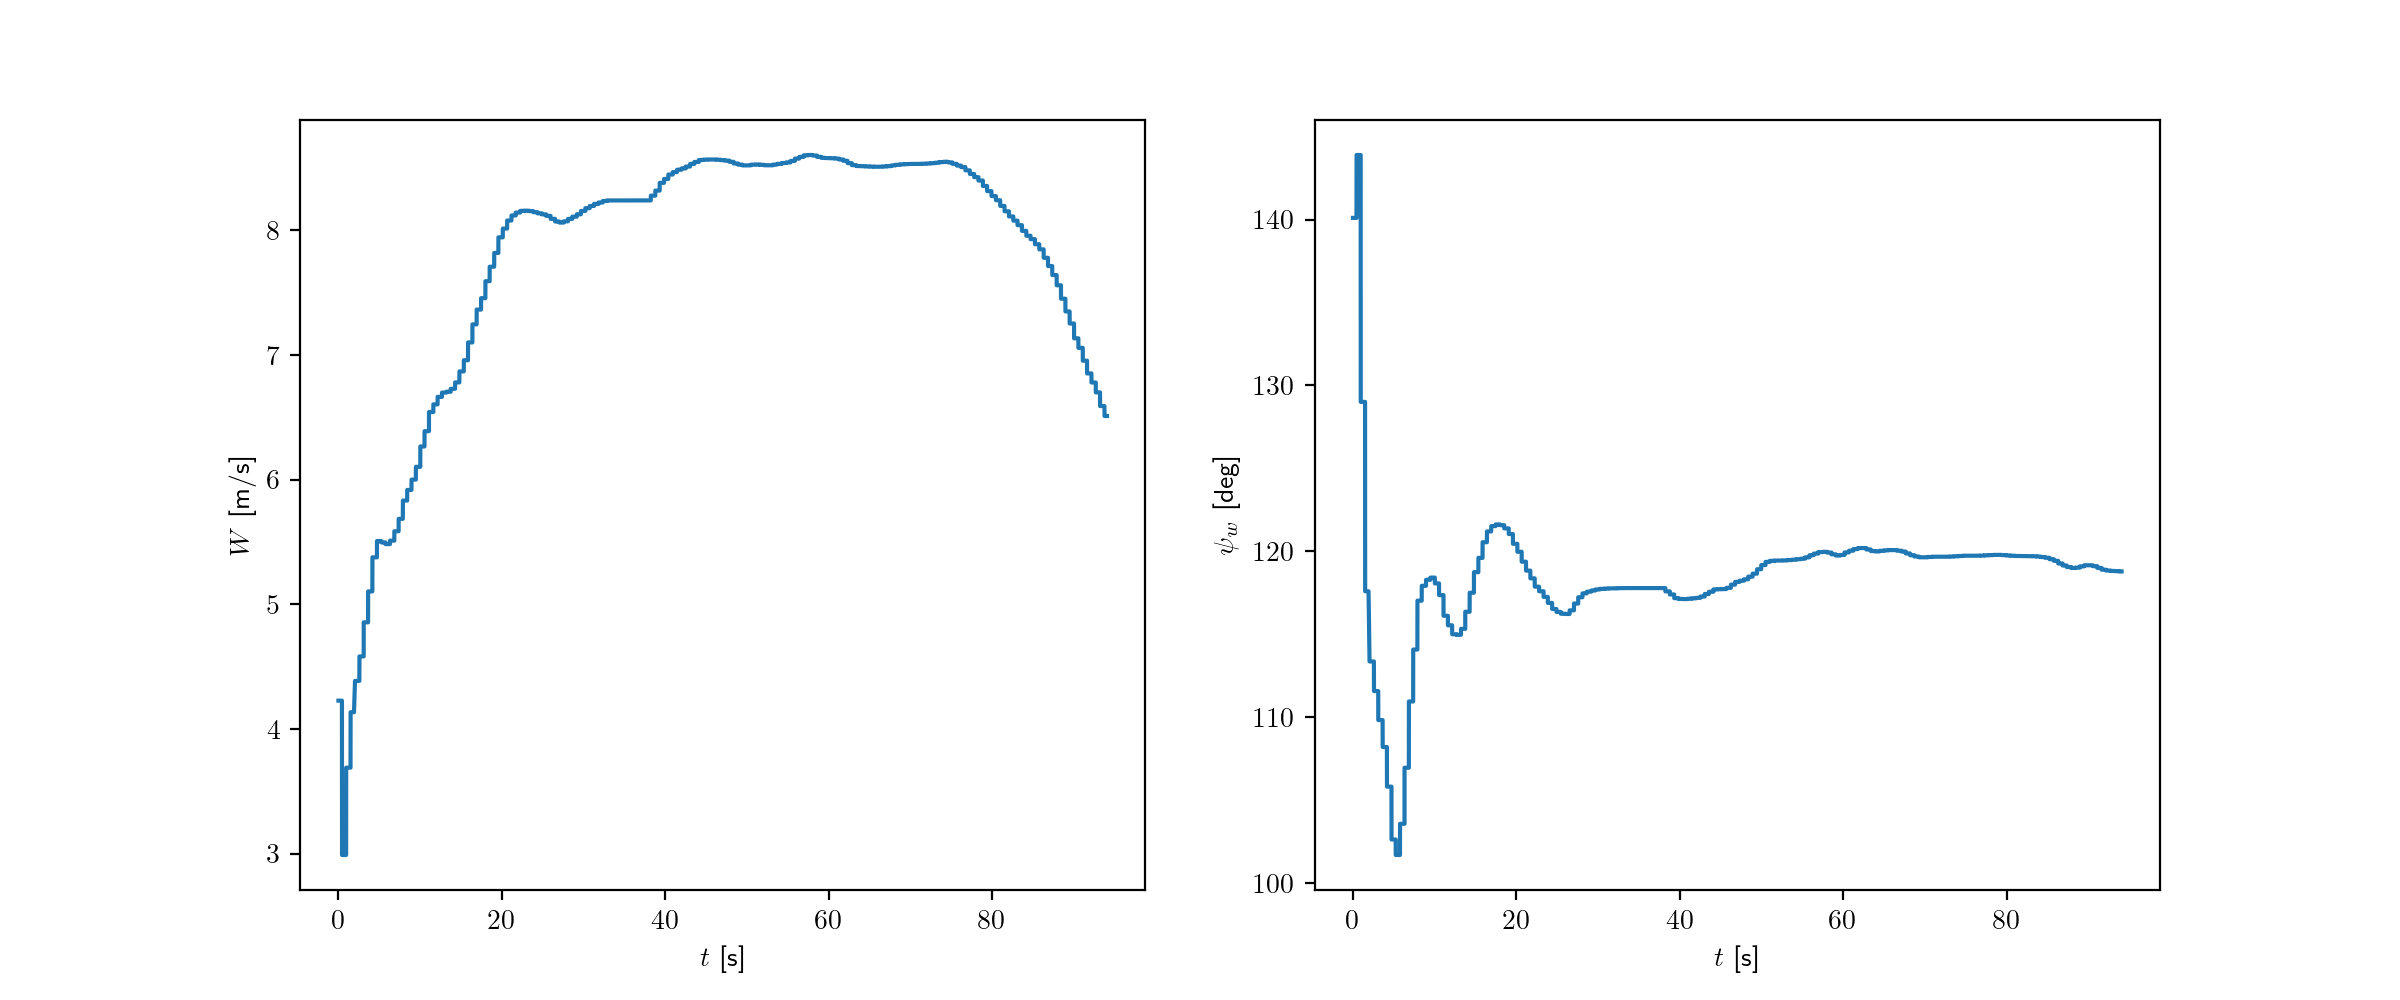
\includegraphics[width=1.3\textwidth]{real_wind}
    \caption{Filtered estimates of $\windspd$ and $\winddir$ during real flight experiment. Both plots show values from the entire duration of the flight, \ie\, from the moment the \ac{uav} takes of until it lands on the ground again.}
    \label{fig:real_wind}
 \end{figure}

 \subsection{Discussion}
In the real landing experiment, the distance between planned touchdown point and the actual was significantly larger than 
in the simulations. One reason for this, as can be seen in Figure \ref{fig:real_land}, is an inconsistency in value of the parameter $R_{\text{wp}}$, which determines how close the \ac{uav} should be to a target waypoint in 
order for it to be considered reached, between the planner and the autopilot. Since the expected wind speed was 5 m/s, the inputs used during planning were calculated for $\windspd\in[3.75, 6.25]$. The actual windspeed, however, turned out to be significantly higher. 
As such, using inputs computed for wind-speeds in an interval centered around $\bar{W}\approx8$ m/s would probably increase the accuracy further. It can also be noted that there is an overshoot in the trajectory following controller during the first 
straight-path segment. This might be caused by an unexpected wind gust, but such overshoots could probably be reduced by increasing the look-ahead distance $L_1$ of the controller.

To ensure a safe landing, the selected landing area for this experiment was quite large and thus the constraint on safe entry altitude was negligible. 
Nevertheless, the results are promising, and the method should be evaluated further by performing additional real flight experiments in more challenging scenarios.
\chapter{Conclusions}\label{cha:discussion}
\section{Results}
In this work, a novel method to automatically generate landing sequences for fixed-wing \acp{uav} is proposed. 
The method automatically handles many of the challenging aspects when specifying such a sequence manually, \eg\ taking the current 
direction and speed of the wind into account.

The method consists of two main components, the \textit{landing sequence calculation} and \textit{motion planner}. Both these components mainly rely on optimization-based methods. 
To calculate the parameters determining the landing sequence, \ie\ when the \ac{uav} descends to the ground, a non-linear optimization problem is 
formulated and solved numerically. The motion planner uses a set of precomputed waypoints together with sampling-based planning techniques to determine a plan which is feasible given the 
\ac{uav} model and current wind conditions. To create the set of waypoints, an optimization problem is solved using derivative-free optimization.

The proposed method is quite general and could be implemented on any fixed-wing \ac{uav} which uses the trajectory controller described in Section \ref{sec:traj_controller}. 
It would also be easy to extend it to support another controller, as the only requirement to create the input set $\inputs$ is that the closed-loop model of the system is written on the same form as 
Equation \eqref{eq:closed_loop}.

\section{Limitations of the method}
Constraining the control reference to consist of waypoints, \ie\ straight line-seg\-ments, limits the system from using more complex trajectories like the ones used in \cite{emergency_landing}. It also introduces some issues mentioned in Chapter \ref{cha:results}. 
However, most popular autopilots, such as Ardupilot, use this formulation \cite{arduplane}. 

Sampling methods contain inherent limitations, such as the 
quality of the solution depending on the sampling resolution. In many cases, such as when generating a \ac{hlut}, there is also a tradeoff between resolution and storage capacity. In the case of a 2-dimensional \ac{hlut} as in this thesis, the \ac{hlut} size scales quadratically with the sampling resolution used. 
However, calculating analytical solutions in realtime is often infeasible due to high computational costs.

A large limitation of the landing area definition in Chapter \ref{cha:landing} is the assumption that the terrain elevation is constant inside the landing area $\landing$. In 
most real-world cases, such as landing in a slope, the terrain elevation varies. Including this factor in the landing sequence generation would enable landings in a much wider class of scenarios.

The assumption that the wind is constant simplifies many parts of calculating the landing sequence, but such an approximation also introduces limitations in the performance of the method. As can be seen in Figure \ref{fig:real_wind}, the windspeed $\windspd$ is quite constant while the \ac{uav} is flying at a constant altitude. However, there is a clear altitude dependency in the 
wind-speed estimate, which is visible both during the takeoff and landing portions of the flight. It is therefore likely that including this altitude dependency, especially in the calculation of the final descent parameters $\vec{p}_a$ and $\vec{p}_l$ could increase the precision of the landing.

\section{Future work}
The landing sequence method depends on many different parameters, both air\-frame-specific such as $\dot{\psi}_{\text{max}}$ and general such as discretization step-sizes and wind speeds used for input generation.
The goal of this thesis was mainly to evaluate the feasibility of the proposed method. Hence, most of those parameters were set to "good-enough" values which proved to be feasible but are not necessarily optimal. 
A possible future work consists of tuning these parameters for the currently used \ac{uav} platform, which would require a number of real-world flight experiments in different wind conditions.
It would also be interesting to study methods to efficiently and automatically estimate optimal values of these parameters, especially those specific to the airframe.

As mentioned, an important future work is to include terrain elevation in the landing sequence generation. Another important area is to 
study how an additional system mounted on the \ac{uav} could automatically detect suitable landing areas, \eg\ using vision sensors and an elevation and obstacle database. 
This would be a step towards truly autonomous fixed-wing \acp{uav}, as the system would be able to perform a safe landing without any pilot input. It could also be used to perform 
emergency landings if the command and control link to the pilot is lost.


%\chapter{Resultat!}\label{cha:Research}
Det här är kapitlet där resultaten presenteras!!!!!!!!!!!.
asdasdasdasdasdadsads


\section{Ditten}\label{sec:research:history}
%
Liksom \citep{Duck:2005} har vi kommit fram till att glass smakar bäst på sommaren.

\marginpar{Kommer att tänka på en liten anekdot\ldots}

\Warning[TODO]{Ta bort den löjliga anekdoten!}

När vi nu går in på hur glass smakar vid olika tidpunkter under dagen hänvisar vi till \figureref{fig:times}, och speciellt till \figureref{fig:times:early}.  Jämför sedan med \figureref{fig:times2} för att se hur det kan bli när man äter glass vid okontrollerade tidpunkter.

Veselić, Krešimir (Veseli\'{c}, Kre\v{s}imir) skrev en gång en artikel med titeln \emph{Bounds for exponentially stable semigroups}.

\begin{figure}[tbp]
  \centering
  \subfloat[Alldeles för tidigt.][\label{fig:times:very-early}Det här är väl tidigt — din glass hinner smälta innan ditt sällskap dyker upp.]{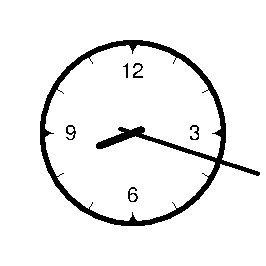
\includegraphics[page=1]{clocks}}
  \qquad
  \subfloat[Med marginal.][\label{fig:times:early}Kiosken stänger snart, men inte nu — perfekt!]{\includegraphics[page=2]{clocks}}
  \\
  \subfloat[I grevens tid.][\label{fig:times:on-time}Precis i tid — du får in ett finger i luckan just när kiosken ska stänga.  Han som jobbar blir sur, och det blir smolk i bägaren.]{\includegraphics[page=3]{clocks}}
  \qquad
  \subfloat[Försent.][\label{fig:times:late}Du är sen — kiosken är stängd.]{\includegraphics[page=4]{clocks}}
  \caption{\label{fig:times}%
    Illustration av \emph{subfloats}.  Den så kallade \emph{bounding box}en visas i \protect\subref{fig:times:late}.  Lägg märke till att bounding boxen har satts så att alla bilder har samma storlek, med enhetlig placering av själva innehållet i förhållande till bounding boxen.  Antag att du ska träffa en kompis för att äta glass just när kiosken stänger för dagen vid 08:30.  När dyker du upp?}
\end{figure}

\begin{figure}[tbp]
  \centering
  \subfloat[][\label{fig:times2:very-early}]{\includegraphics[page=5]{clocks}}
  \qquad
  \subfloat[][\label{fig:times2:early}]{\includegraphics[page=6]{clocks}}
  \\
  \subfloat[][\label{fig:times2:on-time}]{\includegraphics[page=7]{clocks}}
  \qquad
  \subfloat[][\label{fig:times2:late}]{\includegraphics[page=8]{clocks}}
  \caption{\label{fig:times2}%
    En andra illustration av \emph{subfloats}.  Den här gången har bounding boxen gjorts så liten som möjligt runt själva innehållet.  Resultatet är stökiga placeringar på sidan.  Samma sak kan hända med vanliga fyrkantiga figurer när man har text som spretar ut åt lite olika håll från själva rutan med kurvor i.}
\end{figure}

\section{Framtiden}

Sen när glassen är uppäten är det bara till att sätta igång och skriva på exjobbet igen!


\begin{chapter-appendix}

\section{Ett par långa bevis}
%
Det här är en appendix-del av det aktuella kapitlet.

\end{chapter-appendix}

%\chapter{Avslutande kommentarer}\label{cha:conclusions}
%
Sätt av ett kort kapitel sist i rapporten till att avrunda och föreslå rikningar för framtida utveckling av arbetet.


%\part*{Appendix}
\appendix
%\chapter{Trista saker}\label{cha:boring}
Långa beräkningar brukar bli rätt trista\dots

Detta är ett appendix-kapitel.  Jämför med appendixet i \chapterref{cha:Research}.

\section{Bädda sängen}

Den här beräkingen är så trista att vi kallar den \emph{att bädda sängen}.

\section{Diska}

Den här beräkingen är så trista att vi kallar den \emph{att diska}.

%\chapter{\rtthesis documentation and \LaTeX{} tips}\label{cha:rtthesis}

This document is not only an example that you can use to get started with the \rtthesis class, it also contains written instructions for how to use the class, and some general tips on how to use \LaTeX{} to produce a beautiful thesis.  As we do so in this chapter, we also get the opportunity to look at some theorem-like environments, which you can alter the look of by changing the options given to the \rtthesis class.

\section{Basic setup}\label{sec:basic-setup}
%
You must decide on an input encoding from start, and select the corresponding class option from \tableref{tab:inputenc} on \pagepageref{tab:inputenc}.  You must also tell \rtthesis whether you intend to use part sectioning or not, see \tableref{tab:part-options}.  There are many more class options, but they will be mentioned below where there is room for a more detailed discussion for the corresponding features.

Information about the thesis, which is needed to produce the thesis itself as well as the thesis cover and the “spikblad”, is passed to \rtthesis using the command \texcommand{setupThesis}.  The command is called in the following way, where the most common key-value pairs are listed in \tableref{tab:setupThesis} (the remaining key-value pairs concern master's theses, see \sectionref{sec:msc})):

\begin{minipage}{1.0\linewidth}
  \verbatimsize
\begin{verbatim}
\setupThesis{
  key1=value1,
  key2=value2,
  ...
}
\end{verbatim}
\end{minipage}

If a PhD thesis has an interesting illustration on the cover, it is customary to provide a caption for the illustration.  The caption will be printed on the back of the title page, and is set up by redefining the command \texcommand{rtcoverinfo}.  For instance, it may look like this:

\begin{minipage}{1.0\linewidth}
  \verbatimsize
\begin{verbatim}
\renewcommand{\rtcoverinfo}{\textbf{Cover illustration:}  Block
diagram showing the structure of the control scheme proposed in
\chapterref{cha:cool-control}}
\end{verbatim}
\end{minipage}


\begin{table}[tbp]
  \centering
  \caption{\label{tab:part-options}%
    Class options that inform \rtthesis whether part sectioning will be used or not.}

  \begin{tabular}{l p{0.5\linewidth}}
    \toprule%
    \textbf{Class option} & \textbf{Meaning} \\
    \otoprule%
    \classoption{parts} & Prepare for \texcommand{part} as the topmost sectioning command.\\
    \classoption{noparts} & Prepare for \texcommand{chapter} as the topmost sectioning command.\\
    \bottomrule%
  \end{tabular}
\end{table}

\begin{table}[tbp]
  \centering
  \caption{\label{tab:setupThesis}%
    Key-value pairs recognized by \texcommand{setupThesis}.  Note that values that include white space are surrounded by braces.}

  \begin{tabular}{>{\ttfamily}r !{\texttt{=}} >{\ttfamily}l p{0.5\linewidth}}
    \toprule%
    \textbf{Key} & \textbf{Example value} & \textbf{Comment} \\
    \otoprule%
    author & \{My Name\} & \\
    title & \{Thesis title\} & \\
    subtitle & \{Good stuff\} & Optional. \\
    city & Norrköping & Default: \emph{Linköping} \\
    year & 2010 & \\
    isbn & isbn-isbn-isbn-isbn & \\
    type & phd & Must be either \emph{phd}, \emph{lic}, or \emph{msc}. \\
    thesisNo & 9999 & Number in series (the series is determined by the choice of thesis type). \\
    localID & 11 & Only used for licentiate's theses.  It is the last part of the local identifier \emph{\mbox{LIU-TEK-LIC-2010:11}} in this case.\\
    username & isyusername & Used to generate the author's email address. \\
    dedication & \{To my parents!\} & \\
    \bottomrule%
  \end{tabular}
\end{table}

\section{Page layout and related options}\label{sec:page-layout}
%
Theses are restricted to the S5 paper size.  How the S5 page is organized is up to you, but \rtthesis only allows you to choose from two predefined layouts, and only one of them is recommended.  To get your own layout you should make a copy of \textfilename{rtthesis.cls} and modify the code for one of the existing class options for layout.  The class options for page layout are given in \tableref{tab:page-layout}.

At the time of writing, the printers used by LiU-Tryck print on A4 paper (physical size), which is then cropped to S5 (logical size).  Similarly, when you print draft versions of your thesis on your office printer, it is very likely that the used physical paper size will be A4.  Hence, it makes sense to let \rtthesis control how the S5 logical page is placed on the A4 physical paper.  In this case, \rtthesis will produce a \textsc{pdf} with pages in the A4 format, with content restricted to the S5 format.  On the other hand, when you produce a \textsc{pdf} that is meant to be read on a computer screen, the page size should be exactly S5.  When targeting the A4 physical format, it is possible to get crop marks for the S5 box, and to put some information about each page outside the S5 box.  The related class options are given in \tableref{tab:page-layout}.

To ensure that you really get the page layout you think when you send your thesis file to the printer's, the best option \emph{should} be to use the \classoption{crop} option.  However, they will tell you differently, since they think it's \emph{their} job to position the logical page on A4 and add crop marks.  Unfortunately, there is a lot of manual work in the process, so there is a (substantial?!) risk that the content of your pages will be shifted with respect to the S5 box of your layout\ldots

\begin{table}[tbp]
  \centering
  \caption{\label{tab:page-layout}%
    Class options related to page layout.  The most important one to remember is \classoption{crop} (since  \classoption{S5} and \classoption{pdf} are default).}

  \begin{tabular}{l p{0.5\linewidth}}
    \toprule%
    \textbf{Class option} & \textbf{Meaning} \\
    \otoprule%
    \classoption{S5} & Recommended layout.  Margin paragraphs are tiny (see \sectionref{sec:research:history} for examples), and should only be used for comments that will be removed in the final version of the thesis.  Default.\\
    \classoption{S5MP} & Layout to use if you are serious about margin paragraphs.  Not recommended, since the S5 format is too narrow to really fit margin paragraphs of reasonable width. \\
    \classoption{nailing} & Layout for the “spikblad”.  Not for theses! \\
    \midrule%
    \classoption{pdf} & Produce pages in the S5 format.  Default.\\
    \classoption{onA4} & Logical S5 page on a \textsc{pdf} page of size A4.\\
    \classoption{info} & Write information about each page above the logical S5 page.\\
    \classoption{crop} & Same as \classoption{onA4} with \classoption{info} and crop marks.\\
    \classoption{noInfo} & Turn off the effect of \classoption{info}.\\
    \classoption{draft} & Same as \classoption{onA4}, but pictures are blank and overfull \texttt{hbox}es stand out.\\
    \bottomrule%
  \end{tabular}
\end{table}

Although only weakly related to page layout, this section ends with a tip for how to change the size of the chapter numbers (some users find them much too big).  The font is controlled using the \styname{sectsty} package, and it follows that it can be redefined by, for instance,

\begin{minipage}{1.0\linewidth}
  \verbatimsize
\begin{verbatim}
\chapternumberfont{\fontsize{60mm}{63mm}\selectfont}
\end{verbatim}
\end{minipage}

\section{Front-matter environments}

There are environments defined for typical sections in the front-matter\footnote{The \emph{front-matter} is everything that goes in the beginning of the thesis, before the page numbered~\emph{1}.}.  The most important purpose of providing these environments is that they take care of the table of contents and the \textsc{pdf} bookmarks for you.  The environments are \envname{abstract}, \envname{preface}, \envname{acknowledgments}, and \envname{notation}.

The environment \envname{abstract} accepts the language used inside the environment as an optional argument (which defaults to \texttt{english}).  If the language is set to \texttt{swedish}, the title of the abstract will be \emph{Populärvetenskaplig sammanfattning}, in accordance with the Linköping University requirements on theses written in English.

Inside the \envname{notation} environment, you can put anything you like, and maybe the \envname{notationtabular} environment provided by \rtthesis suits your needs.  In order to define this environment, \rtthesis loads the two packages \styname{array} and \styname{booktabs}, and also defines the command \texcommand{otoprule} to mean the same as \texcommand{toprule}.  See \tableref{tab:notationtabular} regarding how to change the look of \envname{notationtabular}.

\begin{table}[tbp]
  \centering
  \caption{\label{tab:notationtabular}%
    Legal option values to the \envname{notation} environment.  The options control the look of the \envname{notationtabular} environments used inside the \envname{notation} environment.  The initial definition of \envname{notationtabular} is the same as that obtained by passing the option \classoption{new}.}

  \begin{tabular}{l p{0.5\linewidth}}
    \toprule%
    \textbf{Option} & \textbf{Meaning} \\
    \otoprule%
    \emph{emty} & Do not redefine \envname{notationtabular}.  Default.\\
    \classoption{old} & Make \envname{notationtabular} produce a plain \LaTeX{} table with double horizontal lines under the table headings, and a vertical line separating the two columns.\\
    \classoption{new} & Make \envname{notationtabular} produce a table according to the guidelines in \citet{Mori07Tables} using the \styname{booktabs} package.\\
    \bottomrule%
  \end{tabular}
\end{table}

There is a class option called \classoption{noextras}, which was intended to inhibit the effect of the \texcommand{maketitle} command, and redefine the front-matter environments to not produce any output.  However, the option is not working well at the moment.  On the other hand, as the time it takes to compile a thesis on a modern computer is very short, it is rather unclear why someone would like to use this feature anyway.


\section{Abbreviations}

Automatic control is a \LaTeX{}-friendly community.  This means that everything you produce is expected to look good.  We begin with a basic result.

\begin{theorem}\label{th:abbr-in-sc}
  Abbreviations, such as \abbrARMA, look best in small caps.

  \begin{proof}
    Just compare with “ARMA”.
  \end{proof}
\end{theorem}

However, it is important that the small caps match the sorrounding text, compare the statement in the theorem above with the following variation of it, in italics instead of slanted text:
\begin{quotation}
  \noindent\textit{Abbreviations, such as \abbrARMA\footnote{This will cause a \LaTeX{} warning.} or {\normalfont\textsc{arma}}, will stick out in a terrible way if you don't watch out!}
\end{quotation}
This is why the \rtthesis class uses slanted text rather than italics in theorems rather when slanted small caps are available.

Unfortunately, \rtthesis does currently not provide a way to make small caps look good in italics, which leads to the following corollary to \theoremref{th:abbr-in-sc}.

\begin{corollary}
  One has to make a choice between
  \begin{itemize}
  \item Beautiful abbreviations using small caps (instead of ordinary upper case).
  \item Pretty text typeset in italics (instead of slanted text).
  \end{itemize}
\end{corollary}

\section{Definitions}

Let us discuss another theorem-like environment while we have some examples of similar environments to compare with in the previous section.  That is, let us discuss the \envname{definition} environment (and the similar environments \envname{assumption} and \envname{remark}).  All the theorem-like environments are defined in a separate package, \styname{rtthesis-theorems}, so that they can be used with other document classes as well.  The definition below is an example of a definition with a title.

\begin{definition}[Definition]
  A \emph{definition} is a precise explanation of the meaning of a word or concept.  It may be tempting to include examples in a definition, but a good definition should not depend on examples as part of the definition.  However, examples are often useful to clarify a definition, and should appear near the definition.

  A short definition may require just a single paragraph, while a more complex definition may require a few paragraphs.  Some definitions will also make use of displayed math.
\end{definition}

One problem one has to consider if definitions are not restricted to just one paragraph, is how to show the reader where the definition ends.  In theorems, it is common to use italics or slanted text (for brevity, we will not mention italics from here on) to show where the theorem statement ends, but for definitions it may be desirable to use the slanted text to emphasize the word or concept being defined.  (It is arguably more clear to highlight the new word or concept using slanted text with upright surrounding text, than vice versa.)  To use an upright font for the definitions may also be a way of avoiding to heavy use of slanted text.

Various options related to the appearance of theorem-like things (in \LaTeX{}, a definition is a kind of theorem) are described in \tableref{tab:theorems}.  \Tableref{tab:definitions} (used also to illustrate tables) contains some suggestions regarding combinations of options for the \envname{definition} environment and options for paragraph breaks.

\begin{table}[tbp]
  \centering
  \caption{\label{tab:theorems}%
    Class options related appearance of theorem-like environments.  The \emph{theorem-like environments} defined by \rtthesis are \envname{theorem}, \envname{proposition}, \envname{lemma}, \envname{corollary}, \envname{definition}, \envname{assumption}, and \envname{remark}.  The \emph{definition-like environments} are a subset of the \emph{theorem-like environments}, consisting of the environments \envname{definition}, \envname{assumption}, and \envname{remark}. See also \tableref{tab:fonts} regarding the fonts used in theorems.}

  \begin{tabular}{l p{0.5\linewidth}}
    \toprule%
    \textbf{Class option} & \textbf{Meaning} \\
    \otoprule%
    \classoption{break} & Put line breaks after the titles of the environments \envname{theorem}, \envname{proposition}, \envname{lemma}, and \envname{corollary}.\\
    \classoption{nobreak} & Never put line breaks after titles of theorem-like environments.  Default.\\
    \midrule%
    \classoption{definition=naked} & Definition-like environments look like the surrounding text, and are only isolated by some vertical white space.  Default.\\
    \classoption{definition=theorem} & Definition-like environments use same font as the \envname{theorem} environment, and are isolated by some vertical white space.\\
    \classoption{definition=marks} & Definition-like environments look like the surrounding text, and are isolated by small marks.  Strongly recommended if \classoption{parskip} is used.\\
    \midrule%
    \classoption{nosharecounter} & Use separate numbering sequences for each theorem-like environment and the \envname{example} environment.\\
    \classoption{sharecounter} & Use one numbering sequence for theorem-like environments, and the \envname{example} environment.\\
    \bottomrule%
  \end{tabular}
\end{table}

Sometimes, a definition may be given without a title.  The next definition is an example of this, even though it is questionable whether it was a good idea to omit the title in this particular case.

\begin{definition}
  An \emph{environment} in \LaTeX{} is a construct that is entered with the command \texcommand{begin\{\ldots\}} and exited with the command \texcommand{end\{\ldots\}}, where “\ldots” should be the name of the environment.
\end{definition}

In \tableref{tab:theorems}, there are three options related particularly to how \envname{definition}, \envname{assumption}, and \envname{remark} are typeset.
\begin{itemize}
\item With \classoption{definition=naked} (default) the definitions are typeset in upright font, and there is nothing on the page that marks the end of the definition.
\item With \classoption{definition=theorem} the definitions are typeset in the same style as theorems.  Since theorems are supposed to be typeset in slanted text, this will make it clear where the definition ends.
\item With \classoption{definition=marks} the beginning and end of definitions will be indicated with small marks.  Compare how the end of a proof is marked with a square box!  The current implementation has some problems with placing the marks if the definition ends with a displayed equation, but this can be compensated for by manual insertion of a \texcommand{vspace} command.
\end{itemize}

You may judge from the following example whether manual insertion of a \texcommand{vspace} command is necessary to make the definition ending with a displayed equation look alright.

\begin{definition}
  The factorial (denoted by the postfix operator $!$), defined for natural numbers, is given by
  \begin{equation*}
    n! =
    \begin{cases}
      1, & \text{if $n = 0$} \\
      n \cdot (n-1) \cdot \dotsc \cdot 1, & \text{otherwise}
    \end{cases}
  \end{equation*}
\end{definition}

This paragraph only serves to highlight the vertical white space below the definition ending with a displayed equation.  Note that one way to avoid problems with this kind of definitions is to rewrite them so that they don't end with displayed equations.

All definitions in this section have been entered as isolated paragraphs; that is, there is an empty line in the source code of the document before and after each \envname{definition} environment.  Although not recommended, \rtthesis supports definitions that are connected with the preceding paragraph, in which case the usual vertical space (if any) between paragraphs will not be inserted.  \emph{Be careful so that you don't omit the paragraph breaks by mistakes, since it makes a difference that may be hard for proofreaders to spot!}  As an example of a definition written in the same paragraph as the preceding text,
\begin{definition}
  A \emph{paragraph} (according to Oxford American Dictionaries) is a distinct section of a piece of writing, usually dealing with a single theme and indicated by a new line, indentation, or numbering.
\end{definition}
There is no paragraph break in the source code between the definition above and this text, but currently this cannot be seen in the typeset document.  If you know how to solve this, let the \rtthesis maintainer know!  If you want to learn about the \TeX{} mechanisms involved, see \citet{RyckoJackowski93TeXIndentPar}.

\section{Theorem titles}
%
The class lets you control the white space that separates a theorem title from the theorem statement.  The options appear in \tableref{tab:theorems}.  With the class option \classoption{break} (default), you will get a line break.  With \classoption{nobreak}, you will just get horizontal space.  Not all types of theorem-like environments will be affected by the \classoption{break} option, so to get things exactly they way you want, you may have to make your own modified copy of the \rtthesis class.  Try to recompile the document with the two different options and compare the result!

\section{To share or not to share counters}\label{sec:rtthesis:sharecounter}
%
Other things to think about regarding style include whether to use the same counter for all sorts of theorem-like things.  Again, the options appear in \tableref{tab:theorems}.  Some like to make the number of important theorems to stand out by having a separate counter (as in \citet{Khalil02NonlinearSystemsBook}), while other prefer to use as few counters as possible in order to make it easy to locate referenced items (as in \citet{Rugh96LinearSystemsBook}).  The two alternatives are supported in \rtthesis, via the options \classoption{sharecounter} and \classoption{nosharecounter}.

\section{Completely customized theorem-like environments}\label{sec:rtthesis:custom-theorems}
%
If you don't like the way \rtthesis sets up theorem-like environments (listed in the caption of \tableref{tab:theorems}) for you, you may pass the class option \classoption{notheorems}.  Then \styname{amsthm} will not be loaded, none of the theorem-like environments will be defined, and it is up to you to define your own environments.  If you decide to do so, using the \styname{amsthm} package will be a good idea.

\section{The \envname{example} environment}
%
The \envname{example} environment defined by the \rtthesis class is \emph{not} a floating environment, but is simply used to highlight that the text inside the environment is just an example of something more general that you have explained before.  Just as with the theorem-like environments, the environment is defined in a separate package, \styname{rtthesis-example}, so that it can be used with other document classes as well.

\begin{example}
  As an example of the \envname{example} environment, we include a little example here.  You can use this example to see how the options described in \sectionref{sec:rtthesis:sharecounter} affects the numbering of the environment.

  Depending on where this example ends up in the typeset document, you may also have the chance to see the ugly stretched vertical space that sometimes appears at the top and bottom of the environment.
\end{example}

There are three lengths you may play with the fine tune the appearance of examples, explained in \tableref{tab:example-lengths}.  Clearly, it would be possible to introduce additional parameters, but currently the corresponding aspects of the environment are hard-coded into \rtthesis.

\begin{table}[tb]
  \centering
  \caption{\label{tab:example-lengths}%
  The lengths used to control the appearance of the \envname{example} environment.  Note that the environment tries to compensate for the current value of \texcommand{parskip}, so you may not always get exactly what you'd expect.  Also, the meaning of the distance between the upper stroke and the text is somewhat arbitrary in order to allocate space for the example title.}

  \begin{tabular}{>{\small\ttfamily}l p{0.1\textwidth} p{0.4\textwidth}}
    \toprule
    {\normalsize\normalfont\textbf{Length}} & \textbf{Default} & \textbf{Purpose} \\
    \otoprule
    $\backslash$exampleLineWidth & $\unit{0.6}{pt}$ & Thickness of the strokes. \\
    \midrule
    $\backslash$exampleTopBotInnerMargin & $\unit{2}{ex}$ & Vertical space between strokes and contents of the example. \\
    \midrule
    $\backslash$exampleTopBotOuterMargin & $\unit{1}{em}$ \texttt{plus} $\unit{1}{ex}$ \texttt{minus} $\unit{1}{ex}$ & Vertical space surrounding the example. \\
    \bottomrule
  \end{tabular}
\end{table}

As is mentioned in the example above, there is sometimes problem with vertical space at the top and bottom of the \envname{example} environment.  During the page breaking process (see \sectionref{sec:tipt:page-breaking}) you could consider to add something like
{\verbatimsize
\begin{verbatim}
  \vspace{-1\baselineskip}
\end{verbatim}}
to reduce such artifacts.  Even better, if you know how to correct this in the definition of the environment, let the \rtthesis maintainer know!  The paper \citet{RyckoJackowski93TeXIndentPar} is recommended for anyone interested in the lesser known details of \TeX{} that one has to grasp in order to really solve the problem.

\section{Captions}\label{sec:rtthesis:captions}
%
The \rtthesis class loads the \styname{captions} package to obtain good-looking captions.  Captions are set up assuming that table captions will be placed above the table they belong to.  Many authors find this confusing since figure captions are always placed below the figure they belong to.  If you want to put table captions below the table you need to adjust the spacing around the caption by putting the following line in your personal style file:
{\verbatimsize
\begin{verbatim}
\captionsetup[table]{position=bottom}
\end{verbatim}}

Note that the command above only changes the spacing around the caption.  You still have to put the code for each caption relative to the tabular itself consistently with the captions setup.  Two tables are included in this document for illustration.  \Tableref{tab:definitions} indicates the many combinations of options that the \envname{definition} environment has been designed to work with.  The next one, \tableref{tab:chapters} is just a stupid table telling where the different chapters in this document begin.  For comparison, a typical automatic control block diagram has been included in \figureref{fig:feedback}.

Some nice guidelines for table creation in \LaTeX{} are given in \citet{Mori07Tables} (it is just two clicks away!).

\begin{table}[p]
  \centering
  \caption{\label{tab:chapters}%
    Different combinations of class options that affects the \envname{definition} environment.  The code for this caption appears at the beginning of the \envname{table} environment.  It would have had the desired distance to the tabular if the default caption setup of \rtthesis was used, but this document has been set up for table captions below the corresponding tabular.}
  \begin{tabular}{c l c}
    \toprule%
    \textbf{Chapter} & \textbf{Title} & \textbf{Page} \\
    \otoprule%
    \ref*{cha:intro} & \nameref{cha:intro} & \pageref{cha:intro} \\
    \ref*{cha:Research} & \nameref{cha:Research} & \pageref{cha:Research} \\
    \ref*{cha:rtthesis} & \nameref{cha:rtthesis} & \pageref{cha:rtthesis} \\
    \ref*{cha:boring} & \nameref{cha:boring} & \pageref{cha:boring} \\
    \bottomrule%
  \end{tabular}
\end{table}

\begin{table}[p]
  \centering
  \caption{\label{tab:definitions}%
    Different combinations of class options that affects the \envname{definition} environment.  The code for this caption appears at the end of the \envname{table} environment.  It will be too close to the tabular using the default settings of \rtthesis (but note that this document has been setup differently, see \sectionref{sec:rtthesis:captions}).}

  \begin{tabular}{>{\bfseries}l c c c}
    \toprule%
    & \multicolumn{3}{c}{\bfseries\texttt{definition=}} \\
    & \bfseries\classoption{naked} & \bfseries\classoption{theorem} & \bfseries\classoption{marks} \\
    \otoprule%
    \classoption{noparskip} & OK & Avoid & OK \\
    \midrule
    \classoption{parskip} & Bad & Avoid & OK \\
    \bottomrule%
  \end{tabular}
\end{table}

\begin{figure}[p]
  \centering
  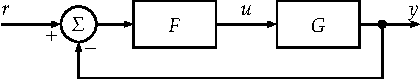
\includegraphics{feedback}
  \caption{\label{fig:feedback}%
    A simple illustration in a floating \envname{figure} environment.  Note that figure captions are always placed under the corresponding figure, and hence that the caption code should always appear at the end of the \envname{figure} environment.}
\end{figure}

\section{Hyperlinks}
%
For readers our the electronically published version of your thesis, as well as yourself while your are working on it, it is very convenient to have working hyperlinks in the document.

\subsection{Basic setup}
%
Basically, hyperlinks are obtained by using the \styname{hypreref} package. However, this package has quite a lot of compatibility issues with other packages, and knowledge about how to deal with these issues is coded into the \rtthesis class.  That is, all you should have to do to get hyperlinks in your document is to specify the \classoption{hyperref} option to \rtthesis.  The class options related to the linking infrastructure of the document are listed in \tableref{tab:hyperref}.

At the time of writing \rtthesis does not call \texcommand{hypersetup} with information about document title, keywords, and other information provided to \texcommand{setupThesis} (see \tableref{tab:setupThesis}).  If someone wants this, it shouldn't be hard to do.

\begin{table}[tbp]
  \centering
  \caption{\label{tab:hyperref}%
    Class options related to (hyper) linking infrastructure.}

  \begin{tabular}{l p{0.5\linewidth}}
    \toprule%
    \textbf{Class option} & \textbf{Meaning} \\
    \otoprule%
    \classoption{hyperref} & Turn on hyperlinks using the \styname{hyperref} package.  Default. \\
    \classoption{nohyperref} & Turn off hyperlinks, and compensate for commands no longer provided by the \styname{hyperref} package. \\
    \midrule%
    \classoption{backref} & Turn on bibliography back references.  Default. \\
    \classoption{nobackref} & Turn off bibliography back references.  (Currently required if you plan to use the features of \styname{bibunits}.)\\
    \bottomrule%
  \end{tabular}
\end{table}


\subsection{Hyperlinks and electronic publishing}
%
To make your dear hyperlinks survive all the way to the electronic publishing system, you may have to replace the file that is sent to e-press by LiU-tryck.  The problem is that LiU-tryck creates a compressed version of the file that is used in the printer, and the compression will remove nice features such as page numbers, hyperlinks, and bookmarks.  Fortunately, the guys at e-press seem to be understanding and will accept to publish a file that they receive directly from you.

\subsection{Page number formatting in the index}
%
If you use an index in your thesis, you will often want to change the formatting of certain page numbers in the index.  Without \styname{hyperref}, this could look like
{\verbatimsize
\begin{verbatim}
hyperlinks\index{hyperlinks|textit}
\end{verbatim}}
to get the page number for this occurrence of \emph{hyperlinks} to be typeset in italics.  The problem with this is that this page number will not be a hyperlink, while other page numbers will be hyperlinks to the correct page.  To get both italics and a hyperlink you need to define a special index formatting commands like the following.
{\verbatimsize
\begin{verbatim}
\newcommand{\hyperpageit}[1]{\textit{\hyperpage{#1}}}
\newcommand{\hyperpagebf}[1]{\textbf{\hyperpage{#1}}}
\newcommand{\hyperpagefootnote}[1]{\hyperpage{#1}n}
\end{verbatim}}

Now, you can write
{\verbatimsize
\begin{verbatim}
hyperlinks\index{hyperlinks|hyperpageit}
\end{verbatim}}
to get both italics and a hyperlink.  The \rtthesis class will provide a trivial definition of \texcommand{chapter} in case \styname{hyperref} is not loaded, so you may safely start to use the above definitions even if you are not sure whether you will use hyperlinks in the end.

\subsection{Friendlier hyperlinks}
%
The default mechanism for references in \LaTeX{}, being the command \texcommand{ref}, is modified as expected by the \styname{hyperref} package.  For instance, the number in “chapter~\ref{cha:rtthesis}” is linked to the beginning of the current chapter (if you click it, be sure to just the \emph{jump back} function of your \textsc{pdf} viewer to get back to here!).  However, all of “\hyperref[cha:rtthesis]{this}” is also a link to the same place.  That is, it is possible to other things than the number itself as links.  We could also make a reference that will never be linked, like in “chapter~\ref*{cha:rtthesis}”.

So, what's so friendly about this?  What I'm aiming at is that you can say “\hyperref[cha:rtthesis]{chapter~\ref*{cha:rtthesis}}”.  The code for this link is
{\verbatimsize
\begin{verbatim}
\hyperref[cha:rtthesis]{chapter~\ref*{cha:rtthesis}}
\end{verbatim}}

Of course, it is very annoying to repeat the key twice; first to point the hyperlink to the correct place, second to show the number of the chapter.  With the \texcommand{autoref} command from the \styname{hyperref} bundle, we get “\autoref{cha:rtthesis}”.  This is almost perfect.  The problem is that one cannot get an uppercase initial at the beginning of a sentence without redefining “chapter” to “Chapter“,
{\verbatimsize
\begin{verbatim}
\renewcommand{\Chaptername}{Chapter}
\end{verbatim}}
but then we will not get the nice lower case initial in the middle of a sentence.  Many authors don't bother about this and use uppercase initials irrespectively of where in a sentence the reference appears.

The only solution I (Henrik Tidefelt) knows of, is to define special commands for each type of reference.  A basic solution might look as follows.
{\verbatimsize
\begin{verbatim}
\newcommand{\chapterref}[1]{\hyperref[#1]{chapter~\ref*{#1}}}
\newcommand{\Chapterref}[1]{\hyperref[#1]{Chapter~\ref*{#1}}}
\end{verbatim}}

You should then use \texcommand{chapterref} in the middle of a sentence, and \texcommand{Chapterref} at the beginning of a sentence.  I you later decide that you want to have upper case initials everywhere, you just have to change your definitions to
{\verbatimsize
\begin{verbatim}
\newcommand{\chapterref}[1]{\hyperref[#1]{Chapter~\ref*{#1}}}
\newcommand{\Chapterref}[1]{\hyperref[#1]{Chapter~\ref*{#1}}}
\end{verbatim}}

A more complete solution will also provide commands for the plural forms “chapters” and “Chapters”.

It is also nice to use a similar technique for page references.  For instance, this chapter starts on \hyperref[cha:rtthesis]{page~\pageref*{cha:rtthesis}}, and such links can be created easily using a command like
{\verbatimsize
\begin{verbatim}
\newcommand{\pagepageref}[1]{\hyperref[#1]{page~\pageref*{#1}}}
\end{verbatim}}

Because of the many possible preferences for how to handle labels and references within documents, \rtthesis does not define any related commands.  The current section should give you some ideas of what can be achieved, and now it is up to you to design your own solution or borrow a solution from someone else (or simply stick with \texcommand{autoref} or the 1980's way of doing things)!

\section{Backreferences from the bibliography}
%
By default, \rtthesis uses the \styname{backref} package to put references from the bibliography back into the text.  The options for turning this feature on and off are listed in \tableref{tab:hyperref}.

By controlling this feature via the class, the choice whether to use it or not can be made orthogonal to the choice of whether to use \styname{hyperref} or not.

In addition to just loading \styname{backref}, \rtthesis will do a basic setup of the commands used to typeset the list of page numbers for each reference.  This behavior can easily be redefined without modifying the \rtthesis class file.  See the \styname{backref} documentation for details on how to do this!

\section{Using the \styname{bibentry} package}\label{sec:rtthesis:bibentry}
%
The \styname{bibentry} package makes it possible to use the information in the bibliography to present your publications at any place in the document.  In order to work independently of whether you use back references from the bibliography or not, you need to follow the pattern below each time you use the \texcommand{bibentry} command, where \texttt{KEY} is the same key to you publication that you would with use with any other citation command.

\begin{minipage}{1.0\linewidth}
  \verbatimsize
\begin{verbatim}
\begin{quotation}
  \nocite{KEY}\noindent
  \backrefparscanfalse\bibentry{KEY}.\backrefparscantrue
\end{quotation}
\end{verbatim}
\end{minipage}

To use the \envname{quotation} environment is just a suggestion — it will make the reference stand out by using a some what shorter text line width.  Note the period that follows the \texcommand{bibentry} command — the command leaves it up to you how to terminate the entry.  The \texcommand{nocite} command ensures that the reference appears in the bibliography, which is necessary to produce the entry.  The \texcommand{noindent} commands simply prevents the first line in the \envname{quotation} from being indented.  The commands \texcommand{backrefparscanfalse} and \texcommand{backrefparscantrue} are related to the \styname{backref} package used to produce back references from the bibliography, and should always surround the \texcommand{bibentry} command.  In case you have turned back references off using the \classoption{nobackref}, \rtthesis will provide substitutes for these two commands.


\section{Fonts}
%
Though basically not a task for a \LaTeX{} class, \rtthesis will assist in loading some font packages.  There are some class options that control this behavior, described below, and if these options are not good enough for you, you may have to make your own copy of the class and replace the font packages you don't like.  Options for font selection are listed in \tableref{tab:fonts}.

One reason, however, for letting \rtthesis handle the font selection is that this makes it possible for the class to do some things more intelligently.  At the moment, \rtthesis will help you make use of some of the goodies of KpFonts, if you choose to use that font.

\begin{table}[tbp]
  \centering
  \caption{\label{tab:fonts}%
    Class options related to fonts.  When slanted small caps are activated, theorem-like environments will use slanted text instead of italics.  The lower part of the table are examples of options that will be understood by the \styname{kpfonts} package, and are only meaningful in combination with the \classoption{kp} option.  (Note that options passed to \rtthesis, but that are not understood by \rtthesis will be passed on automatically by \LaTeX{} to loaded packages.)}

  \begin{tabular}{l p{0.5\linewidth}}
    \toprule%
    \textbf{Class option} & \textbf{Meaning} \\
    \otoprule%
    \classoption{kp} & Use KpFonts (Kepler) and activate slanted small caps.  Default.\\
    \classoption{times} & Use Times and deactivate slanted small caps.\\
    \classoption{lm} & Use Latin Modern and deactivate slanted small caps.\\
    \midrule%
    \classoption{largesmallcaps} & Let the small caps be slightly higher than an \emph{x}.  See the KpFonts documentation!\\
    \classoption{intlimits} & Placement of integration limits.  See the KpFonts documentation!\\
    \classoption{widermath} & Put just a little more horizontal space between entities in math mode.  See the KpFonts documentation!\\
    \bottomrule%
  \end{tabular}
\end{table}

\section{Hanging punctuation}
%
The \rtthesis class automatically loads the \styname{pdfcprot} package with its default settings.  It uses a pdf\TeX{} feature to make punctuation hang into the right margin.  If you don't like it, make your own copy of the class and comment out the line that loads the package.  One reason not to use it would be if your document will be (perhaps only occasionally) typeset using the old \TeX{} program, since this will lead to noticeable differences in the line breaks compared to when pdf\TeX{} is used.  No matter what you choose, make your choice \emph{before} you start working with the page breaks in your document!

\section{Paragraph breaks}
%
There are two common ways of visualizing paragraph breaks in a document, illustrated by the two examples below.  The look of paragraph breaks is controlled using the class options listed in \tableref{tab:parskip}.

\begin{table}[tbp]
  \centering
  \caption{\label{tab:parskip}%
    Class options related to formatting of paragraph breaks.}

  \begin{tabular}{l p{0.5\linewidth}}
    \toprule%
    \textbf{Class option} & \textbf{Meaning} \\
    \otoprule%
    \classoption{noparskip} & US style, see \exampleref{ex:paragraph-break-noparskip}.  Default.\\
    \classoption{parskip} & European style, see \exampleref{ex:paragraph-break-parskip}.\\
    \bottomrule%
  \end{tabular}
\end{table}

% \begin{example}[Default text]
%   This example does not mess with the lengths controlling the paragraph break format.  But you bet it ends in vmode!

% \end{example}

% It is good to see what it looks like if one puts text just below an example.

% \begin{example}[Default text]
%   This example does not mess with the lengths controlling the paragraph break format.  This one ends in hmode!
% \end{example}

\begin{example}[Indented first line]\label{ex:paragraph-break-noparskip}%
  \setlength{\parskip}{0pt}%
  \setlength{\parindent}{1.5em}%
  This style is still the most common.  It is particularly dominant in text written in the US.

  It is a matter of style whether to omit the indentation of the first line after a sectioning command such as \texcommand{chapter} or \texcommand{subsection}.  The omission is typically automated, but can also be enforced using the  \texcommand{noindent} command.

  One drawback of not having vertical space between paragraphs is that it will be harder for pdf\TeX{} to find good places for page breaks, compared to the option shown below.  If you like compact documents, however, this is the option for you!

  For testing purposes, this example ends with a paragraph break, so that \TeX{} is in \emph{vmode} at the end.  You should always avoid this, but the class will try to compensate for your mistakes\ldots

\end{example}

\begin{example}[Vertical white space]\label{ex:paragraph-break-parskip}%
  \setlength{\parskip}{1ex}%
  \setlength{\parindent}{0pt}%
  This style is still increasing in popularity.  It is rather common in modern texts written in Europe, and the style has received special attention from the Netherlands \TeX{} user group \emph{Nederlandstalige \TeX{} Gebruikersgroep, \textsc{ntg}}.  Their efforts can be used through their variants of the standard \LaTeX{} classes.

  Unfortunately, the \textsc{ntg} classes are not compatible with \rtthesis, and the solution provided by the \styname{parskip} package is only part of the solution.  Hence, \rtthesis will do more than just loading the \styname{parskip} package for you if you specify the \classoption{parskip} option.

  A good reason to put code related paragraph breaks in the class file is that all the small adjustments that different people come up with can be put in one placed so that they are accessible to future users of the class.
\end{example}

\section{Page breaks}\label{sec:tipt:page-breaking}
%
There is a whole lot to say about how to obtain nice page breaks.  You will find some recommendations below, but do not use this document as your ultimate reference on this topic!  (This document itself contains some really nasty page breaks --- at least at the time of writing this --- as a result of not paying any attention at all to the problem.  It would simply bee too time-consuming to keep adjusting the page breaks each time the document is edited.)
\begin{itemize}
\item
  Take no consideration of page breaks until page breaking is the only aspect of your thesis that remains to be taken care of!  Page breaking involves a lot of manual intervention of the automatic mechanisms in pdf\TeX{}, and as soon as you have started to intervene, any further changes to the text will risk to ruin your page breaking fixes, and may even lead to worse results than before since the automatic page breaking has been tampered with.
\item
  First thing to try is to make changes to the text to help the automatic page breaking mechanism.  Try to make sentences longer or shorter depending on the situation.  Since this will not tamper with the automatic page breaking mechanism, this option will incur the least loss of maintainability of your document.
\item
  Can the location of floats be changed to improve page breaks?  Play around with exactly where in your source files the code for the floating environments appears!
\item
  You may also try to force early page breaks using the \texcommand{Needspace*} command.  For instance, putting
{\verbatimsize
\begin{verbatim}
\Needspace*{2\baselineskip}
\end{verbatim}}
before a paragraph will cause a page break if there is not enough vertical space on the page to hold two lines of text.  The good thing about this option is that your intervention will cause no harm if the \texcommand{Needspace*} command appears in the middle of a page.  The bad thing about this option is that it may cause remaining vertical space on the broken page to be stretched quite badly.  You should always check that the resulting page looks OK!

For more information, and related commands, see the documentation for the \styname{needspace} package!
\item
  The last option is to play with the vertical size of individual pages.  For instance, putting
{\verbatimsize
\begin{verbatim}
\enlargethispage{2\baselineskip}
\end{verbatim}}
before a paragraph you would like to fit into the current page will make space for two extra lines of text.  This avoids the bad stretching of vertical space that the \texcommand{Needspace*} option may cause.  However, if you would make other changes that makes tampering with the page size unnecessary, it will be very time-consuming to detect this and remove the no longer needed \texcommand{enlargethispage} command.
\end{itemize}

Note that manual page breaking is a time-consuming task.  Make sure to have at least one full day allocated to page breaking before you submit your thesis for print!

\section{Input encoding}
%
Two input encodings are supported, being \mbox{latin-1} and \mbox{\textsc{utf}-8}.  The choice of input encoding should be made via the \rtthesis class, so that the class can use the correct encoding to define certain global strings.  The input encoding options are listed in \tableref{tab:inputenc}.

\begin{table}[tbp]
  \centering
  \caption{\label{tab:inputenc}%
    Class options related to input encodings.  Note that there is no default; \rtthesis requires one of these options to be passed explicitly.}

  \begin{tabular}{l p{0.5\linewidth}}
    \toprule%
    \textbf{Class option} & \textbf{Meaning} \\
    \otoprule%
    \classoption{latin1} & Simply use \styname{inputenc} with option \classoption{latin1}. \\
    \classoption{utf8} & Use \styname{inputenc} with option \classoption{utf8}, and define some additional characters. \\
    \bottomrule%
  \end{tabular}
\end{table}

Choose \mbox{latin-1} if you depend on lots of files using this encoding, and do not want to change the encoding of these files.  Changing the encoding of a file is easy both in Emacs and using the \emph{iconv} command line utility.  The \mbox{latin-1} encoding is the default in \rtthesis, but the choice can be made explicit by passing the \classoption{latin1} option to the class.

Choose \mbox{\textsc{utf}-8} to be able to type many more characters directly in your \LaTeX{} sources compared to \mbox{latin-1}.  For instance, names of foreign authors often use characters that cannot be entered directly using \mbox{latin-1}.  In \mbox{\textsc{utf}-8}, most of these as well as special punctuation characters such as double quotes and various dashes can be entered directly in the source.  Use the \classoption{utf8} class option if your files are encoded in \mbox{\textsc{utf}-8}.

The current implementation of \mbox{\textsc{utf}-8} in the \styname{inputenc} package only defines the input encoding for characters that have corresponding glyphs in active fonts (see the \styname{inputenc} documentation for details).  This means that some characters that \TeX{} would build by combining several glyphs will not be defined by \styname{inputenc}.  If the \classoption{utf8} is given, \rtthesis will define a list of additional characters by inclusion of the package \styname{rtthesis-utf8-ext}.  If you need additional characters, you should make your own package similar to \styname{rtthesis-utf8-ext}, and then let the maintainer of \rtthesis know, so that the additional characters may be added to \styname{rtthesis-utf8-ext} so that others can use them in the future.  Note that \styname{rtthesis-utf8-ext} may be a useful package also when you are not using the \rtthesis class.

It is easy to set up Emacs so that it uses the \mbox{\textsc{utf}-8} encoding for your \TeX{} files, but it is out of the scope of the current document to give further explanations here.


\section{\rtthesis and \styname{natbib}}
%
Interoperability with different bibliography packages is a tricky issue.  It has been a design decision to try to support at least \styname{natbib}, at the cost of loosing compatibility with other packages such as \styname{jurabib}.  The core of the problem is package loading order, requiring \styname{natbib} to be loaded very early on in the class.  To pass options to \styname{natbib}, pass them as global class options to \rtthesis.  Note that the default options for \styname{natbib} are quite reasonable, and see \tableref{tab:natbib} for examples of other options that \styname{natbib} will pick up.  If you know how to resolve the conflict with the \styname{natbib} option \classoption{usebibunits}, let the \rtthesis maintainer know!

\begin{table}[tbp]
  \centering
  \caption{\label{tab:natbib}%
    Class options related to the \styname{natbib} package.  Note that options can be passed to \styname{natbib} by passing them as global class options to \rtthesis.  See the \styname{natbib} documentation for more useful options.}

  \begin{tabular}{l p{0.5\linewidth}}
    \toprule%
    \textbf{Class option} & \textbf{Meaning} \\
    \otoprule%
    \classoption{authoryear} & Default option of \styname{natbib} --- no need to specify.\\
    \classoption{round} & Default option of \styname{natbib} --- no need to specify.\\
    \classoption{colon} & Default option of \styname{natbib} --- no need to specify.\\
    \midrule%
    \classoption{square} & Example of option that \styname{natbib} will pick up (alternative to \classoption{round}).\\
    \classoption{comma} & Example of option that \styname{natbib} will pick up (alternative to \classoption{colon}).\\
    \midrule%
    \classoption{numbers} & Conflicting \styname{natbib} option --- forbidden in combination with \classoption{usebibunits}, see \classoption{forcenumbers} below.\\
    \classoption{forcenumbers} & Enforce option \classoption{numbers} to be passed to \styname{natbib} (alternative to \classoption{authoryear}) --- it's up to you to resolve the conflict.\\
    \bottomrule%
  \end{tabular}
\end{table}


\section{The lists of previous theses}
%
The lists of previous licentiate's and PhD theses can be found in \textfilename{liclist.tex} and \textfilename{phdlist.tex}, respectively, and the appropriate one of the is automatically included at the end of your thesis.  Both files are found in the directory\\
\textfilename{\$TEXMFGROUPLOCAL/tex/latex/rt/rtthesis} .

Note that it is \emph{your responsibility} to make sure that your thesis is added to the appropriate list after you have sent it to print but before the next thesis of the same kind is printed.  If other people are writing theses at the same time as you, you will have to coordinate your moves in order to make sure that the lists get updated in the correct order.  To get your thesis added to the appropriate list, you simply send an email with information about your thesis to the \rtthesis maintainer.  The information shall be in one of the following formats:

{\verbatimsize
\begin{verbatim}
\licitem{J.~Doe}{Title}{Thesis No}{YYYY}
\end{verbatim}}

or

{\verbatimsize
\begin{verbatim}
\phditem{J.~Doe}{Title}{Theis No}{YYYY}{ISBN}
\end{verbatim}}

It is a good idea to make a copy of the file you need when it is time to print.  If you don't make a copy, and then compile your thesis again at a later time, the list will be wrong because it will include at least one thesis that wasn't prior to yours — namely your own!


\section{Compilation theses}
%
The \rtthesis class aims to support the production of both monographs and compilation theses.  There is a compilation thesis example included with \rtthesis.  Please have a look at that while reading the sections below!


\subsection{Including publications in your thesis}
%
It is assumed that included publications shall be compiled together with the rest of your thesis, as opposed to being included as exactly the way the look where published.  Under this assumption, it is reasonable to expect things such as a suitable chapter numbering, and that the global table of contents includes the sections withing publications.  Note that it would be rather difficult to get things such as the table of contents and other infrastructure right if publications were to be included by direct \textsc{pdf} inclusion.

The \envname{papers} environment provided by \rtthesis will redefine commands and set up some additional commands to support the inclusion of \LaTeX{} sources of your publication.  It is recommended that the environment is placed in a second part of the thesis.  Inside the environment, the \texcommand{chapter} command is redefined to both start a new chapter and set up the title of the publication to be included in the same chapter.  Chapters will be labeled with letters instead of numbers, so it is up to you to make a clear distinction between referencing an appendix chapter and a publication chapter.

If the title of a publication is too long to fit in the page header, you may follow the \texcommand{chaptermark} command by a \texcommand{chaptermark} command.  Since the \texcommand{chaptermark} command takes an optional argument to be used in the table of contents, there are three different variations of the publication title that can be defined.

The word for publications used by \rtthesis is \emph{paper}; it will appear both on the chapter title page and in page headers.  To change this to something else, you simply have to redefine \texcommand{chaptername} to something else inside the \envname{papers} environment.

After setting up the publication title, the \texcommand{author} command should be used to set up the list of authors.  It works as usual, but sports two special \rtthesis commands that should be used when there are two author affiliations;  put \texcommand{authorleft} immediately after author names who's affiliation should appear to the left below the list of authors, and put \texcommand{authorright} after the other authors.  There is currently no support for more than two different affiliations.

In case there is only one affiliation, that affiliation is given by \texcommand{paperaffiliation} (which should be set once and for all to your own affiliation), and you use the \texcommand{email} command to specify the list of email addresses to the authors.

In case of two affiliations, you call the commands \texcommand{affilblockleft} ,\texcommand{affilblockright}, \texcommand{emailleft}, and \texcommand{emailright} with the appropriate arguments.  Note that one of the two affiliation block arguments should simply be \texcommand{paperaffiliation}.

Additional information about the publication is given in after \texcommand{item} commands inside the \envname{paperinfo} environment.  In addition to the items given, the environment automatically starts with one item displaying the author information (without any marks related to affiliation blocks).  Three commands are defined by \rtthesis to simplify consistent formatting of additional information.
\begin{itemize}
\item \texcommand{paperedited{\emph{bib-key}}} — For ordinary publications.  The extent to which the publication has been edited should be state clearly.  The bibliography entry will be formatted using the technique described in \sectionref{sec:rtthesis:bibentry}.
\item \texcommand{paperprelver{\emph{ISY-report-number}}} — For publications for which there is only a preliminary version available.  The preliminary version should be published as a technical report at the department, and as no bibliography keys are involved, the technical report will not be listed in any the bibliography.
\item \texcommand{papertechrep{\emph{ISY-report-number}}} — For publications that are not yet even preliminary versions of something.  These too should be published as technical reports at the department, and will not appear in the bibliography.
\end{itemize}

At this point the chapter title page will be finished.   The next step is to make a nice title and abstract for your publication on the following odd page.  Use \texcommand{maketitle} or \texcommand{maketitletwoaffil} depending on whether you set up one or two affiliation blocks.  Then put the publication abstract inside the \envname{abstract} environment.

After this point, you should just be able to include the source of your publication, with \texcommand{section} as the topmost sectioning command (since the publication itself is a chapter of your thesis).

Finally, you must decide where your references should go.  Should there be one global bibliography for the whole thesis, or should there be one bibliography for each publication.  This is the topic of the next section.

\subsection{Compilation theses and bibliographies}
%
If you are fine with having just one global bibliography for the whole thesis, everything should work out of the box.  Hence, this section will try to describe how to do in order to get one bibliography for the background part of your thesis, and one for each publication.

The \rtthesis class only supports this by relying on the \styname{bibunits} package.  Due to package loading order issues, it should always be loaded by passing \classoption{usebibunits} to \rtthesis.  Note that some of the \styname{bibunits} commands appears to be incompatible with bibliography back references, so you need to pass the \classoption{nobackref} to \rtthesis if you plan to use the \styname{bibunits} features.

\begin{remark}
  There is a very interesting package called \styname{biblatex} which is currently in beta version.  Hopefully, it will let us drop the messy packages \styname{bibunits} and \styname{backref}.  You are invited to try this package, and if you find it to work satisfactory it should probably be incorporated in \rtthesis.  Future maintainers of \rtthesis are strongly encouraged to find out what \styname{biblatex} can do for us!
\end{remark}

Use the command \texcommand{defaultbibliography} to specify the bibliography files to use for all of the per-publication bibliographies, and use \texcommand{defaultbibliographystyle} to select the bibliography style, see the \styname{bibunits} documentation for details.

To get an individual bibliography for a publication, you should just have to include that chapter in a \envname{bibunit} environment, and call \texcommand{putbib} where you want the bibliography to appear.  Here, the \texcommand{putbib} command will be redefined by \rtthesis in order to make the bibliography appear in the table of contents.

A bibliography for references that appear in the background part of your thesis are produced as usual with the \texcommand{bibliography} command.  (It might be good to know that \rtthesis will automatically issue the \texcommand{nobibliography*} command in order to make the \styname{bibentry} package work as you would expect.)

\section{Master's theses}\label{sec:msc}
%
The \styname{liuthesis} class by Gustaf Hendeby was developed for the production of master's theses at Linköping University.  The class knows how to create the special pages required by several departments, and in the summer of 2011 this capability was merged into \rtthesis.  This makes it convenient to produce a master's thesis at Linköping University using \rtthesis instead of \styname{liuthesis}, allowing a wider audience to benefit from the more active development of \rtthesis.\footnote{The \LaTeX{} class files tend to be maintained by PhD students, and PhD students have a tendency to be more interested in maintaining the class files for writing licentiate's and PhD theses than class files for master's theses.}

This section describes how to use \rtthesis to produce a master's thesis.  To begin, pass \emph{msc} as the value for the key \emph{type} in the call to \texcommand{setupThesis}, and select your department using the key \emph{department}.  More details are given below, and the reader is encouraged to study the bundled example in order to get a better overall picture.

\subsection{Master's thesis setup}
%
In addition to the pieces of information given to \texcommand{setupThesis} for licentiate's and PhD theses (see \tableref{tab:setupThesis}), there are some that only apply to master's theses.  These are listed in \tableref{tab:setupThesis-msc}.

\begin{table}[tbp]
  \centering
  \caption{\label{tab:setupThesis-msc}%
    \texcommand{setupThesis} key-value pairs for master's theses, in addition to those listed in \tableref{tab:setupThesis}.  Note that values that include white space are surrounded by braces.}

  \begin{tabular}{>{\ttfamily}r !{\texttt{=}} >{\ttfamily}l l}
    \toprule%
    \textbf{Key} & \textbf{Example value} & \textbf{Comment} \\
    \otoprule%
    swetitle & \{Svensk titel\} & Title in Swedish\\
    swesubtitle & \{Bra grejer\} & Optional Swedish subtitle\\
    month & 4 & \\
    day & 9 & \\
    subject & reglerteknik & \\
    site & \{Bosses AB i Linkan\} & \\
    division & \{Avdelningenrt\ldots\} & \\
    department & isy & See \tableref{tab:department} \\
    examiner & \{Lena Lärare\ldots\} & Details given below \\
    supervisor & \{Doktorand Si\} & Details given below \\
    keywords & \{this, that\} & Appears on library page \\
    isrn & LiTH-ISY-EX\ldots & See below \\
    url & \{http://\ldots\} & Thesis download \textsc{url}, see below \\
    \bottomrule%
  \end{tabular}
\end{table}

The value for the key \emph{department} must be one of the special values listed in \tableref{tab:department}.  This setting controls both the department name and address, as well as how the special pages of the thesis are formatted.  Please help the \rtthesis maintainer to keep the special pages for your department up to date.

In the values for the keys \emph{examiner} and \emph{supervisor}, multiple persons should be separated using \texcommand{AND}, and the affiliation of a person should appear after \texcommand{AT}, like this:
{\verbatimsize
\begin{verbatim}
  supervisor={Doktorand Si \AT \textsc{isy}, Linköpings universitet
         \AND Ingenjör Så \AT Företaget},
\end{verbatim}}

The \textsc{isrn}\footnote{The \textsc{iso} standard for \textsc{isrn} was withdrawn in 2007, but the report numbering system is still in use at Linköping University.} should be something like
{\verbatimsize
\begin{verbatim}
  isrn=LITH-ISY-EX-{}-YY/NNNN-{}-SE
\end{verbatim}}
but the format varies between different departments.  Note that if the report identifier contains two or three consecutive dashes, they have to be separated by empty braces in the input to prevent \LaTeX{} from interpreting them as one character.  The thesis download \textsc{url} should be something like
{\verbatimsize
\begin{verbatim}
  url={http://urn.kb.se/resolve?urn=urn:nbn:se:liu:diva-XXXXX}
\end{verbatim}}
The exact details regarding the report number and \textsc{url} will be given to you by the librarian when you register your thesis.

\begin{table}[tbp]
  \centering
  \caption{\label{tab:department}%
    Recognized values for the key \emph{department} in \tableref{tab:setupThesis-msc}.}

  \begin{tabular}{>{\ttfamily}c p{0.45\linewidth} l}
    \toprule%
    \textbf{department} & \textbf{Department of\ldots} & \textbf{Updated}\\
    \otoprule%
    ida & Computer and Information Science & Not after 2008-08-01\\
    ifm & Physics, Chemistry and Biology & 2011-07-03\\
    iei & Management and Engineering & \emph{Out of date!}\\
    isy & Electrical Engineering & 2011-07-03\\
    itn & Science and Technology & 2011-07-03\\
    mai & Mathematics & 2011-07-03\\
    \bottomrule%
  \end{tabular}
\end{table}

\subsection{Special pages}
%
The requirements on a master's thesis include that certain information go on the front page and title page of the thesis.  Further, a library page for cataloging purposes is required at the beginning of the thesis, and a page with copyright information is required at the end.  The copyright page is automatically added at the end.  The other special pages can be produced using the macros \texcommand{makeFrontPage}, \texcommand{maketitle} (as usual), and \texcommand{makeLibraryPage}.  These macros are meant to be invoked more or less immediately after \texcommand{begin\{document\}}, see the bundled example for details.  Note that in the printed report, the front page should be replaced by the cover, and the library page is \emph{probably} meant to be on a loose piece of paper inserted between the cover and the title page.

There is no magic that puts the correct abstract on the library page, but the abstract must be given as an argument to \texcommand{makeLibraryPage}.  To make sure that this is exactly the same as the abstract in the thesis, it is recommended that you write the abstract text without any surrounding \envname{abstract} environment in a separate file, say \textfilename{svensk-sammanfattning.tex}.  Then you can use this file twice, like this:
{\verbatimsize
\begin{verbatim}
\makeLibraryPage{Det här som vi har hållit på med är jätteviktigt faktiskt och det vi gjort blev bara sååå bra.  Kanske inte helt otippat, men det glass är sååå gott!

Förresten har vi blivit bäst på att skriva rapporter, så nu ska ska vi inte gå in närmare på några detaljer såhär i sammanfattningen.
}

\begin{abstract}[swedish]
  Det här som vi har hållit på med är jätteviktigt faktiskt och det vi gjort blev bara sååå bra.  Kanske inte helt otippat, men det glass är sååå gott!

Förresten har vi blivit bäst på att skriva rapporter, så nu ska ska vi inte gå in närmare på några detaljer såhär i sammanfattningen.

\end{abstract}
\end{verbatim}}
(The bundled example uses this technique.)

\subsection{Choice of language}
%
If your main report language will be Swedish, put
{\verbatimsize
\begin{verbatim}
\selectlanguage{swedish}
\end{verbatim}}
right after
{\verbatimsize
\begin{verbatim}
\begin{document}
\end{verbatim}}
Also make sure to provide the thesis title (and possibly subtitle) in Swedish via the keys \emph{swetitle} and \emph{swesubtitle} to \texcommand{setupThesis}.  You may then omit writing an abstract in English.

If your main report language will be English you don't need to change the default choice of language.  However, you must provide a thesis title both in English and Swedish, and the thesis should contain abstracts in both English and Swedish.


\section{Compiling the document}
%
Using all the current features of \rtthesis, the following sequence of steps is usually sufficient to compile your document.  Let us assume your main file is named \textfilename{main.tex}.
\begin{itemize}
\item
  First run
{\verbatimsize
\begin{verbatim}
pdflatex main
\end{verbatim}}
  to scan your document for references, labels, and index items.
\item
  Then run
{\verbatimsize
\begin{verbatim}
bibtex main
\end{verbatim}}
  to extract relevant references from your bibliography file(s).  If you are using the \styname{bibunits} package, you also have to process some additional files;
{\verbatimsize
\begin{verbatim}
bibtex bu1; bibtex bu2; ...; bibtex bun
\end{verbatim}}
\item
  If you have an index in your document, run
{\verbatimsize
\begin{verbatim}
makeindex main
\end{verbatim}}
  to format it.
\item
  Then run
{\verbatimsize
\begin{verbatim}
pdflatex main
\end{verbatim}}
  to insert references in the typeset document.  This will typically move things around, and your page references will be invalidated.
\item
  Hopefully, it is enough to run
{\verbatimsize
\begin{verbatim}
pdflatex main
\end{verbatim}}
  once more now to get the page references right.  You will get a warning if you need to repeat this step.
\end{itemize}

In addition to the steps above, certain auxiliary files must be deleted when certain features of the class are turned on or off.  In particular, turning hyperlinks on or off requires the following.
{\verbatimsize
\begin{verbatim}
rm main.aux main.toc main.ind
\end{verbatim}}

\section{Generating a thesis cover and the “spikblad”}
%
A thesis cover can be created by making a file that contains the \texcommand{makecover} command.  For example, given that \textfilename{mythesis.sty} invokes the \texcommand{setupThesis} command with the necessary information (see \tableref{tab:setupThesis}), a PhD thesis cover can be made as follows.

\begin{minipage}{1.0\linewidth}
  \verbatimsize
\begin{verbatim}
\documentclass[utf8,phd]{rtthesis}
\usepackage{mythesis}

\makecover
\end{verbatim}
\end{minipage}

Note that while all licentiate's theses should have the same cover, there is no standard (but many rules set by the university!) for the PhD theses.  The \texcommand{makecover} command gives a “classic” cover that quite a few people have used over the years.  This cover might also be useful as a means to compile the information needed when LiU-Tryck (or some other printing company) designs a more artistic cover.

For a dissertation, there should always be a “spikblad” (literally, \emph{nailing sheet}).  Such an information sheet can be generated easily if the English abstract is put in a separate file.  In this case, the same abstract can be included both in the thesis and in a separate file that defines the “spikblad”.  For a licentiate's thesis presentation, a similar information sheet should be produced.  The monograph example demonstrates how to created these, see the files \textfilename{spikblad.tex} (for dissertations) and \textfilename{licinfo.tex} (for licentiate's thesis presentations).


\section{Required logotypes (not included with \rtthesis)}
%
\Tableref{tab:logos} lists files with logotype graphics that are needed by \rtthesis.  They are not part of the \rtthesis bundle since they are used in many other contexts as well.  Users at the Division of Automatic Control should have access to these files via the group's common texmf tree, but in order to be able to work at home you will have to make sure one way or another that the files are installed.

Beware that the university changes logos quite often. Make sure that there are no new versions of the logos you use.  If the logos are old, please, let the \rtthesis maintainer know so that the files get updated at the central location.

\begin{table}[tbp]
  \centering
  \caption{\label{tab:logos}%
    Files with logotype graphics used by \rtthesis.  Use the command \texttt{kpsewhich} to find where the files are located!}

  \begin{tabular}{l p{0.5\linewidth}}
    \toprule%
    \textbf{Filename} & \textbf{Use} \\
    \otoprule%
    \textfilename{LinkUniv\usc{}sigill\usc{}sv.pdf} & For the cover and the first page in PhD theses.\\
    \textfilename{LiTH\usc{}staende\usc{}eng\usc{}sv.pdf} & For the cover of both licentiate's and PhD theses.\\
    \textfilename{rtlogo\usc{}tall.pdf} & For the first page in licentiate's theses.\\
    \bottomrule%
  \end{tabular}
\end{table}

\section{Compatibility with standard packages}
%
Incompatibilities between different packages is a problem that quickly becomes quite an issue when the list of packages used in a document grows beyond just a few.  It may sound strange, but it is because of compatibility problems that \rtthesis includes a rather long list of packages for you.  The reason is that this allows knowledge about package loading order requirements and various workarounds, to be encoded in the class file.

No list of packages included by \rtthesis will be presented here, but you should check the class file directly to be sure that you always get the correct answer to whether a package is included or not (or you can just read the compilation output).

Packages with no known compatibility issues will generally not be included by \rtthesis unless needed by the class itself.  The following list contains some examples of useful packages that are not included by \rtthesis.  They \emph{should} be compatible with \rtthesis.  Please let the \rtthesis maintainer know if any of these are no longer compatible, or if you have suggestions for other packages that should be mentioned here.
\begin{itemize}
  \item \styname{nextpage} — page break control
  \item \styname{algorithm} — code listings
  \item \styname{listings} — code listings
  \item \styname{SIunits} — physical dimensions
  \item \styname{pmat} — partitioned matrices
  \item \styname{bm} — bold math
  \item \styname{footmisc} — extras for footnotes
  \item \styname{dcolumn} — decimal point alignment in tables (the already included \styname{array} can also do this)
  \item \styname{lettrine} — start chapter with fancy letter
  \item \styname{supertabular} — multi-page tables
  \item \styname{longtable} — multi-page tables
  \item \styname{multirow} — tabular entries occupying more than one row
\end{itemize}

\clearemptydoublepage
\backmatter

\bibliography{IEEEfull,myrefs}

\printindex

\end{document}
